\documentclass[twoside]{book}

% Packages required by doxygen
\usepackage{fixltx2e}
\usepackage{calc}
\usepackage{doxygen}
\usepackage[export]{adjustbox} % also loads graphicx
\usepackage{graphicx}
\usepackage[utf8]{inputenc}
\usepackage{makeidx}
\usepackage{multicol}
\usepackage{multirow}
\PassOptionsToPackage{warn}{textcomp}
\usepackage{textcomp}
\usepackage[nointegrals]{wasysym}
\usepackage[table]{xcolor}

% Font selection
\usepackage[T1]{fontenc}
\usepackage[scaled=.90]{helvet}
\usepackage{courier}
\usepackage{amssymb}
\usepackage{sectsty}
\renewcommand{\familydefault}{\sfdefault}
\allsectionsfont{%
  \fontseries{bc}\selectfont%
  \color{darkgray}%
}
\renewcommand{\DoxyLabelFont}{%
  \fontseries{bc}\selectfont%
  \color{darkgray}%
}
\newcommand{\+}{\discretionary{\mbox{\scriptsize$\hookleftarrow$}}{}{}}

% Page & text layout
\usepackage{geometry}
\geometry{%
  a4paper,%
  top=2.5cm,%
  bottom=2.5cm,%
  left=2.5cm,%
  right=2.5cm%
}
\tolerance=750
\hfuzz=15pt
\hbadness=750
\setlength{\emergencystretch}{15pt}
\setlength{\parindent}{0cm}
\setlength{\parskip}{3ex plus 2ex minus 2ex}
\makeatletter
\renewcommand{\paragraph}{%
  \@startsection{paragraph}{4}{0ex}{-1.0ex}{1.0ex}{%
    \normalfont\normalsize\bfseries\SS@parafont%
  }%
}
\renewcommand{\subparagraph}{%
  \@startsection{subparagraph}{5}{0ex}{-1.0ex}{1.0ex}{%
    \normalfont\normalsize\bfseries\SS@subparafont%
  }%
}
\makeatother

% Headers & footers
\usepackage{fancyhdr}
\pagestyle{fancyplain}
\fancyhead[LE]{\fancyplain{}{\bfseries\thepage}}
\fancyhead[CE]{\fancyplain{}{}}
\fancyhead[RE]{\fancyplain{}{\bfseries\leftmark}}
\fancyhead[LO]{\fancyplain{}{\bfseries\rightmark}}
\fancyhead[CO]{\fancyplain{}{}}
\fancyhead[RO]{\fancyplain{}{\bfseries\thepage}}
\fancyfoot[LE]{\fancyplain{}{}}
\fancyfoot[CE]{\fancyplain{}{}}
\fancyfoot[RE]{\fancyplain{}{\bfseries\scriptsize Generated by Doxygen }}
\fancyfoot[LO]{\fancyplain{}{\bfseries\scriptsize Generated by Doxygen }}
\fancyfoot[CO]{\fancyplain{}{}}
\fancyfoot[RO]{\fancyplain{}{}}
\renewcommand{\footrulewidth}{0.4pt}
\renewcommand{\chaptermark}[1]{%
  \markboth{#1}{}%
}
\renewcommand{\sectionmark}[1]{%
  \markright{\thesection\ #1}%
}

% Indices & bibliography
\usepackage{natbib}
\usepackage[titles]{tocloft}
\setcounter{tocdepth}{3}
\setcounter{secnumdepth}{5}
\makeindex

% Hyperlinks (required, but should be loaded last)
\usepackage{ifpdf}
\ifpdf
  \usepackage[pdftex,pagebackref=true]{hyperref}
\else
  \usepackage[ps2pdf,pagebackref=true]{hyperref}
\fi
\hypersetup{%
  colorlinks=true,%
  linkcolor=blue,%
  citecolor=blue,%
  unicode%
}

% Custom commands
\newcommand{\clearemptydoublepage}{%
  \newpage{\pagestyle{empty}\cleardoublepage}%
}

\usepackage{caption}
\captionsetup{labelsep=space,justification=centering,font={bf},singlelinecheck=off,skip=4pt,position=top}

%===== C O N T E N T S =====

\begin{document}

% Titlepage & ToC
\hypersetup{pageanchor=false,
             bookmarksnumbered=true,
             pdfencoding=unicode
            }
\pagenumbering{roman}
\begin{titlepage}
\vspace*{7cm}
\begin{center}%
{\Large G\+NU P\+R\+O\+L\+OG with U\+T\+F8 support }\\
\vspace*{1cm}
{\large Generated by Doxygen 1.8.11}\\
\end{center}
\end{titlepage}
\clearemptydoublepage
\tableofcontents
\clearemptydoublepage
\pagenumbering{arabic}
\hypersetup{pageanchor=true}

%--- Begin generated contents ---
\chapter{Data Structure Index}
\section{Data Structures}
Here are the data structures with brief descriptions\+:\begin{DoxyCompactList}
\item\contentsline{section}{\hyperlink{struct__excp__lst}{\+\_\+excp\+\_\+lst} }{\pageref{struct__excp__lst}}{}
\item\contentsline{section}{\hyperlink{structAliasInf}{Alias\+Inf} }{\pageref{structAliasInf}}{}
\item\contentsline{section}{\hyperlink{structArgInf}{Arg\+Inf} }{\pageref{structArgInf}}{}
\item\contentsline{section}{\hyperlink{structArithInf}{Arith\+Inf} }{\pageref{structArithInf}}{}
\item\contentsline{section}{\hyperlink{structAsmLine}{Asm\+Line} }{\pageref{structAsmLine}}{}
\item\contentsline{section}{\hyperlink{structAtomInf}{Atom\+Inf} }{\pageref{structAtomInf}}{}
\item\contentsline{section}{\hyperlink{structAtomProp}{Atom\+Prop} }{\pageref{structAtomProp}}{}
\item\contentsline{section}{\hyperlink{unionBCWord}{B\+C\+Word} }{\pageref{unionBCWord}}{}
\item\contentsline{section}{\hyperlink{structbtnode}{btnode} }{\pageref{structbtnode}}{}
\item\contentsline{section}{\hyperlink{structBTString}{B\+T\+String} }{\pageref{structBTString}}{}
\item\contentsline{section}{\hyperlink{unionC64To32}{C64\+To32} }{\pageref{unionC64To32}}{}
\item\contentsline{section}{\hyperlink{structCmdInf}{Cmd\+Inf} }{\pageref{structCmdInf}}{}
\item\contentsline{section}{\hyperlink{structCodeInf}{Code\+Inf} }{\pageref{structCodeInf}}{}
\item\contentsline{section}{\hyperlink{structcomp__node}{comp\+\_\+node} }{\pageref{structcomp__node}}{}
\item\contentsline{section}{\hyperlink{structcptcell}{cptcell} }{\pageref{structcptcell}}{}
\item\contentsline{section}{\hyperlink{structCPTMatch}{C\+P\+T\+Match} }{\pageref{structCPTMatch}}{}
\item\contentsline{section}{\hyperlink{structcptnode}{cptnode} }{\pageref{structcptnode}}{}
\item\contentsline{section}{\hyperlink{structCPTStat}{C\+P\+T\+Stat} }{\pageref{structCPTStat}}{}
\item\contentsline{section}{\hyperlink{structD2ChCell}{D2\+Ch\+Cell} }{\pageref{structD2ChCell}}{}
\item\contentsline{section}{\hyperlink{structD2ChHdr}{D2\+Ch\+Hdr} }{\pageref{structD2ChHdr}}{}
\item\contentsline{section}{\hyperlink{unionDblInt}{Dbl\+Int} }{\pageref{unionDblInt}}{}
\item\contentsline{section}{\hyperlink{structdirectinf}{directinf} }{\pageref{structdirectinf}}{}
\item\contentsline{section}{\hyperlink{structDSwtInf}{D\+Swt\+Inf} }{\pageref{structDSwtInf}}{}
\item\contentsline{section}{\hyperlink{structdyncinf}{dyncinf} }{\pageref{structdyncinf}}{}
\item\contentsline{section}{\hyperlink{structdynpinf}{dynpinf} }{\pageref{structdynpinf}}{}
\item\contentsline{section}{\hyperlink{structDynScan}{Dyn\+Scan} }{\pageref{structDynScan}}{}
\item\contentsline{section}{\hyperlink{structFileInf}{File\+Inf} }{\pageref{structFileInf}}{}
\item\contentsline{section}{\hyperlink{structflag__inf}{flag\+\_\+inf} }{\pageref{structflag__inf}}{}
\item\contentsline{section}{\hyperlink{structGTarget}{G\+Target} }{\pageref{structGTarget}}{}
\item\contentsline{section}{\hyperlink{structgundo}{gundo} }{\pageref{structgundo}}{}
\item\contentsline{section}{\hyperlink{structGVarElt}{G\+Var\+Elt} }{\pageref{structGVarElt}}{}
\item\contentsline{section}{\hyperlink{structhash__node}{hash\+\_\+node} }{\pageref{structhash__node}}{}
\item\contentsline{section}{\hyperlink{structHashIncrInfo}{Hash\+Incr\+Info} }{\pageref{structHashIncrInfo}}{}
\item\contentsline{section}{\hyperlink{structHashScan}{Hash\+Scan} }{\pageref{structHashScan}}{}
\item\contentsline{section}{\hyperlink{structHistCell}{Hist\+Cell} }{\pageref{structHistCell}}{}
\item\contentsline{section}{\hyperlink{structInfCmd}{Inf\+Cmd} }{\pageref{structInfCmd}}{}
\item\contentsline{section}{\hyperlink{structInfSig}{Inf\+Sig} }{\pageref{structInfSig}}{}
\item\contentsline{section}{\hyperlink{structInfVar}{Inf\+Var} }{\pageref{structInfVar}}{}
\item\contentsline{section}{\hyperlink{structLongInf}{Long\+Inf} }{\pageref{structLongInf}}{}
\item\contentsline{section}{\hyperlink{structmallinfo}{mallinfo} }{\pageref{structmallinfo}}{}
\item\contentsline{section}{\hyperlink{structmalloc__chunk}{malloc\+\_\+chunk} }{\pageref{structmalloc__chunk}}{}
\item\contentsline{section}{\hyperlink{structmalloc__params}{malloc\+\_\+params} }{\pageref{structmalloc__params}}{}
\item\contentsline{section}{\hyperlink{structmalloc__segment}{malloc\+\_\+segment} }{\pageref{structmalloc__segment}}{}
\item\contentsline{section}{\hyperlink{structmalloc__state}{malloc\+\_\+state} }{\pageref{structmalloc__state}}{}
\item\contentsline{section}{\hyperlink{structmalloc__tree__chunk}{malloc\+\_\+tree\+\_\+chunk} }{\pageref{structmalloc__tree__chunk}}{}
\item\contentsline{section}{\hyperlink{structMem}{Mem} }{\pageref{structMem}}{}
\item\contentsline{section}{\hyperlink{structMonom}{Monom} }{\pageref{structMonom}}{}
\item\contentsline{section}{\hyperlink{structNonLin}{Non\+Lin} }{\pageref{structNonLin}}{}
\item\contentsline{section}{\hyperlink{structObjInf}{Obj\+Inf} }{\pageref{structObjInf}}{}
\item\contentsline{section}{\hyperlink{structonesol}{onesol} }{\pageref{structonesol}}{}
\item\contentsline{section}{\hyperlink{structOperInf}{Oper\+Inf} }{\pageref{structOperInf}}{}
\item\contentsline{section}{\hyperlink{structParseInf}{Parse\+Inf} }{\pageref{structParseInf}}{}
\item\contentsline{section}{\hyperlink{structPbStk}{Pb\+Stk} }{\pageref{structPbStk}}{}
\item\contentsline{section}{\hyperlink{structPlFIOArg}{Pl\+F\+I\+O\+Arg} }{\pageref{structPlFIOArg}}{}
\item\contentsline{section}{\hyperlink{structPoly}{Poly} }{\pageref{structPoly}}{}
\item\contentsline{section}{\hyperlink{structpredinf}{predinf} }{\pageref{structpredinf}}{}
\item\contentsline{section}{\hyperlink{structPredInf}{Pred\+Inf} }{\pageref{structPredInf}}{}
\item\contentsline{section}{\hyperlink{structRange}{Range} }{\pageref{structRange}}{}
\item\contentsline{section}{\hyperlink{structRegInf}{Reg\+Inf} }{\pageref{structRegInf}}{}
\item\contentsline{section}{\hyperlink{structSFOp}{S\+F\+Op} }{\pageref{structSFOp}}{}
\item\contentsline{section}{\hyperlink{structsr__file}{sr\+\_\+file} }{\pageref{structsr__file}}{}
\item\contentsline{section}{\hyperlink{structsr__module}{sr\+\_\+module} }{\pageref{structsr__module}}{}
\item\contentsline{section}{\hyperlink{structsr__one__direct}{sr\+\_\+one\+\_\+direct} }{\pageref{structsr__one__direct}}{}
\item\contentsline{section}{\hyperlink{structSRDirect}{S\+R\+Direct} }{\pageref{structSRDirect}}{}
\item\contentsline{section}{\hyperlink{structSRInf}{S\+R\+Inf} }{\pageref{structSRInf}}{}
\item\contentsline{section}{\hyperlink{structStackInf}{Stack\+Inf} }{\pageref{structStackInf}}{}
\item\contentsline{section}{\hyperlink{structstm__inf}{stm\+\_\+inf} }{\pageref{structstm__inf}}{}
\item\contentsline{section}{\hyperlink{structstm__lst}{stm\+\_\+lst} }{\pageref{structstm__lst}}{}
\item\contentsline{section}{\hyperlink{structStmProp}{Stm\+Prop} }{\pageref{structStmProp}}{}
\item\contentsline{section}{\hyperlink{structStrSInf}{Str\+S\+Inf} }{\pageref{structStrSInf}}{}
\item\contentsline{section}{\hyperlink{structswt__elt}{swt\+\_\+elt} }{\pageref{structswt__elt}}{}
\item\contentsline{section}{\hyperlink{structswt__tbl}{swt\+\_\+tbl} }{\pageref{structswt__tbl}}{}
\item\contentsline{section}{\hyperlink{structSwtInf}{Swt\+Inf} }{\pageref{structSwtInf}}{}
\item\contentsline{section}{\hyperlink{structTagInf}{Tag\+Inf} }{\pageref{structTagInf}}{}
\item\contentsline{section}{\hyperlink{structTermSInf}{Term\+S\+Inf} }{\pageref{structTermSInf}}{}
\item\contentsline{section}{\hyperlink{structTokInf}{Tok\+Inf} }{\pageref{structTokInf}}{}
\item\contentsline{section}{\hyperlink{structUsedFile}{Used\+File} }{\pageref{structUsedFile}}{}
\item\contentsline{section}{\hyperlink{structUsedMachRegInf}{Used\+Mach\+Reg\+Inf} }{\pageref{structUsedMachRegInf}}{}
\end{DoxyCompactList}

\chapter{Data Structure Documentation}
\hypertarget{struct__excp__lst}{}\section{\+\_\+excp\+\_\+lst Struct Reference}
\label{struct__excp__lst}\index{\+\_\+excp\+\_\+lst@{\+\_\+excp\+\_\+lst}}


Collaboration diagram for \+\_\+excp\+\_\+lst\+:\nopagebreak
\begin{figure}[H]
\begin{center}
\leavevmode
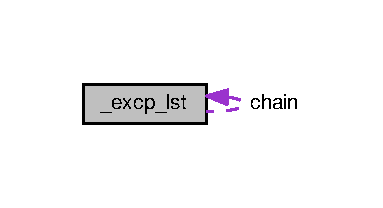
\includegraphics[width=184pt]{struct__excp__lst__coll__graph}
\end{center}
\end{figure}
\subsection*{Data Fields}
\begin{DoxyCompactItemize}
\item 
struct \hyperlink{struct__excp__lst}{\+\_\+excp\+\_\+lst} $\ast$ \hyperlink{struct__excp__lst_af3aa96f46675863a93c104985a99b44f}{chain}
\item 
E\+X\+C\+E\+P\+T\+I\+O\+N\+\_\+\+D\+I\+S\+P\+O\+S\+I\+T\+I\+ON($\ast$ \hyperlink{struct__excp__lst_a1e1e0c071255497025a22a693efc487c}{handler} )()
\end{DoxyCompactItemize}


\subsection{Field Documentation}
\index{\+\_\+excp\+\_\+lst@{\+\_\+excp\+\_\+lst}!chain@{chain}}
\index{chain@{chain}!\+\_\+excp\+\_\+lst@{\+\_\+excp\+\_\+lst}}
\subsubsection[{\texorpdfstring{chain}{chain}}]{\setlength{\rightskip}{0pt plus 5cm}struct {\bf \+\_\+excp\+\_\+lst}$\ast$ \+\_\+excp\+\_\+lst\+::chain}\hypertarget{struct__excp__lst_af3aa96f46675863a93c104985a99b44f}{}\label{struct__excp__lst_af3aa96f46675863a93c104985a99b44f}
\index{\+\_\+excp\+\_\+lst@{\+\_\+excp\+\_\+lst}!handler@{handler}}
\index{handler@{handler}!\+\_\+excp\+\_\+lst@{\+\_\+excp\+\_\+lst}}
\subsubsection[{\texorpdfstring{handler}{handler}}]{\setlength{\rightskip}{0pt plus 5cm}E\+X\+C\+E\+P\+T\+I\+O\+N\+\_\+\+D\+I\+S\+P\+O\+S\+I\+T\+I\+ON($\ast$ \+\_\+excp\+\_\+lst\+::handler) ()}\hypertarget{struct__excp__lst_a1e1e0c071255497025a22a693efc487c}{}\label{struct__excp__lst_a1e1e0c071255497025a22a693efc487c}


The documentation for this struct was generated from the following file\+:\begin{DoxyCompactItemize}
\item 
gprolog-\/utf8-\/tree/src/\+Engine\+Pl/\hyperlink{WIN32__all__SIGSEGV_8c}{W\+I\+N32\+\_\+all\+\_\+\+S\+I\+G\+S\+E\+G\+V.\+c}\end{DoxyCompactItemize}

\hypertarget{structAliasInf}{}\section{Alias\+Inf Struct Reference}
\label{structAliasInf}\index{Alias\+Inf@{Alias\+Inf}}


{\ttfamily \#include $<$stream\+\_\+supp.\+h$>$}

\subsection*{Data Fields}
\begin{DoxyCompactItemize}
\item 
\hyperlink{gprolog_8h_a4d005b136d7fb28537eb1815f7868b63}{Pl\+Long} \hyperlink{structAliasInf_aa0eddd23c6a16d2a76eecc569dbd34d1}{atom}
\item 
int \hyperlink{structAliasInf_aff64cf68f3f548a6978aa01f8509cc9c}{stm}
\end{DoxyCompactItemize}


\subsection{Field Documentation}
\index{Alias\+Inf@{Alias\+Inf}!atom@{atom}}
\index{atom@{atom}!Alias\+Inf@{Alias\+Inf}}
\subsubsection[{\texorpdfstring{atom}{atom}}]{\setlength{\rightskip}{0pt plus 5cm}{\bf Pl\+Long} Alias\+Inf\+::atom}\hypertarget{structAliasInf_aa0eddd23c6a16d2a76eecc569dbd34d1}{}\label{structAliasInf_aa0eddd23c6a16d2a76eecc569dbd34d1}
\index{Alias\+Inf@{Alias\+Inf}!stm@{stm}}
\index{stm@{stm}!Alias\+Inf@{Alias\+Inf}}
\subsubsection[{\texorpdfstring{stm}{stm}}]{\setlength{\rightskip}{0pt plus 5cm}int Alias\+Inf\+::stm}\hypertarget{structAliasInf_aff64cf68f3f548a6978aa01f8509cc9c}{}\label{structAliasInf_aff64cf68f3f548a6978aa01f8509cc9c}


The documentation for this struct was generated from the following file\+:\begin{DoxyCompactItemize}
\item 
gprolog-\/utf8-\/tree/src/\+Bips\+Pl/\hyperlink{stream__supp_8h}{stream\+\_\+supp.\+h}\end{DoxyCompactItemize}

\hypertarget{structArgInf}{}\section{Arg\+Inf Struct Reference}
\label{structArgInf}\index{Arg\+Inf@{Arg\+Inf}}


{\ttfamily \#include $<$ma\+\_\+parser.\+h$>$}



Collaboration diagram for Arg\+Inf\+:\nopagebreak
\begin{figure}[H]
\begin{center}
\leavevmode
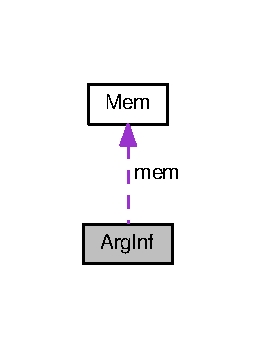
\includegraphics[width=127pt]{structArgInf__coll__graph}
\end{center}
\end{figure}
\subsection*{Data Fields}
\begin{DoxyCompactItemize}
\item 
\hyperlink{ma__parser_8h_a55e83ab108ec469cbb59876c09f146b0}{Arg\+Typ} \hyperlink{structArgInf_ad416abaf87d2e52a23c4d2eb517919e4}{type}
\item 
int \hyperlink{structArgInf_a9a45faac36b5ff6b969faa85446f40e1}{adr\+\_\+of}
\item 
\begin{tabbing}
xx\=xx\=xx\=xx\=xx\=xx\=xx\=xx\=xx\=\kill
union \{\\
\>char $\ast$ \hyperlink{structArgInf_aae189057e919a389c59d0ee897884c5f}{str\_val}\\
\>\hyperlink{gprolog_8h_a4d005b136d7fb28537eb1815f7868b63}{PlLong} \hyperlink{structArgInf_a9b94d186b491b4009a1905f86e41ad9c}{int\_val}\\
\>double \hyperlink{structArgInf_a5ce0eda4a228042bd33b247f80e61144}{dbl\_val}\\
\>\hyperlink{structMem}{Mem} \hyperlink{structArgInf_aa4a2dcaf59861c10d3622f1bdcc5ac3d}{mem}\\
\>int \hyperlink{structArgInf_a053ccdce92762ff8fecd64a3ce561aea}{index}\\
\} \hyperlink{structArgInf_ae7f40cf76bee98b10f0eb3d865b2b912}{t}\\

\end{tabbing}\end{DoxyCompactItemize}


\subsection{Field Documentation}
\index{Arg\+Inf@{Arg\+Inf}!adr\+\_\+of@{adr\+\_\+of}}
\index{adr\+\_\+of@{adr\+\_\+of}!Arg\+Inf@{Arg\+Inf}}
\subsubsection[{\texorpdfstring{adr\+\_\+of}{adr_of}}]{\setlength{\rightskip}{0pt plus 5cm}int Arg\+Inf\+::adr\+\_\+of}\hypertarget{structArgInf_a9a45faac36b5ff6b969faa85446f40e1}{}\label{structArgInf_a9a45faac36b5ff6b969faa85446f40e1}
\index{Arg\+Inf@{Arg\+Inf}!dbl\+\_\+val@{dbl\+\_\+val}}
\index{dbl\+\_\+val@{dbl\+\_\+val}!Arg\+Inf@{Arg\+Inf}}
\subsubsection[{\texorpdfstring{dbl\+\_\+val}{dbl_val}}]{\setlength{\rightskip}{0pt plus 5cm}double Arg\+Inf\+::dbl\+\_\+val}\hypertarget{structArgInf_a5ce0eda4a228042bd33b247f80e61144}{}\label{structArgInf_a5ce0eda4a228042bd33b247f80e61144}
\index{Arg\+Inf@{Arg\+Inf}!index@{index}}
\index{index@{index}!Arg\+Inf@{Arg\+Inf}}
\subsubsection[{\texorpdfstring{index}{index}}]{\setlength{\rightskip}{0pt plus 5cm}int Arg\+Inf\+::index}\hypertarget{structArgInf_a053ccdce92762ff8fecd64a3ce561aea}{}\label{structArgInf_a053ccdce92762ff8fecd64a3ce561aea}
\index{Arg\+Inf@{Arg\+Inf}!int\+\_\+val@{int\+\_\+val}}
\index{int\+\_\+val@{int\+\_\+val}!Arg\+Inf@{Arg\+Inf}}
\subsubsection[{\texorpdfstring{int\+\_\+val}{int_val}}]{\setlength{\rightskip}{0pt plus 5cm}{\bf Pl\+Long} Arg\+Inf\+::int\+\_\+val}\hypertarget{structArgInf_a9b94d186b491b4009a1905f86e41ad9c}{}\label{structArgInf_a9b94d186b491b4009a1905f86e41ad9c}
\index{Arg\+Inf@{Arg\+Inf}!mem@{mem}}
\index{mem@{mem}!Arg\+Inf@{Arg\+Inf}}
\subsubsection[{\texorpdfstring{mem}{mem}}]{\setlength{\rightskip}{0pt plus 5cm}{\bf Mem} Arg\+Inf\+::mem}\hypertarget{structArgInf_aa4a2dcaf59861c10d3622f1bdcc5ac3d}{}\label{structArgInf_aa4a2dcaf59861c10d3622f1bdcc5ac3d}
\index{Arg\+Inf@{Arg\+Inf}!str\+\_\+val@{str\+\_\+val}}
\index{str\+\_\+val@{str\+\_\+val}!Arg\+Inf@{Arg\+Inf}}
\subsubsection[{\texorpdfstring{str\+\_\+val}{str_val}}]{\setlength{\rightskip}{0pt plus 5cm}char$\ast$ Arg\+Inf\+::str\+\_\+val}\hypertarget{structArgInf_aae189057e919a389c59d0ee897884c5f}{}\label{structArgInf_aae189057e919a389c59d0ee897884c5f}
\index{Arg\+Inf@{Arg\+Inf}!t@{t}}
\index{t@{t}!Arg\+Inf@{Arg\+Inf}}
\subsubsection[{\texorpdfstring{t}{t}}]{\setlength{\rightskip}{0pt plus 5cm}union \{ ... \} 
   Arg\+Inf\+::t}\hypertarget{structArgInf_ae7f40cf76bee98b10f0eb3d865b2b912}{}\label{structArgInf_ae7f40cf76bee98b10f0eb3d865b2b912}
\index{Arg\+Inf@{Arg\+Inf}!type@{type}}
\index{type@{type}!Arg\+Inf@{Arg\+Inf}}
\subsubsection[{\texorpdfstring{type}{type}}]{\setlength{\rightskip}{0pt plus 5cm}{\bf Arg\+Typ} Arg\+Inf\+::type}\hypertarget{structArgInf_ad416abaf87d2e52a23c4d2eb517919e4}{}\label{structArgInf_ad416abaf87d2e52a23c4d2eb517919e4}


The documentation for this struct was generated from the following file\+:\begin{DoxyCompactItemize}
\item 
gprolog-\/utf8-\/tree/src/\+Ma2\+Asm/\hyperlink{ma__parser_8h}{ma\+\_\+parser.\+h}\end{DoxyCompactItemize}

\hypertarget{structArithInf}{}\section{Arith\+Inf Struct Reference}
\label{structArithInf}\index{Arith\+Inf@{Arith\+Inf}}
\subsection*{Public Member Functions}
\begin{DoxyCompactItemize}
\item 
\hyperlink{structArithInf_a436fe064b4148705eda3a2a3ed99b067}{Wam\+Word} (\hyperlink{chkma_8c_a46116ed56661a1c5bffe91c80ceae694}{FC} $\ast$\hyperlink{extract__asm_8c_a849db728d9239b130558864aae79168f}{fct})()
\end{DoxyCompactItemize}
\subsection*{Data Fields}
\begin{DoxyCompactItemize}
\item 
\hyperlink{LINUX__SIGSEGV_8c_a10ea8be8823feb38875b8a9326cbb424}{Wam\+Word} \hyperlink{structArithInf_a0adf57977998badbf4fa7d8386fd5bdc}{f\+\_\+n}
\end{DoxyCompactItemize}


\subsection{Member Function Documentation}
\index{Arith\+Inf@{Arith\+Inf}!Wam\+Word@{Wam\+Word}}
\index{Wam\+Word@{Wam\+Word}!Arith\+Inf@{Arith\+Inf}}
\subsubsection[{\texorpdfstring{Wam\+Word(\+F\+C $\ast$fct)()}{WamWord(FC *fct)()}}]{\setlength{\rightskip}{0pt plus 5cm}Arith\+Inf\+::\+Wam\+Word (
\begin{DoxyParamCaption}
\item[{{\bf FC} $\ast$}]{fct}
\end{DoxyParamCaption}
)}\hypertarget{structArithInf_a436fe064b4148705eda3a2a3ed99b067}{}\label{structArithInf_a436fe064b4148705eda3a2a3ed99b067}


\subsection{Field Documentation}
\index{Arith\+Inf@{Arith\+Inf}!f\+\_\+n@{f\+\_\+n}}
\index{f\+\_\+n@{f\+\_\+n}!Arith\+Inf@{Arith\+Inf}}
\subsubsection[{\texorpdfstring{f\+\_\+n}{f_n}}]{\setlength{\rightskip}{0pt plus 5cm}{\bf Wam\+Word} Arith\+Inf\+::f\+\_\+n}\hypertarget{structArithInf_a0adf57977998badbf4fa7d8386fd5bdc}{}\label{structArithInf_a0adf57977998badbf4fa7d8386fd5bdc}


The documentation for this struct was generated from the following file\+:\begin{DoxyCompactItemize}
\item 
gprolog-\/utf8-\/tree/src/\+Bips\+Pl/\hyperlink{arith__inl__c_8c}{arith\+\_\+inl\+\_\+c.\+c}\end{DoxyCompactItemize}

\hypertarget{structAsmLine}{}\section{Asm\+Line Struct Reference}
\label{structAsmLine}\index{Asm\+Line@{Asm\+Line}}
\subsection*{Data Fields}
\begin{DoxyCompactItemize}
\item 
int \hyperlink{structAsmLine_a1b7f8a7f299218d0be5d2e5e15bb974e}{label}
\item 
char \hyperlink{structAsmLine_af94ff4cc2a4abfdf5eed77061fd34f68}{code\+\_\+op} \mbox{[}32\mbox{]}
\item 
char \hyperlink{structAsmLine_a77453b03d07a24336adf4f62b5bbc9c8}{args} \mbox{[}256\mbox{]}
\end{DoxyCompactItemize}


\subsection{Field Documentation}
\index{Asm\+Line@{Asm\+Line}!args@{args}}
\index{args@{args}!Asm\+Line@{Asm\+Line}}
\subsubsection[{\texorpdfstring{args}{args}}]{\setlength{\rightskip}{0pt plus 5cm}char Asm\+Line\+::args\mbox{[}256\mbox{]}}\hypertarget{structAsmLine_a77453b03d07a24336adf4f62b5bbc9c8}{}\label{structAsmLine_a77453b03d07a24336adf4f62b5bbc9c8}
\index{Asm\+Line@{Asm\+Line}!code\+\_\+op@{code\+\_\+op}}
\index{code\+\_\+op@{code\+\_\+op}!Asm\+Line@{Asm\+Line}}
\subsubsection[{\texorpdfstring{code\+\_\+op}{code_op}}]{\setlength{\rightskip}{0pt plus 5cm}char Asm\+Line\+::code\+\_\+op\mbox{[}32\mbox{]}}\hypertarget{structAsmLine_af94ff4cc2a4abfdf5eed77061fd34f68}{}\label{structAsmLine_af94ff4cc2a4abfdf5eed77061fd34f68}
\index{Asm\+Line@{Asm\+Line}!label@{label}}
\index{label@{label}!Asm\+Line@{Asm\+Line}}
\subsubsection[{\texorpdfstring{label}{label}}]{\setlength{\rightskip}{0pt plus 5cm}int Asm\+Line\+::label}\hypertarget{structAsmLine_a1b7f8a7f299218d0be5d2e5e15bb974e}{}\label{structAsmLine_a1b7f8a7f299218d0be5d2e5e15bb974e}


The documentation for this struct was generated from the following file\+:\begin{DoxyCompactItemize}
\item 
gprolog-\/utf8-\/tree/src/\+Ma2\+Asm/\hyperlink{extract__asm_8c}{extract\+\_\+asm.\+c}\end{DoxyCompactItemize}

\hypertarget{structAtomInf}{}\section{Atom\+Inf Struct Reference}
\label{structAtomInf}\index{Atom\+Inf@{Atom\+Inf}}


{\ttfamily \#include $<$atom.\+h$>$}



Collaboration diagram for Atom\+Inf\+:\nopagebreak
\begin{figure}[H]
\begin{center}
\leavevmode
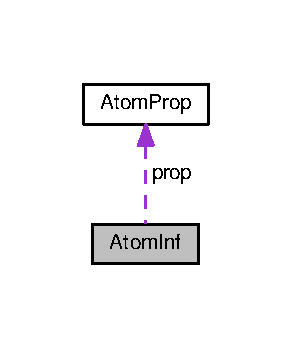
\includegraphics[width=140pt]{structAtomInf__coll__graph}
\end{center}
\end{figure}
\subsection*{Data Fields}
\begin{DoxyCompactItemize}
\item 
char $\ast$ \hyperlink{structAtomInf_a2e8fbcd0d525d43b562f771d099e694e}{name}
\item 
unsigned \hyperlink{structAtomInf_aa2294890b36422410177f1ac258c5157}{hash}
\item 
\hyperlink{structAtomProp}{Atom\+Prop} \hyperlink{structAtomInf_a649620e4716f966372c391e2e8e5245d}{prop}
\item 
void $\ast$ \hyperlink{structAtomInf_a497dcae4cea5b3a779731b97476d05a5}{info}
\end{DoxyCompactItemize}


\subsection{Field Documentation}
\index{Atom\+Inf@{Atom\+Inf}!hash@{hash}}
\index{hash@{hash}!Atom\+Inf@{Atom\+Inf}}
\subsubsection[{\texorpdfstring{hash}{hash}}]{\setlength{\rightskip}{0pt plus 5cm}unsigned Atom\+Inf\+::hash}\hypertarget{structAtomInf_aa2294890b36422410177f1ac258c5157}{}\label{structAtomInf_aa2294890b36422410177f1ac258c5157}
\index{Atom\+Inf@{Atom\+Inf}!info@{info}}
\index{info@{info}!Atom\+Inf@{Atom\+Inf}}
\subsubsection[{\texorpdfstring{info}{info}}]{\setlength{\rightskip}{0pt plus 5cm}void$\ast$ Atom\+Inf\+::info}\hypertarget{structAtomInf_a497dcae4cea5b3a779731b97476d05a5}{}\label{structAtomInf_a497dcae4cea5b3a779731b97476d05a5}
\index{Atom\+Inf@{Atom\+Inf}!name@{name}}
\index{name@{name}!Atom\+Inf@{Atom\+Inf}}
\subsubsection[{\texorpdfstring{name}{name}}]{\setlength{\rightskip}{0pt plus 5cm}char$\ast$ Atom\+Inf\+::name}\hypertarget{structAtomInf_a2e8fbcd0d525d43b562f771d099e694e}{}\label{structAtomInf_a2e8fbcd0d525d43b562f771d099e694e}
\index{Atom\+Inf@{Atom\+Inf}!prop@{prop}}
\index{prop@{prop}!Atom\+Inf@{Atom\+Inf}}
\subsubsection[{\texorpdfstring{prop}{prop}}]{\setlength{\rightskip}{0pt plus 5cm}{\bf Atom\+Prop} Atom\+Inf\+::prop}\hypertarget{structAtomInf_a649620e4716f966372c391e2e8e5245d}{}\label{structAtomInf_a649620e4716f966372c391e2e8e5245d}


The documentation for this struct was generated from the following file\+:\begin{DoxyCompactItemize}
\item 
gprolog-\/utf8-\/tree/src/\+Engine\+Pl/\hyperlink{atom_8h}{atom.\+h}\end{DoxyCompactItemize}

\hypertarget{structAtomProp}{}\section{Atom\+Prop Struct Reference}
\label{structAtomProp}\index{Atom\+Prop@{Atom\+Prop}}
\subsection*{Data Fields}
\begin{DoxyCompactItemize}
\item 
unsigned {\bfseries length}\+:16\hypertarget{structAtomProp_a5708a8e58126cdcd641e6c24e7dd429d}{}\label{structAtomProp_a5708a8e58126cdcd641e6c24e7dd429d}

\item 
unsigned {\bfseries count}\+:16\hypertarget{structAtomProp_a686f0165443645d420bfd7381ddfedb0}{}\label{structAtomProp_a686f0165443645d420bfd7381ddfedb0}

\item 
unsigned {\bfseries op\+\_\+mask}\+:4\hypertarget{structAtomProp_add308662f264e390f71e5557b97837c0}{}\label{structAtomProp_add308662f264e390f71e5557b97837c0}

\item 
unsigned {\bfseries type}\+:2\hypertarget{structAtomProp_accd017afa6f2854bb9316f492449c025}{}\label{structAtomProp_accd017afa6f2854bb9316f492449c025}

\item 
unsigned {\bfseries needs\+\_\+quote}\+:1\hypertarget{structAtomProp_a4b3fe8dfeb73dc67be63684028709774}{}\label{structAtomProp_a4b3fe8dfeb73dc67be63684028709774}

\item 
unsigned {\bfseries needs\+\_\+scan}\+:1\hypertarget{structAtomProp_ada3d42fc8a9d6e708de7db347444b6ee}{}\label{structAtomProp_ada3d42fc8a9d6e708de7db347444b6ee}

\end{DoxyCompactItemize}


The documentation for this struct was generated from the following file\+:\begin{DoxyCompactItemize}
\item 
gprolog-\/utf8-\/tree/src/\+Engine\+Pl/atom.\+h\end{DoxyCompactItemize}

\hypertarget{unionBCWord}{}\section{B\+C\+Word Union Reference}
\label{unionBCWord}\index{B\+C\+Word@{B\+C\+Word}}
\subsection*{Data Fields}
\begin{DoxyCompactItemize}
\item 
\begin{tabbing}
xx\=xx\=xx\=xx\=xx\=xx\=xx\=xx\=xx\=\kill
struct \{\\
\>unsigned {\bfseries code\_op}:8\\
\>unsigned {\bfseries i8}:8\\
\>unsigned {\bfseries i16}:16\\
\} {\bfseries t1}\hypertarget{unionBCWord_a70e755edbb220fd93df2c19803233c99}{}\label{unionBCWord_a70e755edbb220fd93df2c19803233c99}
\\

\end{tabbing}\item 
\begin{tabbing}
xx\=xx\=xx\=xx\=xx\=xx\=xx\=xx\=xx\=\kill
struct \{\\
\>unsigned {\bfseries code\_op}:8\\
\>unsigned {\bfseries i24}:24\\
\} {\bfseries t2}\hypertarget{unionBCWord_abbf0ee87987d69cb8a46e49454401f7c}{}\label{unionBCWord_abbf0ee87987d69cb8a46e49454401f7c}
\\

\end{tabbing}\item 
unsigned {\bfseries word}\hypertarget{unionBCWord_ae6b64a6557710fc6e57ebbd02d1a3bc1}{}\label{unionBCWord_ae6b64a6557710fc6e57ebbd02d1a3bc1}

\end{DoxyCompactItemize}


The documentation for this union was generated from the following file\+:\begin{DoxyCompactItemize}
\item 
gprolog-\/utf8-\/tree/src/\+Bips\+Pl/bc\+\_\+supp.\+c\end{DoxyCompactItemize}

\hypertarget{structbtnode}{}\section{btnode Struct Reference}
\label{structbtnode}\index{btnode@{btnode}}


Collaboration diagram for btnode\+:\nopagebreak
\begin{figure}[H]
\begin{center}
\leavevmode
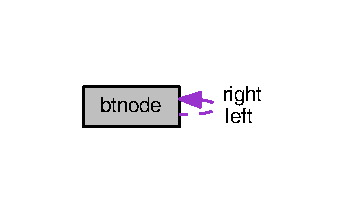
\includegraphics[width=166pt]{structbtnode__coll__graph}
\end{center}
\end{figure}
\subsection*{Data Fields}
\begin{DoxyCompactItemize}
\item 
char $\ast$ {\bfseries str}\hypertarget{structbtnode_ad3235a44ef495ead7832dc7242184d3b}{}\label{structbtnode_ad3235a44ef495ead7832dc7242184d3b}

\item 
int {\bfseries no}\hypertarget{structbtnode_ae1befed4e49931603b1a62f760242f52}{}\label{structbtnode_ae1befed4e49931603b1a62f760242f52}

\item 
char {\bfseries info} \mbox{[}32\mbox{]}\hypertarget{structbtnode_a822bfc05cc3514c5d2799f66c65112e8}{}\label{structbtnode_a822bfc05cc3514c5d2799f66c65112e8}

\item 
\hyperlink{structbtnode}{P\+B\+T\+Node} {\bfseries left}\hypertarget{structbtnode_a595372884aee31dd6b91ba5400f98794}{}\label{structbtnode_a595372884aee31dd6b91ba5400f98794}

\item 
\hyperlink{structbtnode}{P\+B\+T\+Node} {\bfseries right}\hypertarget{structbtnode_a5a315554fa5e275f6f505e94135b1cf4}{}\label{structbtnode_a5a315554fa5e275f6f505e94135b1cf4}

\end{DoxyCompactItemize}


The documentation for this struct was generated from the following file\+:\begin{DoxyCompactItemize}
\item 
gprolog-\/utf8-\/tree/src/\+Wam2\+Ma/bt\+\_\+string.\+h\end{DoxyCompactItemize}

\hypertarget{structBTString}{}\section{B\+T\+String Struct Reference}
\label{structBTString}\index{B\+T\+String@{B\+T\+String}}


{\ttfamily \#include $<$bt\+\_\+string.\+h$>$}



Collaboration diagram for B\+T\+String\+:\nopagebreak
\begin{figure}[H]
\begin{center}
\leavevmode
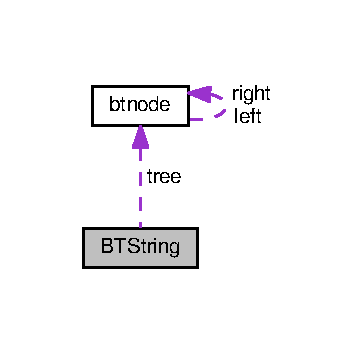
\includegraphics[width=171pt]{structBTString__coll__graph}
\end{center}
\end{figure}
\subsection*{Data Fields}
\begin{DoxyCompactItemize}
\item 
\hyperlink{bt__string_8h_a94e2311ccccb66fae2c4ce55649526fc}{B\+T\+Node} $\ast$ \hyperlink{structBTString_a3d5e702b03b4afc55252841d531836f8}{tree}
\item 
int \hyperlink{structBTString_a4248622c60ccba995140069c3c1fa116}{nb\+\_\+elem}
\end{DoxyCompactItemize}


\subsection{Field Documentation}
\index{B\+T\+String@{B\+T\+String}!nb\+\_\+elem@{nb\+\_\+elem}}
\index{nb\+\_\+elem@{nb\+\_\+elem}!B\+T\+String@{B\+T\+String}}
\subsubsection[{\texorpdfstring{nb\+\_\+elem}{nb_elem}}]{\setlength{\rightskip}{0pt plus 5cm}int B\+T\+String\+::nb\+\_\+elem}\hypertarget{structBTString_a4248622c60ccba995140069c3c1fa116}{}\label{structBTString_a4248622c60ccba995140069c3c1fa116}
\index{B\+T\+String@{B\+T\+String}!tree@{tree}}
\index{tree@{tree}!B\+T\+String@{B\+T\+String}}
\subsubsection[{\texorpdfstring{tree}{tree}}]{\setlength{\rightskip}{0pt plus 5cm}{\bf B\+T\+Node}$\ast$ B\+T\+String\+::tree}\hypertarget{structBTString_a3d5e702b03b4afc55252841d531836f8}{}\label{structBTString_a3d5e702b03b4afc55252841d531836f8}


The documentation for this struct was generated from the following file\+:\begin{DoxyCompactItemize}
\item 
gprolog-\/utf8-\/tree/src/\+Wam2\+Ma/\hyperlink{bt__string_8h}{bt\+\_\+string.\+h}\end{DoxyCompactItemize}

\hypertarget{unionC64To32}{}\section{C64\+To32 Union Reference}
\label{unionC64To32}\index{C64\+To32@{C64\+To32}}
\subsection*{Data Fields}
\begin{DoxyCompactItemize}
\item 
double \hyperlink{unionC64To32_a153fec5a65f5557d9e40a57b95ae6dc0}{d}
\item 
unsigned \hyperlink{unionC64To32_aa82ad59db4f982b9779320862ef7f50f}{u} \mbox{[}2\mbox{]}
\end{DoxyCompactItemize}


\subsection{Field Documentation}
\index{C64\+To32@{C64\+To32}!d@{d}}
\index{d@{d}!C64\+To32@{C64\+To32}}
\subsubsection[{\texorpdfstring{d}{d}}]{\setlength{\rightskip}{0pt plus 5cm}double C64\+To32\+::d}\hypertarget{unionC64To32_a153fec5a65f5557d9e40a57b95ae6dc0}{}\label{unionC64To32_a153fec5a65f5557d9e40a57b95ae6dc0}
\index{C64\+To32@{C64\+To32}!u@{u}}
\index{u@{u}!C64\+To32@{C64\+To32}}
\subsubsection[{\texorpdfstring{u}{u}}]{\setlength{\rightskip}{0pt plus 5cm}unsigned C64\+To32\+::u\mbox{[}2\mbox{]}}\hypertarget{unionC64To32_aa82ad59db4f982b9779320862ef7f50f}{}\label{unionC64To32_aa82ad59db4f982b9779320862ef7f50f}


The documentation for this union was generated from the following file\+:\begin{DoxyCompactItemize}
\item 
gprolog-\/utf8-\/tree/src/\+Bips\+Pl/\hyperlink{bc__supp_8c}{bc\+\_\+supp.\+c}\end{DoxyCompactItemize}

\hypertarget{structCmdInf}{}\section{Cmd\+Inf Struct Reference}
\label{structCmdInf}\index{Cmd\+Inf@{Cmd\+Inf}}
\subsection*{Data Fields}
\begin{DoxyCompactItemize}
\item 
char $\ast$ \hyperlink{structCmdInf_a08f467c4c99d5989d79d571d71eb91cc}{exe\+\_\+name}
\item 
char \hyperlink{structCmdInf_ad3011b5eb07e4f6bc735ba74f0061fb5}{opt} \mbox{[}\hyperlink{top__comp_8c_a3be28e77218549701fd7677b5d2d8b4b}{C\+M\+D\+\_\+\+L\+I\+N\+E\+\_\+\+M\+A\+X\+\_\+\+O\+PT}\mbox{]}
\item 
char $\ast$ \hyperlink{structCmdInf_a8810930cb97bd994d3d5a081222e9882}{out\+\_\+opt}
\end{DoxyCompactItemize}


\subsection{Field Documentation}
\index{Cmd\+Inf@{Cmd\+Inf}!exe\+\_\+name@{exe\+\_\+name}}
\index{exe\+\_\+name@{exe\+\_\+name}!Cmd\+Inf@{Cmd\+Inf}}
\subsubsection[{\texorpdfstring{exe\+\_\+name}{exe_name}}]{\setlength{\rightskip}{0pt plus 5cm}char$\ast$ Cmd\+Inf\+::exe\+\_\+name}\hypertarget{structCmdInf_a08f467c4c99d5989d79d571d71eb91cc}{}\label{structCmdInf_a08f467c4c99d5989d79d571d71eb91cc}
\index{Cmd\+Inf@{Cmd\+Inf}!opt@{opt}}
\index{opt@{opt}!Cmd\+Inf@{Cmd\+Inf}}
\subsubsection[{\texorpdfstring{opt}{opt}}]{\setlength{\rightskip}{0pt plus 5cm}char Cmd\+Inf\+::opt\mbox{[}{\bf C\+M\+D\+\_\+\+L\+I\+N\+E\+\_\+\+M\+A\+X\+\_\+\+O\+PT}\mbox{]}}\hypertarget{structCmdInf_ad3011b5eb07e4f6bc735ba74f0061fb5}{}\label{structCmdInf_ad3011b5eb07e4f6bc735ba74f0061fb5}
\index{Cmd\+Inf@{Cmd\+Inf}!out\+\_\+opt@{out\+\_\+opt}}
\index{out\+\_\+opt@{out\+\_\+opt}!Cmd\+Inf@{Cmd\+Inf}}
\subsubsection[{\texorpdfstring{out\+\_\+opt}{out_opt}}]{\setlength{\rightskip}{0pt plus 5cm}char$\ast$ Cmd\+Inf\+::out\+\_\+opt}\hypertarget{structCmdInf_a8810930cb97bd994d3d5a081222e9882}{}\label{structCmdInf_a8810930cb97bd994d3d5a081222e9882}


The documentation for this struct was generated from the following file\+:\begin{DoxyCompactItemize}
\item 
gprolog-\/utf8-\/tree/src/\+Top\+Comp/\hyperlink{top__comp_8c}{top\+\_\+comp.\+c}\end{DoxyCompactItemize}

\hypertarget{structCodeInf}{}\section{Code\+Inf Struct Reference}
\label{structCodeInf}\index{Code\+Inf@{Code\+Inf}}
\subsection*{Data Fields}
\begin{DoxyCompactItemize}
\item 
int {\bfseries prolog}\hypertarget{structCodeInf_a1010280a1eff3f13adae9b219d07c4cb}{}\label{structCodeInf_a1010280a1eff3f13adae9b219d07c4cb}

\item 
int {\bfseries global}\hypertarget{structCodeInf_a0819cfe0da8345734d7e3b6964caf566}{}\label{structCodeInf_a0819cfe0da8345734d7e3b6964caf566}

\end{DoxyCompactItemize}


The documentation for this struct was generated from the following file\+:\begin{DoxyCompactItemize}
\item 
gprolog-\/utf8-\/tree/src/\+Ma2\+Asm/ma2asm.\+c\end{DoxyCompactItemize}

\hypertarget{structcomp__node}{}\section{comp\+\_\+node Struct Reference}
\label{structcomp__node}\index{comp\+\_\+node@{comp\+\_\+node}}


Collaboration diagram for comp\+\_\+node\+:\nopagebreak
\begin{figure}[H]
\begin{center}
\leavevmode
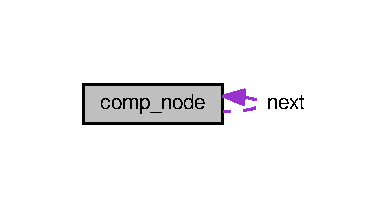
\includegraphics[width=187pt]{structcomp__node__coll__graph}
\end{center}
\end{figure}
\subsection*{Data Fields}
\begin{DoxyCompactItemize}
\item 
char $\ast$ {\bfseries word}\hypertarget{structcomp__node_a087b822f301956dd57ff59bf5d9ce9a4}{}\label{structcomp__node_a087b822f301956dd57ff59bf5d9ce9a4}

\item 
int {\bfseries word\+\_\+length}\hypertarget{structcomp__node_ab0e205b1c196f493851ae425e904c59b}{}\label{structcomp__node_ab0e205b1c196f493851ae425e904c59b}

\item 
\hyperlink{structcomp__node}{Comp\+Node} $\ast$ {\bfseries next}\hypertarget{structcomp__node_aa91fd30c56bcfb19162045c7856d66c8}{}\label{structcomp__node_aa91fd30c56bcfb19162045c7856d66c8}

\end{DoxyCompactItemize}


The documentation for this struct was generated from the following file\+:\begin{DoxyCompactItemize}
\item 
gprolog-\/utf8-\/tree/src/\+Linedit/linedit.\+c\end{DoxyCompactItemize}

\hypertarget{structcptcell}{}\section{cptcell Struct Reference}
\label{structcptcell}\index{cptcell@{cptcell}}


Collaboration diagram for cptcell\+:\nopagebreak
\begin{figure}[H]
\begin{center}
\leavevmode
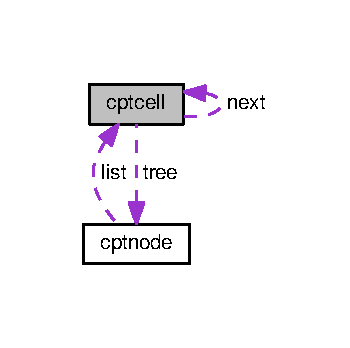
\includegraphics[width=168pt]{structcptcell__coll__graph}
\end{center}
\end{figure}
\subsection*{Data Fields}
\begin{DoxyCompactItemize}
\item 
\hyperlink{cpt__string_8c_ab66488a4813896c44d2e4bbcf8d43a86}{C\+P\+T\+Tree} \hyperlink{structcptcell_a8ce1e2723947c6ebce10520f1fcee6be}{tree}
\item 
\hyperlink{cpt__string_8c_ab32bc138599911e22c2be201414b53e7}{C\+P\+T\+List} \hyperlink{structcptcell_a20fc8bb9280bb623be1dc9e5089df7bb}{next}
\end{DoxyCompactItemize}


\subsection{Field Documentation}
\index{cptcell@{cptcell}!next@{next}}
\index{next@{next}!cptcell@{cptcell}}
\subsubsection[{\texorpdfstring{next}{next}}]{\setlength{\rightskip}{0pt plus 5cm}{\bf C\+P\+T\+List} cptcell\+::next}\hypertarget{structcptcell_a20fc8bb9280bb623be1dc9e5089df7bb}{}\label{structcptcell_a20fc8bb9280bb623be1dc9e5089df7bb}
\index{cptcell@{cptcell}!tree@{tree}}
\index{tree@{tree}!cptcell@{cptcell}}
\subsubsection[{\texorpdfstring{tree}{tree}}]{\setlength{\rightskip}{0pt plus 5cm}{\bf C\+P\+T\+Tree} cptcell\+::tree}\hypertarget{structcptcell_a8ce1e2723947c6ebce10520f1fcee6be}{}\label{structcptcell_a8ce1e2723947c6ebce10520f1fcee6be}


The documentation for this struct was generated from the following file\+:\begin{DoxyCompactItemize}
\item 
gprolog-\/utf8-\/tree/src/\+Engine\+Pl/\hyperlink{cpt__string_8c}{cpt\+\_\+string.\+c}\end{DoxyCompactItemize}

\hypertarget{structCPTMatch}{}\section{C\+P\+T\+Match Struct Reference}
\label{structCPTMatch}\index{C\+P\+T\+Match@{C\+P\+T\+Match}}


Collaboration diagram for C\+P\+T\+Match\+:\nopagebreak
\begin{figure}[H]
\begin{center}
\leavevmode
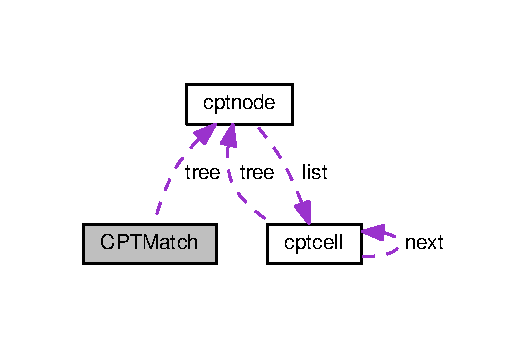
\includegraphics[width=254pt]{structCPTMatch__coll__graph}
\end{center}
\end{figure}
\subsection*{Data Fields}
\begin{DoxyCompactItemize}
\item 
\hyperlink{cpt__string_8c_ab66488a4813896c44d2e4bbcf8d43a86}{C\+P\+T\+Tree} \hyperlink{structCPTMatch_a11fa53acc2fd955cbea152f381e82f31}{tree}
\item 
char $\ast$ \hyperlink{structCPTMatch_a07b32173eb67b2c3e2918bf5a8d29ee5}{buff}
\item 
int \hyperlink{structCPTMatch_aa6d88b8078ed95b080fd648bd46a67c9}{length}
\item 
int($\ast$ \hyperlink{structCPTMatch_a1bee4a76898a1ef5809eb26af9d9673d}{fct} )()
\end{DoxyCompactItemize}


\subsection{Field Documentation}
\index{C\+P\+T\+Match@{C\+P\+T\+Match}!buff@{buff}}
\index{buff@{buff}!C\+P\+T\+Match@{C\+P\+T\+Match}}
\subsubsection[{\texorpdfstring{buff}{buff}}]{\setlength{\rightskip}{0pt plus 5cm}char$\ast$ C\+P\+T\+Match\+::buff}\hypertarget{structCPTMatch_a07b32173eb67b2c3e2918bf5a8d29ee5}{}\label{structCPTMatch_a07b32173eb67b2c3e2918bf5a8d29ee5}
\index{C\+P\+T\+Match@{C\+P\+T\+Match}!fct@{fct}}
\index{fct@{fct}!C\+P\+T\+Match@{C\+P\+T\+Match}}
\subsubsection[{\texorpdfstring{fct}{fct}}]{\setlength{\rightskip}{0pt plus 5cm}int($\ast$ C\+P\+T\+Match\+::fct) ()}\hypertarget{structCPTMatch_a1bee4a76898a1ef5809eb26af9d9673d}{}\label{structCPTMatch_a1bee4a76898a1ef5809eb26af9d9673d}
\index{C\+P\+T\+Match@{C\+P\+T\+Match}!length@{length}}
\index{length@{length}!C\+P\+T\+Match@{C\+P\+T\+Match}}
\subsubsection[{\texorpdfstring{length}{length}}]{\setlength{\rightskip}{0pt plus 5cm}int C\+P\+T\+Match\+::length}\hypertarget{structCPTMatch_aa6d88b8078ed95b080fd648bd46a67c9}{}\label{structCPTMatch_aa6d88b8078ed95b080fd648bd46a67c9}
\index{C\+P\+T\+Match@{C\+P\+T\+Match}!tree@{tree}}
\index{tree@{tree}!C\+P\+T\+Match@{C\+P\+T\+Match}}
\subsubsection[{\texorpdfstring{tree}{tree}}]{\setlength{\rightskip}{0pt plus 5cm}{\bf C\+P\+T\+Tree} C\+P\+T\+Match\+::tree}\hypertarget{structCPTMatch_a11fa53acc2fd955cbea152f381e82f31}{}\label{structCPTMatch_a11fa53acc2fd955cbea152f381e82f31}


The documentation for this struct was generated from the following file\+:\begin{DoxyCompactItemize}
\item 
gprolog-\/utf8-\/tree/src/\+Engine\+Pl/\hyperlink{cpt__string_8c}{cpt\+\_\+string.\+c}\end{DoxyCompactItemize}

\hypertarget{structcptnode}{}\section{cptnode Struct Reference}
\label{structcptnode}\index{cptnode@{cptnode}}


Collaboration diagram for cptnode\+:\nopagebreak
\begin{figure}[H]
\begin{center}
\leavevmode
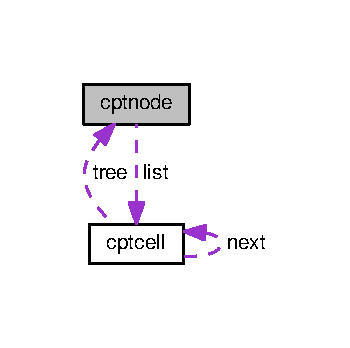
\includegraphics[width=168pt]{structcptnode__coll__graph}
\end{center}
\end{figure}
\subsection*{Data Fields}
\begin{DoxyCompactItemize}
\item 
char $\ast$ \hyperlink{structcptnode_a0f39bf735e3c110c5559c56a2865e3e6}{str}
\item 
int \hyperlink{structcptnode_a18110f6aa5dcbadb7233fb49ee931ee2}{length}
\item 
int \hyperlink{structcptnode_aa3b17740356cb0b60a9bac4f1ee7534d}{end}
\item 
\hyperlink{cpt__string_8c_ab32bc138599911e22c2be201414b53e7}{C\+P\+T\+List} \hyperlink{structcptnode_a957239c445f0b92b306830b91603b8e0}{list}
\end{DoxyCompactItemize}


\subsection{Field Documentation}
\index{cptnode@{cptnode}!end@{end}}
\index{end@{end}!cptnode@{cptnode}}
\subsubsection[{\texorpdfstring{end}{end}}]{\setlength{\rightskip}{0pt plus 5cm}int cptnode\+::end}\hypertarget{structcptnode_aa3b17740356cb0b60a9bac4f1ee7534d}{}\label{structcptnode_aa3b17740356cb0b60a9bac4f1ee7534d}
\index{cptnode@{cptnode}!length@{length}}
\index{length@{length}!cptnode@{cptnode}}
\subsubsection[{\texorpdfstring{length}{length}}]{\setlength{\rightskip}{0pt plus 5cm}int cptnode\+::length}\hypertarget{structcptnode_a18110f6aa5dcbadb7233fb49ee931ee2}{}\label{structcptnode_a18110f6aa5dcbadb7233fb49ee931ee2}
\index{cptnode@{cptnode}!list@{list}}
\index{list@{list}!cptnode@{cptnode}}
\subsubsection[{\texorpdfstring{list}{list}}]{\setlength{\rightskip}{0pt plus 5cm}{\bf C\+P\+T\+List} cptnode\+::list}\hypertarget{structcptnode_a957239c445f0b92b306830b91603b8e0}{}\label{structcptnode_a957239c445f0b92b306830b91603b8e0}
\index{cptnode@{cptnode}!str@{str}}
\index{str@{str}!cptnode@{cptnode}}
\subsubsection[{\texorpdfstring{str}{str}}]{\setlength{\rightskip}{0pt plus 5cm}char$\ast$ cptnode\+::str}\hypertarget{structcptnode_a0f39bf735e3c110c5559c56a2865e3e6}{}\label{structcptnode_a0f39bf735e3c110c5559c56a2865e3e6}


The documentation for this struct was generated from the following file\+:\begin{DoxyCompactItemize}
\item 
gprolog-\/utf8-\/tree/src/\+Engine\+Pl/\hyperlink{cpt__string_8c}{cpt\+\_\+string.\+c}\end{DoxyCompactItemize}

\hypertarget{structCPTStat}{}\section{C\+P\+T\+Stat Struct Reference}
\label{structCPTStat}\index{C\+P\+T\+Stat@{C\+P\+T\+Stat}}
\subsection*{Data Fields}
\begin{DoxyCompactItemize}
\item 
int {\bfseries nb\+\_\+word}\hypertarget{structCPTStat_a58ac2be00efae25c2327d9633b0012d4}{}\label{structCPTStat_a58ac2be00efae25c2327d9633b0012d4}

\item 
int {\bfseries nb\+\_\+node}\hypertarget{structCPTStat_a2fe3f9ca6e2298de8fe583d1998cfa8b}{}\label{structCPTStat_a2fe3f9ca6e2298de8fe583d1998cfa8b}

\item 
int {\bfseries nb\+\_\+node2}\hypertarget{structCPTStat_a1f2b46fe4d9376cb139ac2828467bfce}{}\label{structCPTStat_a1f2b46fe4d9376cb139ac2828467bfce}

\item 
int {\bfseries nb\+\_\+branch}\hypertarget{structCPTStat_af76928968bae2b707f069814504b5045}{}\label{structCPTStat_af76928968bae2b707f069814504b5045}

\item 
int {\bfseries max\+\_\+branch\+\_\+size}\hypertarget{structCPTStat_ae20f9509f4998f41157167b0eb7065b4}{}\label{structCPTStat_ae20f9509f4998f41157167b0eb7065b4}

\item 
int {\bfseries sum\+\_\+branch\+\_\+size\+\_\+word}\hypertarget{structCPTStat_adaea66ddd9de22bf900d0eeeb5486eac}{}\label{structCPTStat_adaea66ddd9de22bf900d0eeeb5486eac}

\item 
int {\bfseries sum\+\_\+branch\+\_\+size}\hypertarget{structCPTStat_a3b3e8fa6689f9725a871430adddf0f30}{}\label{structCPTStat_a3b3e8fa6689f9725a871430adddf0f30}

\item 
int {\bfseries max\+\_\+word\+\_\+length}\hypertarget{structCPTStat_ab03796b9949b9a21fa98a901390ca619}{}\label{structCPTStat_ab03796b9949b9a21fa98a901390ca619}

\item 
int {\bfseries sum\+\_\+word\+\_\+length}\hypertarget{structCPTStat_a8db546c8f4954a69815d75a4ab62a884}{}\label{structCPTStat_a8db546c8f4954a69815d75a4ab62a884}

\item 
int {\bfseries max\+\_\+swrd\+\_\+length}\hypertarget{structCPTStat_a05b16154f6a16eb86044c904c7db9de5}{}\label{structCPTStat_a05b16154f6a16eb86044c904c7db9de5}

\item 
int {\bfseries fst\+\_\+list\+\_\+size}\hypertarget{structCPTStat_aaec7403d2c937e97e1f323b4603d7a17}{}\label{structCPTStat_aaec7403d2c937e97e1f323b4603d7a17}

\item 
int {\bfseries max\+\_\+list\+\_\+size}\hypertarget{structCPTStat_a80e4787886e45e62cff7232be9f4cd7c}{}\label{structCPTStat_a80e4787886e45e62cff7232be9f4cd7c}

\item 
int {\bfseries max2\+\_\+list\+\_\+size}\hypertarget{structCPTStat_acac2689f27927c81da60a96191c99b30}{}\label{structCPTStat_acac2689f27927c81da60a96191c99b30}

\item 
int {\bfseries sum\+\_\+list\+\_\+size}\hypertarget{structCPTStat_ad99f1b443d4a863deb09e79760adf33f}{}\label{structCPTStat_ad99f1b443d4a863deb09e79760adf33f}

\end{DoxyCompactItemize}


The documentation for this struct was generated from the following file\+:\begin{DoxyCompactItemize}
\item 
gprolog-\/utf8-\/tree/src/\+Engine\+Pl/cpt\+\_\+string.\+c\end{DoxyCompactItemize}

\hypertarget{structD2ChCell}{}\section{D2\+Ch\+Cell Struct Reference}
\label{structD2ChCell}\index{D2\+Ch\+Cell@{D2\+Ch\+Cell}}


{\ttfamily \#include $<$dynam\+\_\+supp.\+h$>$}



Collaboration diagram for D2\+Ch\+Cell\+:\nopagebreak
\begin{figure}[H]
\begin{center}
\leavevmode
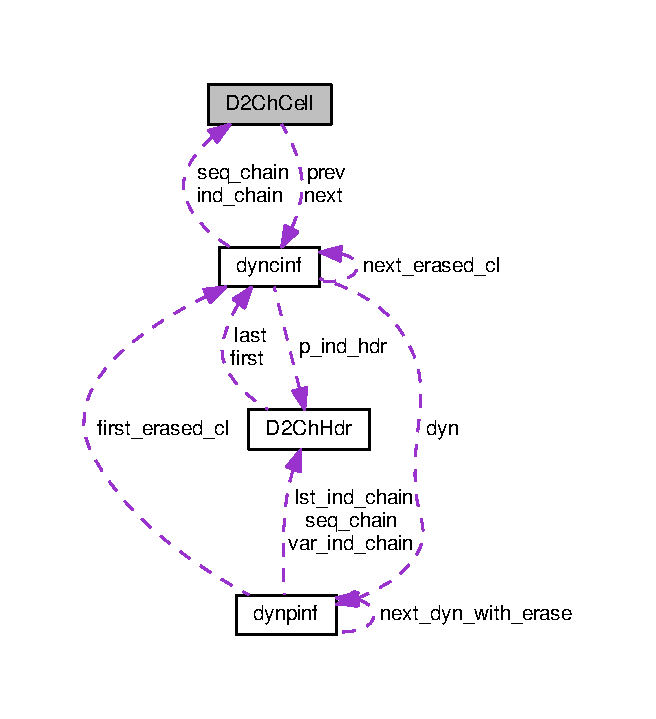
\includegraphics[width=315pt]{structD2ChCell__coll__graph}
\end{center}
\end{figure}
\subsection*{Data Fields}
\begin{DoxyCompactItemize}
\item 
\hyperlink{dynam__supp_8h_ae9665ae9a3ee194834c9995b875aed48}{Dyn\+C\+InfP} \hyperlink{structD2ChCell_ab3eac88c8e41656c4dfa195b314fef5c}{next}
\item 
\hyperlink{dynam__supp_8h_ae9665ae9a3ee194834c9995b875aed48}{Dyn\+C\+InfP} \hyperlink{structD2ChCell_a93c613b80554c6b885b8c680658475cf}{prev}
\end{DoxyCompactItemize}


\subsection{Field Documentation}
\index{D2\+Ch\+Cell@{D2\+Ch\+Cell}!next@{next}}
\index{next@{next}!D2\+Ch\+Cell@{D2\+Ch\+Cell}}
\subsubsection[{\texorpdfstring{next}{next}}]{\setlength{\rightskip}{0pt plus 5cm}{\bf Dyn\+C\+InfP} D2\+Ch\+Cell\+::next}\hypertarget{structD2ChCell_ab3eac88c8e41656c4dfa195b314fef5c}{}\label{structD2ChCell_ab3eac88c8e41656c4dfa195b314fef5c}
\index{D2\+Ch\+Cell@{D2\+Ch\+Cell}!prev@{prev}}
\index{prev@{prev}!D2\+Ch\+Cell@{D2\+Ch\+Cell}}
\subsubsection[{\texorpdfstring{prev}{prev}}]{\setlength{\rightskip}{0pt plus 5cm}{\bf Dyn\+C\+InfP} D2\+Ch\+Cell\+::prev}\hypertarget{structD2ChCell_a93c613b80554c6b885b8c680658475cf}{}\label{structD2ChCell_a93c613b80554c6b885b8c680658475cf}


The documentation for this struct was generated from the following file\+:\begin{DoxyCompactItemize}
\item 
gprolog-\/utf8-\/tree/src/\+Bips\+Pl/\hyperlink{dynam__supp_8h}{dynam\+\_\+supp.\+h}\end{DoxyCompactItemize}

\hypertarget{structD2ChHdr}{}\section{D2\+Ch\+Hdr Struct Reference}
\label{structD2ChHdr}\index{D2\+Ch\+Hdr@{D2\+Ch\+Hdr}}


{\ttfamily \#include $<$dynam\+\_\+supp.\+h$>$}



Collaboration diagram for D2\+Ch\+Hdr\+:\nopagebreak
\begin{figure}[H]
\begin{center}
\leavevmode
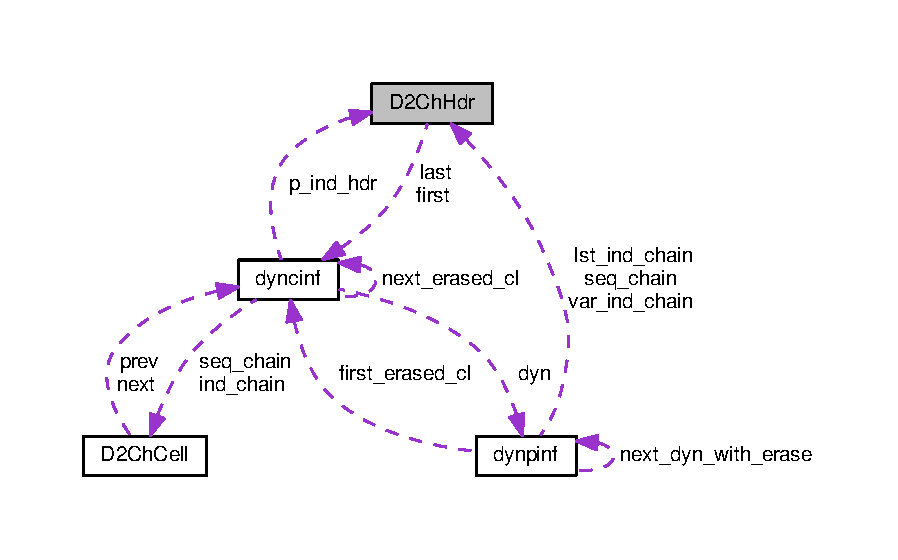
\includegraphics[width=350pt]{structD2ChHdr__coll__graph}
\end{center}
\end{figure}
\subsection*{Data Fields}
\begin{DoxyCompactItemize}
\item 
\hyperlink{dynam__supp_8h_ae9665ae9a3ee194834c9995b875aed48}{Dyn\+C\+InfP} \hyperlink{structD2ChHdr_ac1ff1d6290dd45e018ee4097a2c2427d}{first}
\item 
\hyperlink{dynam__supp_8h_ae9665ae9a3ee194834c9995b875aed48}{Dyn\+C\+InfP} \hyperlink{structD2ChHdr_a35d1cb0c22a72f9a49a6d26b9f8046c8}{last}
\end{DoxyCompactItemize}


\subsection{Field Documentation}
\index{D2\+Ch\+Hdr@{D2\+Ch\+Hdr}!first@{first}}
\index{first@{first}!D2\+Ch\+Hdr@{D2\+Ch\+Hdr}}
\subsubsection[{\texorpdfstring{first}{first}}]{\setlength{\rightskip}{0pt plus 5cm}{\bf Dyn\+C\+InfP} D2\+Ch\+Hdr\+::first}\hypertarget{structD2ChHdr_ac1ff1d6290dd45e018ee4097a2c2427d}{}\label{structD2ChHdr_ac1ff1d6290dd45e018ee4097a2c2427d}
\index{D2\+Ch\+Hdr@{D2\+Ch\+Hdr}!last@{last}}
\index{last@{last}!D2\+Ch\+Hdr@{D2\+Ch\+Hdr}}
\subsubsection[{\texorpdfstring{last}{last}}]{\setlength{\rightskip}{0pt plus 5cm}{\bf Dyn\+C\+InfP} D2\+Ch\+Hdr\+::last}\hypertarget{structD2ChHdr_a35d1cb0c22a72f9a49a6d26b9f8046c8}{}\label{structD2ChHdr_a35d1cb0c22a72f9a49a6d26b9f8046c8}


The documentation for this struct was generated from the following file\+:\begin{DoxyCompactItemize}
\item 
gprolog-\/utf8-\/tree/src/\+Bips\+Pl/\hyperlink{dynam__supp_8h}{dynam\+\_\+supp.\+h}\end{DoxyCompactItemize}

\hypertarget{unionDblInt}{}\section{Dbl\+Int Union Reference}
\label{unionDblInt}\index{Dbl\+Int@{Dbl\+Int}}
\subsection*{Data Fields}
\begin{DoxyCompactItemize}
\item 
double \hyperlink{unionDblInt_a23665c821d8bb2ce3af4f5783fa5ed7c}{d}
\item 
\hyperlink{LINUX__SIGSEGV_8c_a10ea8be8823feb38875b8a9326cbb424}{Wam\+Word} \hyperlink{unionDblInt_ad0ddb3bdd3543a38a19752bc2ac77885}{i} \mbox{[}2\mbox{]}
\end{DoxyCompactItemize}


\subsection{Field Documentation}
\index{Dbl\+Int@{Dbl\+Int}!d@{d}}
\index{d@{d}!Dbl\+Int@{Dbl\+Int}}
\subsubsection[{\texorpdfstring{d}{d}}]{\setlength{\rightskip}{0pt plus 5cm}double Dbl\+Int\+::d}\hypertarget{unionDblInt_a23665c821d8bb2ce3af4f5783fa5ed7c}{}\label{unionDblInt_a23665c821d8bb2ce3af4f5783fa5ed7c}
\index{Dbl\+Int@{Dbl\+Int}!i@{i}}
\index{i@{i}!Dbl\+Int@{Dbl\+Int}}
\subsubsection[{\texorpdfstring{i}{i}}]{\setlength{\rightskip}{0pt plus 5cm}{\bf Wam\+Word} Dbl\+Int\+::i\mbox{[}2\mbox{]}}\hypertarget{unionDblInt_ad0ddb3bdd3543a38a19752bc2ac77885}{}\label{unionDblInt_ad0ddb3bdd3543a38a19752bc2ac77885}


The documentation for this union was generated from the following file\+:\begin{DoxyCompactItemize}
\item 
gprolog-\/utf8-\/tree/src/\+Engine\+Pl/\hyperlink{wam__inst_8c}{wam\+\_\+inst.\+c}\end{DoxyCompactItemize}

\hypertarget{structdirectinf}{}\section{directinf Struct Reference}
\label{structdirectinf}\index{directinf@{directinf}}


Collaboration diagram for directinf\+:\nopagebreak
\begin{figure}[H]
\begin{center}
\leavevmode
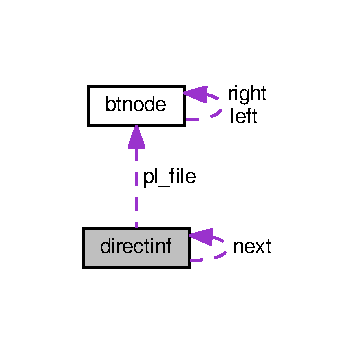
\includegraphics[width=171pt]{structdirectinf__coll__graph}
\end{center}
\end{figure}
\subsection*{Data Fields}
\begin{DoxyCompactItemize}
\item 
\hyperlink{structbtnode}{B\+T\+Node} $\ast$ {\bfseries pl\+\_\+file}\hypertarget{structdirectinf_a2d00b2ef3ca0317b568b16ed20968e52}{}\label{structdirectinf_a2d00b2ef3ca0317b568b16ed20968e52}

\item 
int {\bfseries pl\+\_\+line}\hypertarget{structdirectinf_ae817c137ec2f80b2a6409ae0ca8faa7a}{}\label{structdirectinf_ae817c137ec2f80b2a6409ae0ca8faa7a}

\item 
int {\bfseries system}\hypertarget{structdirectinf_a328d981a0d78b287ff7494df8d501635}{}\label{structdirectinf_a328d981a0d78b287ff7494df8d501635}

\item 
\hyperlink{structdirectinf}{DirectP} {\bfseries next}\hypertarget{structdirectinf_a6376c34c77718e3ea148063383fd29da}{}\label{structdirectinf_a6376c34c77718e3ea148063383fd29da}

\end{DoxyCompactItemize}


The documentation for this struct was generated from the following file\+:\begin{DoxyCompactItemize}
\item 
gprolog-\/utf8-\/tree/src/\+Wam2\+Ma/wam2ma.\+c\end{DoxyCompactItemize}

\hypertarget{structDSwtInf}{}\section{D\+Swt\+Inf Struct Reference}
\label{structDSwtInf}\index{D\+Swt\+Inf@{D\+Swt\+Inf}}


Collaboration diagram for D\+Swt\+Inf\+:\nopagebreak
\begin{figure}[H]
\begin{center}
\leavevmode
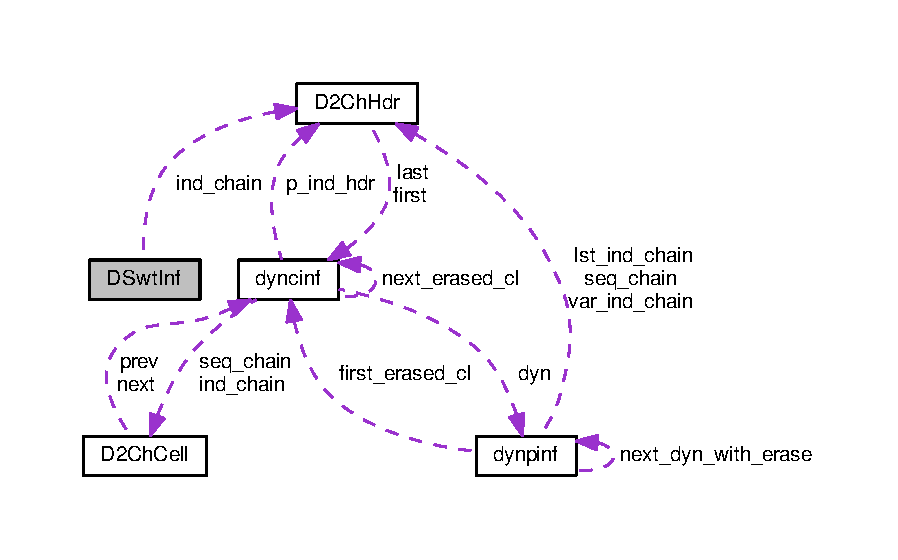
\includegraphics[width=350pt]{structDSwtInf__coll__graph}
\end{center}
\end{figure}
\subsection*{Data Fields}
\begin{DoxyCompactItemize}
\item 
Pl\+Long {\bfseries key}\hypertarget{structDSwtInf_a9661c05b42d3c1c0deb724486fc685b9}{}\label{structDSwtInf_a9661c05b42d3c1c0deb724486fc685b9}

\item 
\hyperlink{structD2ChHdr}{D2\+Ch\+Hdr} {\bfseries ind\+\_\+chain}\hypertarget{structDSwtInf_aa4386ca4933b9847a0622d980023e4c8}{}\label{structDSwtInf_aa4386ca4933b9847a0622d980023e4c8}

\end{DoxyCompactItemize}


The documentation for this struct was generated from the following file\+:\begin{DoxyCompactItemize}
\item 
gprolog-\/utf8-\/tree/src/\+Bips\+Pl/dynam\+\_\+supp.\+h\end{DoxyCompactItemize}

\hypertarget{structdyncinf}{}\section{dyncinf Struct Reference}
\label{structdyncinf}\index{dyncinf@{dyncinf}}


Collaboration diagram for dyncinf\+:\nopagebreak
\begin{figure}[H]
\begin{center}
\leavevmode
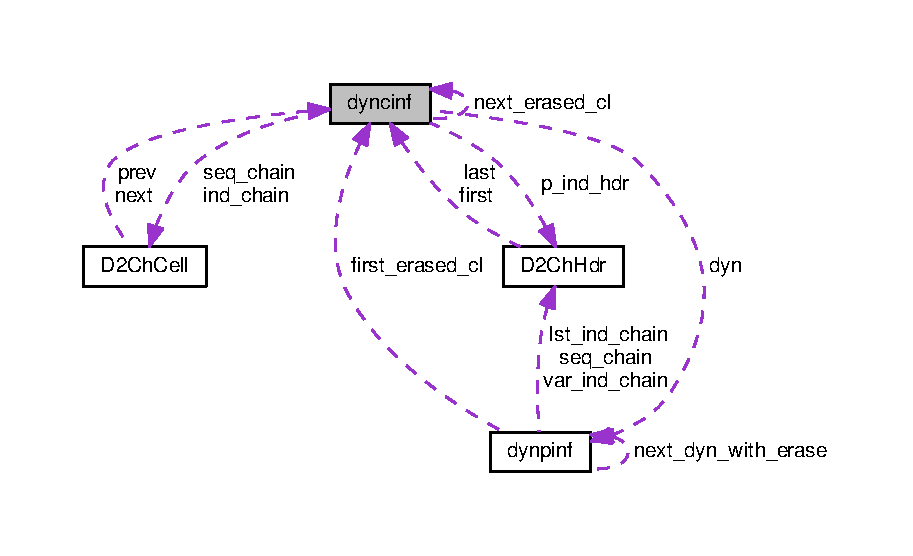
\includegraphics[width=350pt]{structdyncinf__coll__graph}
\end{center}
\end{figure}
\subsection*{Data Fields}
\begin{DoxyCompactItemize}
\item 
\hyperlink{structD2ChCell}{D2\+Ch\+Cell} {\bfseries seq\+\_\+chain}\hypertarget{structdyncinf_a7761fb1d761320cf1779e333348690a1}{}\label{structdyncinf_a7761fb1d761320cf1779e333348690a1}

\item 
\hyperlink{structD2ChCell}{D2\+Ch\+Cell} {\bfseries ind\+\_\+chain}\hypertarget{structdyncinf_a13ff7af2c35333e6fca1f40ab6299a20}{}\label{structdyncinf_a13ff7af2c35333e6fca1f40ab6299a20}

\item 
\hyperlink{structdynpinf}{Dyn\+P\+InfP} {\bfseries dyn}\hypertarget{structdyncinf_a357682e414c932a33d29142f4f3ffc3b}{}\label{structdyncinf_a357682e414c932a33d29142f4f3ffc3b}

\item 
\hyperlink{structD2ChHdr}{D2\+Ch\+Hdr} $\ast$ {\bfseries p\+\_\+ind\+\_\+hdr}\hypertarget{structdyncinf_ad7f2e30b3f0537ad3587209d9f3cc11a}{}\label{structdyncinf_ad7f2e30b3f0537ad3587209d9f3cc11a}

\item 
char $\ast$$\ast$ {\bfseries p\+\_\+ind\+\_\+htbl}\hypertarget{structdyncinf_ac365b7b37b1046432be9fc713bd56ec2}{}\label{structdyncinf_ac365b7b37b1046432be9fc713bd56ec2}

\item 
int {\bfseries cl\+\_\+no}\hypertarget{structdyncinf_a9ecec5cb558eff437ebc9dad0b9a713a}{}\label{structdyncinf_a9ecec5cb558eff437ebc9dad0b9a713a}

\item 
int {\bfseries pl\+\_\+file}\hypertarget{structdyncinf_a8eb75fc2f5558e0fe27a7307dda56f2e}{}\label{structdyncinf_a8eb75fc2f5558e0fe27a7307dda56f2e}

\item 
Dyn\+Stamp {\bfseries erase\+\_\+stamp}\hypertarget{structdyncinf_af4fd2ada2161206351d5d7b462fdf168}{}\label{structdyncinf_af4fd2ada2161206351d5d7b462fdf168}

\item 
\hyperlink{structdyncinf}{Dyn\+C\+InfP} {\bfseries next\+\_\+erased\+\_\+cl}\hypertarget{structdyncinf_a1570173ffbae298cc0c7916bd835f675}{}\label{structdyncinf_a1570173ffbae298cc0c7916bd835f675}

\item 
unsigned $\ast$ {\bfseries byte\+\_\+code}\hypertarget{structdyncinf_a8a16574f97f5162a42cf11f74b16d6b3}{}\label{structdyncinf_a8a16574f97f5162a42cf11f74b16d6b3}

\item 
int {\bfseries term\+\_\+size}\hypertarget{structdyncinf_a4b49c8e104c686701eb19ca0d01173e7}{}\label{structdyncinf_a4b49c8e104c686701eb19ca0d01173e7}

\item 
Wam\+Word {\bfseries term\+\_\+word}\hypertarget{structdyncinf_aad9f2ad962d3ca3002a6fc97dc375d0b}{}\label{structdyncinf_aad9f2ad962d3ca3002a6fc97dc375d0b}

\item 
Wam\+Word {\bfseries head\+\_\+word}\hypertarget{structdyncinf_a11e4b16031cc5023d2f6d2194e328b89}{}\label{structdyncinf_a11e4b16031cc5023d2f6d2194e328b89}

\item 
Wam\+Word {\bfseries body\+\_\+word}\hypertarget{structdyncinf_aaab182b28b71abea34aa78e530aa9483}{}\label{structdyncinf_aaab182b28b71abea34aa78e530aa9483}

\end{DoxyCompactItemize}


The documentation for this struct was generated from the following file\+:\begin{DoxyCompactItemize}
\item 
gprolog-\/utf8-\/tree/src/\+Bips\+Pl/dynam\+\_\+supp.\+h\end{DoxyCompactItemize}

\hypertarget{structdynpinf}{}\section{dynpinf Struct Reference}
\label{structdynpinf}\index{dynpinf@{dynpinf}}


Collaboration diagram for dynpinf\+:\nopagebreak
\begin{figure}[H]
\begin{center}
\leavevmode
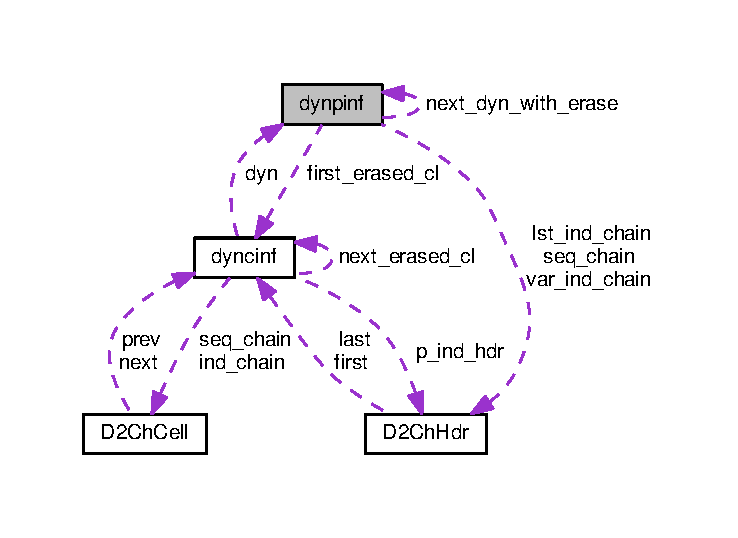
\includegraphics[width=350pt]{structdynpinf__coll__graph}
\end{center}
\end{figure}
\subsection*{Data Fields}
\begin{DoxyCompactItemize}
\item 
\hyperlink{structD2ChHdr}{D2\+Ch\+Hdr} {\bfseries seq\+\_\+chain}\hypertarget{structdynpinf_a7fd9dcc867aa4461a78fd7ea113fe30e}{}\label{structdynpinf_a7fd9dcc867aa4461a78fd7ea113fe30e}

\item 
\hyperlink{structD2ChHdr}{D2\+Ch\+Hdr} {\bfseries var\+\_\+ind\+\_\+chain}\hypertarget{structdynpinf_a81ff1365c770d4e9e503ec13d0829c89}{}\label{structdynpinf_a81ff1365c770d4e9e503ec13d0829c89}

\item 
char $\ast$ {\bfseries atm\+\_\+htbl}\hypertarget{structdynpinf_a647b214d180d3239102e9a3137cd2c50}{}\label{structdynpinf_a647b214d180d3239102e9a3137cd2c50}

\item 
char $\ast$ {\bfseries int\+\_\+htbl}\hypertarget{structdynpinf_a7e89d876755097ac24867ef0c002572d}{}\label{structdynpinf_a7e89d876755097ac24867ef0c002572d}

\item 
\hyperlink{structD2ChHdr}{D2\+Ch\+Hdr} {\bfseries lst\+\_\+ind\+\_\+chain}\hypertarget{structdynpinf_a1c4ab87dddfafc7e912446a2cc391e3f}{}\label{structdynpinf_a1c4ab87dddfafc7e912446a2cc391e3f}

\item 
char $\ast$ {\bfseries stc\+\_\+htbl}\hypertarget{structdynpinf_a34e514b87f630efa4c7d2936979e7735}{}\label{structdynpinf_a34e514b87f630efa4c7d2936979e7735}

\item 
int {\bfseries arity}\hypertarget{structdynpinf_a06c4048e8638d3a47c4b48d5b6384516}{}\label{structdynpinf_a06c4048e8638d3a47c4b48d5b6384516}

\item 
int {\bfseries count\+\_\+a}\hypertarget{structdynpinf_aacc4edd647989f5a014730830390c05d}{}\label{structdynpinf_aacc4edd647989f5a014730830390c05d}

\item 
int {\bfseries count\+\_\+z}\hypertarget{structdynpinf_a90b999f0c08d5d26be5de1f30fd4a83d}{}\label{structdynpinf_a90b999f0c08d5d26be5de1f30fd4a83d}

\item 
\hyperlink{structdyncinf}{Dyn\+C\+InfP} {\bfseries first\+\_\+erased\+\_\+cl}\hypertarget{structdynpinf_a1e974f17af18887bef7754c00313c714}{}\label{structdynpinf_a1e974f17af18887bef7754c00313c714}

\item 
\hyperlink{structdynpinf}{Dyn\+P\+InfP} {\bfseries next\+\_\+dyn\+\_\+with\+\_\+erase}\hypertarget{structdynpinf_a5845421aa8bf227923c6ed1073c32b17}{}\label{structdynpinf_a5845421aa8bf227923c6ed1073c32b17}

\end{DoxyCompactItemize}


The documentation for this struct was generated from the following file\+:\begin{DoxyCompactItemize}
\item 
gprolog-\/utf8-\/tree/src/\+Bips\+Pl/dynam\+\_\+supp.\+h\end{DoxyCompactItemize}

\hypertarget{structDynScan}{}\section{Dyn\+Scan Struct Reference}
\label{structDynScan}\index{Dyn\+Scan@{Dyn\+Scan}}


Collaboration diagram for Dyn\+Scan\+:\nopagebreak
\begin{figure}[H]
\begin{center}
\leavevmode
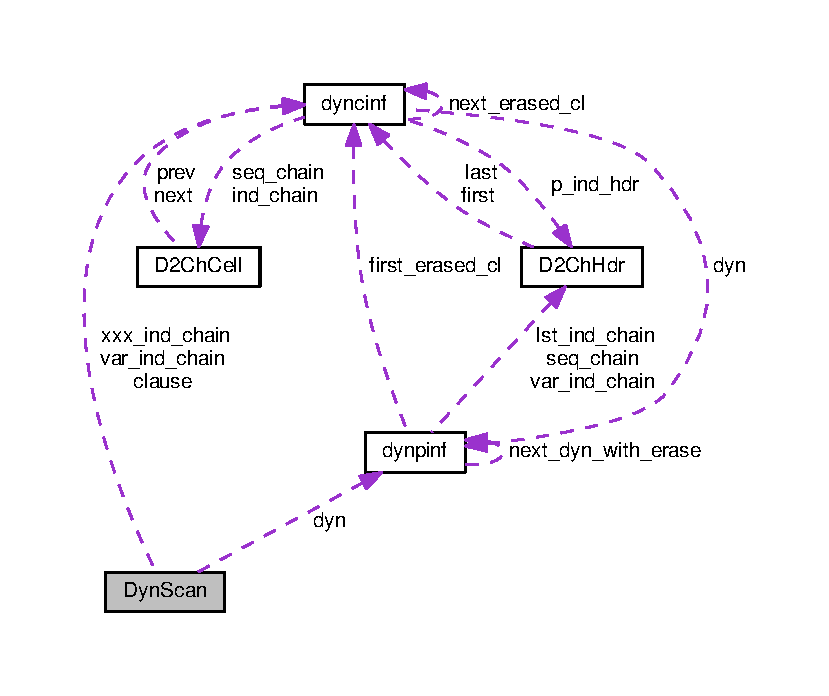
\includegraphics[width=350pt]{structDynScan__coll__graph}
\end{center}
\end{figure}
\subsection*{Data Fields}
\begin{DoxyCompactItemize}
\item 
\hyperlink{dynam__supp_8h_a9ce8f2e1c3c17643fc4a7874b633104e}{Scan\+Fct} \hyperlink{structDynScan_acfa1d047b819d2941ee149649705267a}{alt\+\_\+fct}
\item 
int \hyperlink{structDynScan_add62e7961d11ce60357eb13181e762b0}{alt\+\_\+size\+\_\+info}
\item 
int \hyperlink{structDynScan_a2e6f2cb912f0477854e0cab2bd4f9f0a}{owner\+\_\+func}
\item 
int \hyperlink{structDynScan_a55d99dfd20f733fb1ede548b7accd548}{owner\+\_\+arity}
\item 
\hyperlink{dynam__supp_8h_abf8c639d74e3a538cb5256ede033af03}{Dyn\+P\+Inf} $\ast$ \hyperlink{structDynScan_a2c4d20f447ace62db674692a4724ce0e}{dyn}
\item 
int \hyperlink{structDynScan_a786342f885eab9162a783e6633fefa84}{stop\+\_\+cl\+\_\+no}
\item 
\hyperlink{dynam__supp_8h_ae67d7fd7d828834bf168a2bccc22643c}{Dyn\+Stamp} \hyperlink{structDynScan_a482a71d0fe57d0a6118a68a1f94e0c4a}{erase\+\_\+stamp}
\item 
\hyperlink{bool_8h_afdcfe6db5bea87bd493a3fe2c513d5ef}{Bool} \hyperlink{structDynScan_acd70059e162c998780954a78427ad3ee}{xxx\+\_\+is\+\_\+seq\+\_\+chain}
\item 
\hyperlink{dynam__supp_8h_a3be3c527fb36e120ec36f999fb1a12d3}{Dyn\+C\+Inf} $\ast$ \hyperlink{structDynScan_a657dfdeff11a3a52923f165bcf9bc6fd}{xxx\+\_\+ind\+\_\+chain}
\item 
\hyperlink{dynam__supp_8h_a3be3c527fb36e120ec36f999fb1a12d3}{Dyn\+C\+Inf} $\ast$ \hyperlink{structDynScan_a01058a30b112e62e5768ead8055f6f7f}{var\+\_\+ind\+\_\+chain}
\item 
\hyperlink{dynam__supp_8h_a3be3c527fb36e120ec36f999fb1a12d3}{Dyn\+C\+Inf} $\ast$ \hyperlink{structDynScan_ac04b24fb81aec5128d42e5b79123cfc8}{clause}
\end{DoxyCompactItemize}


\subsection{Field Documentation}
\index{Dyn\+Scan@{Dyn\+Scan}!alt\+\_\+fct@{alt\+\_\+fct}}
\index{alt\+\_\+fct@{alt\+\_\+fct}!Dyn\+Scan@{Dyn\+Scan}}
\subsubsection[{\texorpdfstring{alt\+\_\+fct}{alt_fct}}]{\setlength{\rightskip}{0pt plus 5cm}{\bf Scan\+Fct} Dyn\+Scan\+::alt\+\_\+fct}\hypertarget{structDynScan_acfa1d047b819d2941ee149649705267a}{}\label{structDynScan_acfa1d047b819d2941ee149649705267a}
\index{Dyn\+Scan@{Dyn\+Scan}!alt\+\_\+size\+\_\+info@{alt\+\_\+size\+\_\+info}}
\index{alt\+\_\+size\+\_\+info@{alt\+\_\+size\+\_\+info}!Dyn\+Scan@{Dyn\+Scan}}
\subsubsection[{\texorpdfstring{alt\+\_\+size\+\_\+info}{alt_size_info}}]{\setlength{\rightskip}{0pt plus 5cm}int Dyn\+Scan\+::alt\+\_\+size\+\_\+info}\hypertarget{structDynScan_add62e7961d11ce60357eb13181e762b0}{}\label{structDynScan_add62e7961d11ce60357eb13181e762b0}
\index{Dyn\+Scan@{Dyn\+Scan}!clause@{clause}}
\index{clause@{clause}!Dyn\+Scan@{Dyn\+Scan}}
\subsubsection[{\texorpdfstring{clause}{clause}}]{\setlength{\rightskip}{0pt plus 5cm}{\bf Dyn\+C\+Inf}$\ast$ Dyn\+Scan\+::clause}\hypertarget{structDynScan_ac04b24fb81aec5128d42e5b79123cfc8}{}\label{structDynScan_ac04b24fb81aec5128d42e5b79123cfc8}
\index{Dyn\+Scan@{Dyn\+Scan}!dyn@{dyn}}
\index{dyn@{dyn}!Dyn\+Scan@{Dyn\+Scan}}
\subsubsection[{\texorpdfstring{dyn}{dyn}}]{\setlength{\rightskip}{0pt plus 5cm}{\bf Dyn\+P\+Inf}$\ast$ Dyn\+Scan\+::dyn}\hypertarget{structDynScan_a2c4d20f447ace62db674692a4724ce0e}{}\label{structDynScan_a2c4d20f447ace62db674692a4724ce0e}
\index{Dyn\+Scan@{Dyn\+Scan}!erase\+\_\+stamp@{erase\+\_\+stamp}}
\index{erase\+\_\+stamp@{erase\+\_\+stamp}!Dyn\+Scan@{Dyn\+Scan}}
\subsubsection[{\texorpdfstring{erase\+\_\+stamp}{erase_stamp}}]{\setlength{\rightskip}{0pt plus 5cm}{\bf Dyn\+Stamp} Dyn\+Scan\+::erase\+\_\+stamp}\hypertarget{structDynScan_a482a71d0fe57d0a6118a68a1f94e0c4a}{}\label{structDynScan_a482a71d0fe57d0a6118a68a1f94e0c4a}
\index{Dyn\+Scan@{Dyn\+Scan}!owner\+\_\+arity@{owner\+\_\+arity}}
\index{owner\+\_\+arity@{owner\+\_\+arity}!Dyn\+Scan@{Dyn\+Scan}}
\subsubsection[{\texorpdfstring{owner\+\_\+arity}{owner_arity}}]{\setlength{\rightskip}{0pt plus 5cm}int Dyn\+Scan\+::owner\+\_\+arity}\hypertarget{structDynScan_a55d99dfd20f733fb1ede548b7accd548}{}\label{structDynScan_a55d99dfd20f733fb1ede548b7accd548}
\index{Dyn\+Scan@{Dyn\+Scan}!owner\+\_\+func@{owner\+\_\+func}}
\index{owner\+\_\+func@{owner\+\_\+func}!Dyn\+Scan@{Dyn\+Scan}}
\subsubsection[{\texorpdfstring{owner\+\_\+func}{owner_func}}]{\setlength{\rightskip}{0pt plus 5cm}int Dyn\+Scan\+::owner\+\_\+func}\hypertarget{structDynScan_a2e6f2cb912f0477854e0cab2bd4f9f0a}{}\label{structDynScan_a2e6f2cb912f0477854e0cab2bd4f9f0a}
\index{Dyn\+Scan@{Dyn\+Scan}!stop\+\_\+cl\+\_\+no@{stop\+\_\+cl\+\_\+no}}
\index{stop\+\_\+cl\+\_\+no@{stop\+\_\+cl\+\_\+no}!Dyn\+Scan@{Dyn\+Scan}}
\subsubsection[{\texorpdfstring{stop\+\_\+cl\+\_\+no}{stop_cl_no}}]{\setlength{\rightskip}{0pt plus 5cm}int Dyn\+Scan\+::stop\+\_\+cl\+\_\+no}\hypertarget{structDynScan_a786342f885eab9162a783e6633fefa84}{}\label{structDynScan_a786342f885eab9162a783e6633fefa84}
\index{Dyn\+Scan@{Dyn\+Scan}!var\+\_\+ind\+\_\+chain@{var\+\_\+ind\+\_\+chain}}
\index{var\+\_\+ind\+\_\+chain@{var\+\_\+ind\+\_\+chain}!Dyn\+Scan@{Dyn\+Scan}}
\subsubsection[{\texorpdfstring{var\+\_\+ind\+\_\+chain}{var_ind_chain}}]{\setlength{\rightskip}{0pt plus 5cm}{\bf Dyn\+C\+Inf}$\ast$ Dyn\+Scan\+::var\+\_\+ind\+\_\+chain}\hypertarget{structDynScan_a01058a30b112e62e5768ead8055f6f7f}{}\label{structDynScan_a01058a30b112e62e5768ead8055f6f7f}
\index{Dyn\+Scan@{Dyn\+Scan}!xxx\+\_\+ind\+\_\+chain@{xxx\+\_\+ind\+\_\+chain}}
\index{xxx\+\_\+ind\+\_\+chain@{xxx\+\_\+ind\+\_\+chain}!Dyn\+Scan@{Dyn\+Scan}}
\subsubsection[{\texorpdfstring{xxx\+\_\+ind\+\_\+chain}{xxx_ind_chain}}]{\setlength{\rightskip}{0pt plus 5cm}{\bf Dyn\+C\+Inf}$\ast$ Dyn\+Scan\+::xxx\+\_\+ind\+\_\+chain}\hypertarget{structDynScan_a657dfdeff11a3a52923f165bcf9bc6fd}{}\label{structDynScan_a657dfdeff11a3a52923f165bcf9bc6fd}
\index{Dyn\+Scan@{Dyn\+Scan}!xxx\+\_\+is\+\_\+seq\+\_\+chain@{xxx\+\_\+is\+\_\+seq\+\_\+chain}}
\index{xxx\+\_\+is\+\_\+seq\+\_\+chain@{xxx\+\_\+is\+\_\+seq\+\_\+chain}!Dyn\+Scan@{Dyn\+Scan}}
\subsubsection[{\texorpdfstring{xxx\+\_\+is\+\_\+seq\+\_\+chain}{xxx_is_seq_chain}}]{\setlength{\rightskip}{0pt plus 5cm}{\bf Bool} Dyn\+Scan\+::xxx\+\_\+is\+\_\+seq\+\_\+chain}\hypertarget{structDynScan_acd70059e162c998780954a78427ad3ee}{}\label{structDynScan_acd70059e162c998780954a78427ad3ee}


The documentation for this struct was generated from the following file\+:\begin{DoxyCompactItemize}
\item 
gprolog-\/utf8-\/tree/src/\+Bips\+Pl/\hyperlink{dynam__supp_8c}{dynam\+\_\+supp.\+c}\end{DoxyCompactItemize}

\hypertarget{structFileInf}{}\section{File\+Inf Struct Reference}
\label{structFileInf}\index{File\+Inf@{File\+Inf}}
\subsection*{Data Fields}
\begin{DoxyCompactItemize}
\item 
char $\ast$ {\bfseries name}\hypertarget{structFileInf_a4dc1b0d5b390f714210d47b147af9e9b}{}\label{structFileInf_a4dc1b0d5b390f714210d47b147af9e9b}

\item 
char $\ast$ {\bfseries suffix}\hypertarget{structFileInf_a5ef754a773b84e5a9917436c6d8afe72}{}\label{structFileInf_a5ef754a773b84e5a9917436c6d8afe72}

\item 
char $\ast$ {\bfseries file\+\_\+part}\hypertarget{structFileInf_acb68ba4e07ba186e94a267560253b2bb}{}\label{structFileInf_acb68ba4e07ba186e94a267560253b2bb}

\item 
int {\bfseries type}\hypertarget{structFileInf_a08c8fec214c452fa67b03a36ac58db5f}{}\label{structFileInf_a08c8fec214c452fa67b03a36ac58db5f}

\item 
char $\ast$ {\bfseries work\+\_\+name1}\hypertarget{structFileInf_aab7c6e078d6f1ae349cf70872f35531d}{}\label{structFileInf_aab7c6e078d6f1ae349cf70872f35531d}

\item 
char $\ast$ {\bfseries work\+\_\+name2}\hypertarget{structFileInf_a73706e94bc2b8654cfba501d8fce856e}{}\label{structFileInf_a73706e94bc2b8654cfba501d8fce856e}

\end{DoxyCompactItemize}


The documentation for this struct was generated from the following file\+:\begin{DoxyCompactItemize}
\item 
gprolog-\/utf8-\/tree/src/\+Top\+Comp/top\+\_\+comp.\+c\end{DoxyCompactItemize}

\hypertarget{structflag__inf}{}\section{flag\+\_\+inf Struct Reference}
\label{structflag__inf}\index{flag\+\_\+inf@{flag\+\_\+inf}}


{\ttfamily \#include $<$flag\+\_\+supp.\+h$>$}



Collaboration diagram for flag\+\_\+inf\+:\nopagebreak
\begin{figure}[H]
\begin{center}
\leavevmode
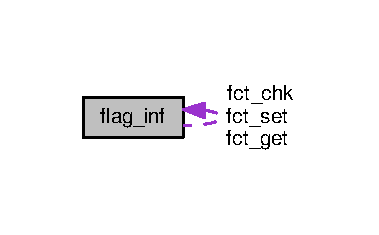
\includegraphics[width=182pt]{structflag__inf__coll__graph}
\end{center}
\end{figure}
\subsection*{Data Fields}
\begin{DoxyCompactItemize}
\item 
int \hyperlink{structflag__inf_a7131c7e545b44d7086d50a89e76bbf30}{atom\+\_\+name}
\item 
\hyperlink{bool_8h_afdcfe6db5bea87bd493a3fe2c513d5ef}{Bool} \hyperlink{structflag__inf_ac95236097fb4811ec47198aa34e64d15}{modifiable}
\item 
\hyperlink{flag__supp_8h_a829563b1e19fae59f905c1afb76fe4eb}{Flag\+Type} \hyperlink{structflag__inf_ad1ffc264915a45e9395b717849c36ff9}{type}
\item 
\hyperlink{gprolog_8h_a4d005b136d7fb28537eb1815f7868b63}{Pl\+Long} \hyperlink{structflag__inf_a828f0d058950ff9e708080d5e96b4068}{value}
\item 
\hyperlink{flag__supp_8h_a54ea5be77d71f1b9cb6e175bea45179c}{Flag\+Fct\+Get} \hyperlink{structflag__inf_ab4585a2020aa37259cb1117664fecfee}{fct\+\_\+get}
\item 
\hyperlink{flag__supp_8h_ac0c2714190598d0ff723cfc7b88b41cd}{Flag\+Fct\+Chk} \hyperlink{structflag__inf_a46997cf1af90c40fa0e2ecee11b935d7}{fct\+\_\+chk}
\item 
\hyperlink{flag__supp_8h_a848a192d7dbb0e8b3715f9322291de21}{Flag\+Fct\+Set} \hyperlink{structflag__inf_aa01403feaa709ffaa582224b5789b928}{fct\+\_\+set}
\end{DoxyCompactItemize}


\subsection{Field Documentation}
\index{flag\+\_\+inf@{flag\+\_\+inf}!atom\+\_\+name@{atom\+\_\+name}}
\index{atom\+\_\+name@{atom\+\_\+name}!flag\+\_\+inf@{flag\+\_\+inf}}
\subsubsection[{\texorpdfstring{atom\+\_\+name}{atom_name}}]{\setlength{\rightskip}{0pt plus 5cm}int flag\+\_\+inf\+::atom\+\_\+name}\hypertarget{structflag__inf_a7131c7e545b44d7086d50a89e76bbf30}{}\label{structflag__inf_a7131c7e545b44d7086d50a89e76bbf30}
\index{flag\+\_\+inf@{flag\+\_\+inf}!fct\+\_\+chk@{fct\+\_\+chk}}
\index{fct\+\_\+chk@{fct\+\_\+chk}!flag\+\_\+inf@{flag\+\_\+inf}}
\subsubsection[{\texorpdfstring{fct\+\_\+chk}{fct_chk}}]{\setlength{\rightskip}{0pt plus 5cm}{\bf Flag\+Fct\+Chk} flag\+\_\+inf\+::fct\+\_\+chk}\hypertarget{structflag__inf_a46997cf1af90c40fa0e2ecee11b935d7}{}\label{structflag__inf_a46997cf1af90c40fa0e2ecee11b935d7}
\index{flag\+\_\+inf@{flag\+\_\+inf}!fct\+\_\+get@{fct\+\_\+get}}
\index{fct\+\_\+get@{fct\+\_\+get}!flag\+\_\+inf@{flag\+\_\+inf}}
\subsubsection[{\texorpdfstring{fct\+\_\+get}{fct_get}}]{\setlength{\rightskip}{0pt plus 5cm}{\bf Flag\+Fct\+Get} flag\+\_\+inf\+::fct\+\_\+get}\hypertarget{structflag__inf_ab4585a2020aa37259cb1117664fecfee}{}\label{structflag__inf_ab4585a2020aa37259cb1117664fecfee}
\index{flag\+\_\+inf@{flag\+\_\+inf}!fct\+\_\+set@{fct\+\_\+set}}
\index{fct\+\_\+set@{fct\+\_\+set}!flag\+\_\+inf@{flag\+\_\+inf}}
\subsubsection[{\texorpdfstring{fct\+\_\+set}{fct_set}}]{\setlength{\rightskip}{0pt plus 5cm}{\bf Flag\+Fct\+Set} flag\+\_\+inf\+::fct\+\_\+set}\hypertarget{structflag__inf_aa01403feaa709ffaa582224b5789b928}{}\label{structflag__inf_aa01403feaa709ffaa582224b5789b928}
\index{flag\+\_\+inf@{flag\+\_\+inf}!modifiable@{modifiable}}
\index{modifiable@{modifiable}!flag\+\_\+inf@{flag\+\_\+inf}}
\subsubsection[{\texorpdfstring{modifiable}{modifiable}}]{\setlength{\rightskip}{0pt plus 5cm}{\bf Bool} flag\+\_\+inf\+::modifiable}\hypertarget{structflag__inf_ac95236097fb4811ec47198aa34e64d15}{}\label{structflag__inf_ac95236097fb4811ec47198aa34e64d15}
\index{flag\+\_\+inf@{flag\+\_\+inf}!type@{type}}
\index{type@{type}!flag\+\_\+inf@{flag\+\_\+inf}}
\subsubsection[{\texorpdfstring{type}{type}}]{\setlength{\rightskip}{0pt plus 5cm}{\bf Flag\+Type} flag\+\_\+inf\+::type}\hypertarget{structflag__inf_ad1ffc264915a45e9395b717849c36ff9}{}\label{structflag__inf_ad1ffc264915a45e9395b717849c36ff9}
\index{flag\+\_\+inf@{flag\+\_\+inf}!value@{value}}
\index{value@{value}!flag\+\_\+inf@{flag\+\_\+inf}}
\subsubsection[{\texorpdfstring{value}{value}}]{\setlength{\rightskip}{0pt plus 5cm}{\bf Pl\+Long} flag\+\_\+inf\+::value}\hypertarget{structflag__inf_a828f0d058950ff9e708080d5e96b4068}{}\label{structflag__inf_a828f0d058950ff9e708080d5e96b4068}


The documentation for this struct was generated from the following file\+:\begin{DoxyCompactItemize}
\item 
gprolog-\/utf8-\/tree/src/\+Bips\+Pl/\hyperlink{flag__supp_8h}{flag\+\_\+supp.\+h}\end{DoxyCompactItemize}

\hypertarget{structGTarget}{}\section{G\+Target Struct Reference}
\label{structGTarget}\index{G\+Target@{G\+Target}}


Collaboration diagram for G\+Target\+:\nopagebreak
\begin{figure}[H]
\begin{center}
\leavevmode
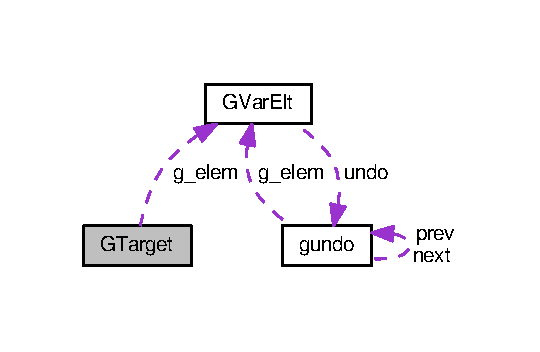
\includegraphics[width=259pt]{structGTarget__coll__graph}
\end{center}
\end{figure}
\subsection*{Data Fields}
\begin{DoxyCompactItemize}
\item 
\hyperlink{structGVarElt}{G\+Var\+Elt} $\ast$ {\bfseries g\+\_\+elem}\hypertarget{structGTarget_a057eea84bfa93fdfb38a7bf7d1bea531}{}\label{structGTarget_a057eea84bfa93fdfb38a7bf7d1bea531}

\item 
Wam\+Word $\ast$ {\bfseries g\+\_\+arg}\hypertarget{structGTarget_a46bf65a569e3ed1e726570e6c0f83a31}{}\label{structGTarget_a46bf65a569e3ed1e726570e6c0f83a31}

\end{DoxyCompactItemize}


The documentation for this struct was generated from the following file\+:\begin{DoxyCompactItemize}
\item 
gprolog-\/utf8-\/tree/src/\+Bips\+Pl/g\+\_\+var\+\_\+inl\+\_\+c.\+c\end{DoxyCompactItemize}

\hypertarget{structgundo}{}\section{gundo Struct Reference}
\label{structgundo}\index{gundo@{gundo}}


Collaboration diagram for gundo\+:\nopagebreak
\begin{figure}[H]
\begin{center}
\leavevmode
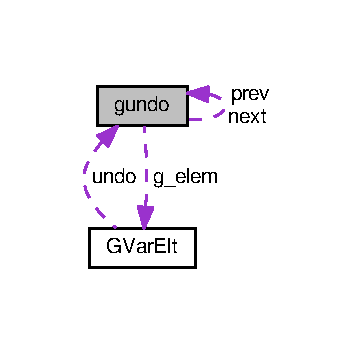
\includegraphics[width=170pt]{structgundo__coll__graph}
\end{center}
\end{figure}
\subsection*{Data Fields}
\begin{DoxyCompactItemize}
\item 
\hyperlink{structGVarElt}{G\+Var\+Elt} $\ast$ {\bfseries g\+\_\+elem}\hypertarget{structgundo_a215f96c167e2bc2aa0902fd04fcce89b}{}\label{structgundo_a215f96c167e2bc2aa0902fd04fcce89b}

\item 
int {\bfseries save\+\_\+size}\hypertarget{structgundo_a543c16d629efbb1e5e1260ef2f9438b5}{}\label{structgundo_a543c16d629efbb1e5e1260ef2f9438b5}

\item 
Wam\+Word {\bfseries save\+\_\+val}\hypertarget{structgundo_ad9b4b183b039fa879a47f9b4a400c742}{}\label{structgundo_ad9b4b183b039fa879a47f9b4a400c742}

\item 
\hyperlink{structgundo}{P\+G\+Undo} {\bfseries next}\hypertarget{structgundo_aa4dd84818a7b36f26b0f7524e850fec9}{}\label{structgundo_aa4dd84818a7b36f26b0f7524e850fec9}

\item 
\hyperlink{structgundo}{P\+G\+Undo} {\bfseries prev}\hypertarget{structgundo_aeb28eb449ba2732d088663c85b986d75}{}\label{structgundo_aeb28eb449ba2732d088663c85b986d75}

\end{DoxyCompactItemize}


The documentation for this struct was generated from the following file\+:\begin{DoxyCompactItemize}
\item 
gprolog-\/utf8-\/tree/src/\+Bips\+Pl/g\+\_\+var\+\_\+inl\+\_\+c.\+c\end{DoxyCompactItemize}

\hypertarget{structGVarElt}{}\section{G\+Var\+Elt Struct Reference}
\label{structGVarElt}\index{G\+Var\+Elt@{G\+Var\+Elt}}


Collaboration diagram for G\+Var\+Elt\+:\nopagebreak
\begin{figure}[H]
\begin{center}
\leavevmode
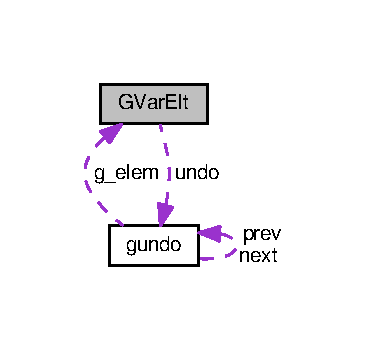
\includegraphics[width=175pt]{structGVarElt__coll__graph}
\end{center}
\end{figure}
\subsection*{Data Fields}
\begin{DoxyCompactItemize}
\item 
int {\bfseries size}\hypertarget{structGVarElt_a34b84647c8816d970311d1a2b3b2fd76}{}\label{structGVarElt_a34b84647c8816d970311d1a2b3b2fd76}

\item 
Wam\+Word {\bfseries val}\hypertarget{structGVarElt_a504e22949f6283a81b42cd76a0016c63}{}\label{structGVarElt_a504e22949f6283a81b42cd76a0016c63}

\item 
\hyperlink{structgundo}{P\+G\+Undo} {\bfseries undo}\hypertarget{structGVarElt_a2c5c97b5670810ddda1590885bdede42}{}\label{structGVarElt_a2c5c97b5670810ddda1590885bdede42}

\end{DoxyCompactItemize}


The documentation for this struct was generated from the following file\+:\begin{DoxyCompactItemize}
\item 
gprolog-\/utf8-\/tree/src/\+Bips\+Pl/g\+\_\+var\+\_\+inl\+\_\+c.\+c\end{DoxyCompactItemize}

\hypertarget{structhash__node}{}\section{hash\+\_\+node Struct Reference}
\label{structhash__node}\index{hash\+\_\+node@{hash\+\_\+node}}


Collaboration diagram for hash\+\_\+node\+:\nopagebreak
\begin{figure}[H]
\begin{center}
\leavevmode
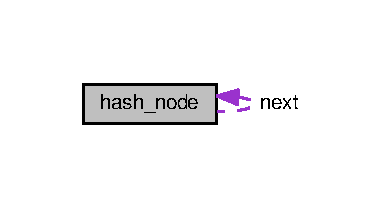
\includegraphics[width=184pt]{structhash__node__coll__graph}
\end{center}
\end{figure}
\subsection*{Data Fields}
\begin{DoxyCompactItemize}
\item 
\hyperlink{structhash__node}{Hash\+Node} {\bfseries next}\hypertarget{structhash__node_a37ad6e543029e7eef401f8be7a984689}{}\label{structhash__node_a37ad6e543029e7eef401f8be7a984689}

\item 
Pl\+Long {\bfseries key}\hypertarget{structhash__node_aa9c0ed0ab7bc110696244024900e9419}{}\label{structhash__node_aa9c0ed0ab7bc110696244024900e9419}

\end{DoxyCompactItemize}


The documentation for this struct was generated from the following file\+:\begin{DoxyCompactItemize}
\item 
gprolog-\/utf8-\/tree/src/\+Engine\+Pl/hash.\+c\end{DoxyCompactItemize}

\hypertarget{structHashIncrInfo}{}\section{Hash\+Incr\+Info Struct Reference}
\label{structHashIncrInfo}\index{Hash\+Incr\+Info@{Hash\+Incr\+Info}}


{\ttfamily \#include $<$hash\+\_\+fct.\+h$>$}

\subsection*{Data Fields}
\begin{DoxyCompactItemize}
\item 
int \hyperlink{structHashIncrInfo_adab7e9365193be88c2bb9e65edbf63bb}{len}
\item 
uint32\+\_\+t \hyperlink{structHashIncrInfo_a3f0d935d1523af0164e99832740c7df7}{hash}
\end{DoxyCompactItemize}


\subsection{Field Documentation}
\index{Hash\+Incr\+Info@{Hash\+Incr\+Info}!hash@{hash}}
\index{hash@{hash}!Hash\+Incr\+Info@{Hash\+Incr\+Info}}
\subsubsection[{\texorpdfstring{hash}{hash}}]{\setlength{\rightskip}{0pt plus 5cm}uint32\+\_\+t Hash\+Incr\+Info\+::hash}\hypertarget{structHashIncrInfo_a3f0d935d1523af0164e99832740c7df7}{}\label{structHashIncrInfo_a3f0d935d1523af0164e99832740c7df7}
\index{Hash\+Incr\+Info@{Hash\+Incr\+Info}!len@{len}}
\index{len@{len}!Hash\+Incr\+Info@{Hash\+Incr\+Info}}
\subsubsection[{\texorpdfstring{len}{len}}]{\setlength{\rightskip}{0pt plus 5cm}int Hash\+Incr\+Info\+::len}\hypertarget{structHashIncrInfo_adab7e9365193be88c2bb9e65edbf63bb}{}\label{structHashIncrInfo_adab7e9365193be88c2bb9e65edbf63bb}


The documentation for this struct was generated from the following file\+:\begin{DoxyCompactItemize}
\item 
gprolog-\/utf8-\/tree/src/\+Engine\+Pl/\hyperlink{hash__fct_8h}{hash\+\_\+fct.\+h}\end{DoxyCompactItemize}

\hypertarget{structHashScan}{}\section{Hash\+Scan Struct Reference}
\label{structHashScan}\index{Hash\+Scan@{Hash\+Scan}}


{\ttfamily \#include $<$hash.\+h$>$}

\subsection*{Data Fields}
\begin{DoxyCompactItemize}
\item 
char $\ast$ \hyperlink{structHashScan_a40b9e0ec1b11cffe3e7bc2c20b7b8a4b}{endt}
\item 
char $\ast$ \hyperlink{structHashScan_af1c9388da5931a00722e2e9ea2c10f42}{cur\+\_\+t}
\item 
char $\ast$ \hyperlink{structHashScan_a267d5612893c8faa728cb27e1edd21aa}{cur\+\_\+p}
\end{DoxyCompactItemize}


\subsection{Field Documentation}
\index{Hash\+Scan@{Hash\+Scan}!cur\+\_\+p@{cur\+\_\+p}}
\index{cur\+\_\+p@{cur\+\_\+p}!Hash\+Scan@{Hash\+Scan}}
\subsubsection[{\texorpdfstring{cur\+\_\+p}{cur_p}}]{\setlength{\rightskip}{0pt plus 5cm}char$\ast$ Hash\+Scan\+::cur\+\_\+p}\hypertarget{structHashScan_a267d5612893c8faa728cb27e1edd21aa}{}\label{structHashScan_a267d5612893c8faa728cb27e1edd21aa}
\index{Hash\+Scan@{Hash\+Scan}!cur\+\_\+t@{cur\+\_\+t}}
\index{cur\+\_\+t@{cur\+\_\+t}!Hash\+Scan@{Hash\+Scan}}
\subsubsection[{\texorpdfstring{cur\+\_\+t}{cur_t}}]{\setlength{\rightskip}{0pt plus 5cm}char$\ast$ Hash\+Scan\+::cur\+\_\+t}\hypertarget{structHashScan_af1c9388da5931a00722e2e9ea2c10f42}{}\label{structHashScan_af1c9388da5931a00722e2e9ea2c10f42}
\index{Hash\+Scan@{Hash\+Scan}!endt@{endt}}
\index{endt@{endt}!Hash\+Scan@{Hash\+Scan}}
\subsubsection[{\texorpdfstring{endt}{endt}}]{\setlength{\rightskip}{0pt plus 5cm}char$\ast$ Hash\+Scan\+::endt}\hypertarget{structHashScan_a40b9e0ec1b11cffe3e7bc2c20b7b8a4b}{}\label{structHashScan_a40b9e0ec1b11cffe3e7bc2c20b7b8a4b}


The documentation for this struct was generated from the following file\+:\begin{DoxyCompactItemize}
\item 
gprolog-\/utf8-\/tree/src/\+Engine\+Pl/\hyperlink{hash_8h}{hash.\+h}\end{DoxyCompactItemize}

\hypertarget{structHistCell}{}\section{Hist\+Cell Struct Reference}
\label{structHistCell}\index{Hist\+Cell@{Hist\+Cell}}
\subsection*{Data Fields}
\begin{DoxyCompactItemize}
\item 
int \hyperlink{structHistCell_a969bc82748a2a5ec09f62d138f62d206}{buff\+\_\+length}
\item 
int \hyperlink{structHistCell_aab32370dee81b023aa2d04e3c6a148e4}{line\+\_\+length}
\item 
char $\ast$ \hyperlink{structHistCell_a7c9560a76c886d7c26f118668303945a}{line}
\end{DoxyCompactItemize}


\subsection{Field Documentation}
\index{Hist\+Cell@{Hist\+Cell}!buff\+\_\+length@{buff\+\_\+length}}
\index{buff\+\_\+length@{buff\+\_\+length}!Hist\+Cell@{Hist\+Cell}}
\subsubsection[{\texorpdfstring{buff\+\_\+length}{buff_length}}]{\setlength{\rightskip}{0pt plus 5cm}int Hist\+Cell\+::buff\+\_\+length}\hypertarget{structHistCell_a969bc82748a2a5ec09f62d138f62d206}{}\label{structHistCell_a969bc82748a2a5ec09f62d138f62d206}
\index{Hist\+Cell@{Hist\+Cell}!line@{line}}
\index{line@{line}!Hist\+Cell@{Hist\+Cell}}
\subsubsection[{\texorpdfstring{line}{line}}]{\setlength{\rightskip}{0pt plus 5cm}char$\ast$ Hist\+Cell\+::line}\hypertarget{structHistCell_a7c9560a76c886d7c26f118668303945a}{}\label{structHistCell_a7c9560a76c886d7c26f118668303945a}
\index{Hist\+Cell@{Hist\+Cell}!line\+\_\+length@{line\+\_\+length}}
\index{line\+\_\+length@{line\+\_\+length}!Hist\+Cell@{Hist\+Cell}}
\subsubsection[{\texorpdfstring{line\+\_\+length}{line_length}}]{\setlength{\rightskip}{0pt plus 5cm}int Hist\+Cell\+::line\+\_\+length}\hypertarget{structHistCell_aab32370dee81b023aa2d04e3c6a148e4}{}\label{structHistCell_aab32370dee81b023aa2d04e3c6a148e4}


The documentation for this struct was generated from the following file\+:\begin{DoxyCompactItemize}
\item 
gprolog-\/utf8-\/tree/src/\+Linedit/\hyperlink{linedit_8c}{linedit.\+c}\end{DoxyCompactItemize}

\hypertarget{structInfCmd}{}\section{Inf\+Cmd Struct Reference}
\label{structInfCmd}\index{Inf\+Cmd@{Inf\+Cmd}}
\subsection*{Data Fields}
\begin{DoxyCompactItemize}
\item 
char $\ast$ {\bfseries name}\hypertarget{structInfCmd_af3fea806d68a1051611b2858d1aa2747}{}\label{structInfCmd_af3fea806d68a1051611b2858d1aa2747}

\item 
Fct\+Ptr {\bfseries fct}\hypertarget{structInfCmd_a4b390073530117560b83be4116a49e0b}{}\label{structInfCmd_a4b390073530117560b83be4116a49e0b}

\end{DoxyCompactItemize}


The documentation for this struct was generated from the following file\+:\begin{DoxyCompactItemize}
\item 
gprolog-\/utf8-\/tree/src/\+Bips\+Pl/debugger\+\_\+c.\+c\end{DoxyCompactItemize}

\hypertarget{structInfSig}{}\section{Inf\+Sig Struct Reference}
\label{structInfSig}\index{Inf\+Sig@{Inf\+Sig}}
\subsection*{Data Fields}
\begin{DoxyCompactItemize}
\item 
int \hyperlink{structInfSig_a802a7fecafff618606688d70860c6ce4}{atom}
\item 
int \hyperlink{structInfSig_a089058351323d661ad411c87017b6647}{sig}
\end{DoxyCompactItemize}


\subsection{Field Documentation}
\index{Inf\+Sig@{Inf\+Sig}!atom@{atom}}
\index{atom@{atom}!Inf\+Sig@{Inf\+Sig}}
\subsubsection[{\texorpdfstring{atom}{atom}}]{\setlength{\rightskip}{0pt plus 5cm}int Inf\+Sig\+::atom}\hypertarget{structInfSig_a802a7fecafff618606688d70860c6ce4}{}\label{structInfSig_a802a7fecafff618606688d70860c6ce4}
\index{Inf\+Sig@{Inf\+Sig}!sig@{sig}}
\index{sig@{sig}!Inf\+Sig@{Inf\+Sig}}
\subsubsection[{\texorpdfstring{sig}{sig}}]{\setlength{\rightskip}{0pt plus 5cm}int Inf\+Sig\+::sig}\hypertarget{structInfSig_a089058351323d661ad411c87017b6647}{}\label{structInfSig_a089058351323d661ad411c87017b6647}


The documentation for this struct was generated from the following file\+:\begin{DoxyCompactItemize}
\item 
gprolog-\/utf8-\/tree/src/\+Bips\+Pl/\hyperlink{os__interf__c_8c}{os\+\_\+interf\+\_\+c.\+c}\end{DoxyCompactItemize}

\hypertarget{structInfVar}{}\section{Inf\+Var Struct Reference}
\label{structInfVar}\index{Inf\+Var@{Inf\+Var}}
\subsection*{Data Fields}
\begin{DoxyCompactItemize}
\item 
char {\bfseries name} \mbox{[}M\+A\+X\+\_\+\+V\+A\+R\+\_\+\+N\+A\+M\+E\+\_\+\+L\+E\+N\+G\+TH\mbox{]}\hypertarget{structInfVar_a0dc32a42fe7338b19884288c0e63b35f}{}\label{structInfVar_a0dc32a42fe7338b19884288c0e63b35f}

\item 
Wam\+Word {\bfseries word}\hypertarget{structInfVar_acc66e228f4cfbb1ab828b0bb95a69621}{}\label{structInfVar_acc66e228f4cfbb1ab828b0bb95a69621}

\item 
Bool {\bfseries named}\hypertarget{structInfVar_a56bb3da1e5f14c34e30d702852740a39}{}\label{structInfVar_a56bb3da1e5f14c34e30d702852740a39}

\item 
int {\bfseries nb\+\_\+of\+\_\+uses}\hypertarget{structInfVar_a38f07afe6ae0ae7f591cf95796469f83}{}\label{structInfVar_a38f07afe6ae0ae7f591cf95796469f83}

\end{DoxyCompactItemize}


The documentation for this struct was generated from the following file\+:\begin{DoxyCompactItemize}
\item 
gprolog-\/utf8-\/tree/src/\+Bips\+Pl/parse\+\_\+supp.\+h\end{DoxyCompactItemize}

\hypertarget{structLongInf}{}\section{Long\+Inf Struct Reference}
\label{structLongInf}\index{Long\+Inf@{Long\+Inf}}
\subsection*{Data Fields}
\begin{DoxyCompactItemize}
\item 
int \hyperlink{structLongInf_a2a21c022832de0f854940c3a39233cec}{global}
\item 
\hyperlink{ma__parser_8h_a28a778aedb7441c6b9755e1882b58dc9}{V\+Type} \hyperlink{structLongInf_a43f3ac657d3dabca28037f16891e4092}{vtype}
\item 
\hyperlink{gprolog_8h_a4d005b136d7fb28537eb1815f7868b63}{Pl\+Long} \hyperlink{structLongInf_ab45336cb32ee695b77f51b6490a81875}{value}
\end{DoxyCompactItemize}


\subsection{Field Documentation}
\index{Long\+Inf@{Long\+Inf}!global@{global}}
\index{global@{global}!Long\+Inf@{Long\+Inf}}
\subsubsection[{\texorpdfstring{global}{global}}]{\setlength{\rightskip}{0pt plus 5cm}int Long\+Inf\+::global}\hypertarget{structLongInf_a2a21c022832de0f854940c3a39233cec}{}\label{structLongInf_a2a21c022832de0f854940c3a39233cec}
\index{Long\+Inf@{Long\+Inf}!value@{value}}
\index{value@{value}!Long\+Inf@{Long\+Inf}}
\subsubsection[{\texorpdfstring{value}{value}}]{\setlength{\rightskip}{0pt plus 5cm}{\bf Pl\+Long} Long\+Inf\+::value}\hypertarget{structLongInf_ab45336cb32ee695b77f51b6490a81875}{}\label{structLongInf_ab45336cb32ee695b77f51b6490a81875}
\index{Long\+Inf@{Long\+Inf}!vtype@{vtype}}
\index{vtype@{vtype}!Long\+Inf@{Long\+Inf}}
\subsubsection[{\texorpdfstring{vtype}{vtype}}]{\setlength{\rightskip}{0pt plus 5cm}{\bf V\+Type} Long\+Inf\+::vtype}\hypertarget{structLongInf_a43f3ac657d3dabca28037f16891e4092}{}\label{structLongInf_a43f3ac657d3dabca28037f16891e4092}


The documentation for this struct was generated from the following file\+:\begin{DoxyCompactItemize}
\item 
gprolog-\/utf8-\/tree/src/\+Ma2\+Asm/\hyperlink{ma2asm_8c}{ma2asm.\+c}\end{DoxyCompactItemize}

\hypertarget{structmallinfo}{}\section{mallinfo Struct Reference}
\label{structmallinfo}\index{mallinfo@{mallinfo}}
\subsection*{Data Fields}
\begin{DoxyCompactItemize}
\item 
\hyperlink{dl__malloc_8c_a53688562ed3d2eda132ae91de874cd98}{M\+A\+L\+L\+I\+N\+F\+O\+\_\+\+F\+I\+E\+L\+D\+\_\+\+T\+Y\+PE} \hyperlink{structmallinfo_a2dd8e574430e788f53919db129f2a2ff}{arena}
\item 
\hyperlink{dl__malloc_8c_a53688562ed3d2eda132ae91de874cd98}{M\+A\+L\+L\+I\+N\+F\+O\+\_\+\+F\+I\+E\+L\+D\+\_\+\+T\+Y\+PE} \hyperlink{structmallinfo_afaac6d1e005097fa1ed835684e23bfa7}{ordblks}
\item 
\hyperlink{dl__malloc_8c_a53688562ed3d2eda132ae91de874cd98}{M\+A\+L\+L\+I\+N\+F\+O\+\_\+\+F\+I\+E\+L\+D\+\_\+\+T\+Y\+PE} \hyperlink{structmallinfo_a93076145f3f542dfe5e4e6d1e3feaf0b}{smblks}
\item 
\hyperlink{dl__malloc_8c_a53688562ed3d2eda132ae91de874cd98}{M\+A\+L\+L\+I\+N\+F\+O\+\_\+\+F\+I\+E\+L\+D\+\_\+\+T\+Y\+PE} \hyperlink{structmallinfo_aaf01c52dcd016834ae176885fa32b550}{hblks}
\item 
\hyperlink{dl__malloc_8c_a53688562ed3d2eda132ae91de874cd98}{M\+A\+L\+L\+I\+N\+F\+O\+\_\+\+F\+I\+E\+L\+D\+\_\+\+T\+Y\+PE} \hyperlink{structmallinfo_ab78bcaeb59449f1a9c292bfe3dde8dbb}{hblkhd}
\item 
\hyperlink{dl__malloc_8c_a53688562ed3d2eda132ae91de874cd98}{M\+A\+L\+L\+I\+N\+F\+O\+\_\+\+F\+I\+E\+L\+D\+\_\+\+T\+Y\+PE} \hyperlink{structmallinfo_a470a5e18a1f5eb3cac48020268ca49b8}{usmblks}
\item 
\hyperlink{dl__malloc_8c_a53688562ed3d2eda132ae91de874cd98}{M\+A\+L\+L\+I\+N\+F\+O\+\_\+\+F\+I\+E\+L\+D\+\_\+\+T\+Y\+PE} \hyperlink{structmallinfo_a6b1a33ff0fc95bdab9c79ce271f58003}{fsmblks}
\item 
\hyperlink{dl__malloc_8c_a53688562ed3d2eda132ae91de874cd98}{M\+A\+L\+L\+I\+N\+F\+O\+\_\+\+F\+I\+E\+L\+D\+\_\+\+T\+Y\+PE} \hyperlink{structmallinfo_a4676f74c10d8bf8b79585b04d520356f}{uordblks}
\item 
\hyperlink{dl__malloc_8c_a53688562ed3d2eda132ae91de874cd98}{M\+A\+L\+L\+I\+N\+F\+O\+\_\+\+F\+I\+E\+L\+D\+\_\+\+T\+Y\+PE} \hyperlink{structmallinfo_a2fc75bf31817d4a64d0a6970aa5278dd}{fordblks}
\item 
\hyperlink{dl__malloc_8c_a53688562ed3d2eda132ae91de874cd98}{M\+A\+L\+L\+I\+N\+F\+O\+\_\+\+F\+I\+E\+L\+D\+\_\+\+T\+Y\+PE} \hyperlink{structmallinfo_a9cd2ce910ff603217426d9b1b7c0e430}{keepcost}
\end{DoxyCompactItemize}


\subsection{Field Documentation}
\index{mallinfo@{mallinfo}!arena@{arena}}
\index{arena@{arena}!mallinfo@{mallinfo}}
\subsubsection[{\texorpdfstring{arena}{arena}}]{\setlength{\rightskip}{0pt plus 5cm}{\bf M\+A\+L\+L\+I\+N\+F\+O\+\_\+\+F\+I\+E\+L\+D\+\_\+\+T\+Y\+PE} mallinfo\+::arena}\hypertarget{structmallinfo_a2dd8e574430e788f53919db129f2a2ff}{}\label{structmallinfo_a2dd8e574430e788f53919db129f2a2ff}
\index{mallinfo@{mallinfo}!fordblks@{fordblks}}
\index{fordblks@{fordblks}!mallinfo@{mallinfo}}
\subsubsection[{\texorpdfstring{fordblks}{fordblks}}]{\setlength{\rightskip}{0pt plus 5cm}{\bf M\+A\+L\+L\+I\+N\+F\+O\+\_\+\+F\+I\+E\+L\+D\+\_\+\+T\+Y\+PE} mallinfo\+::fordblks}\hypertarget{structmallinfo_a2fc75bf31817d4a64d0a6970aa5278dd}{}\label{structmallinfo_a2fc75bf31817d4a64d0a6970aa5278dd}
\index{mallinfo@{mallinfo}!fsmblks@{fsmblks}}
\index{fsmblks@{fsmblks}!mallinfo@{mallinfo}}
\subsubsection[{\texorpdfstring{fsmblks}{fsmblks}}]{\setlength{\rightskip}{0pt plus 5cm}{\bf M\+A\+L\+L\+I\+N\+F\+O\+\_\+\+F\+I\+E\+L\+D\+\_\+\+T\+Y\+PE} mallinfo\+::fsmblks}\hypertarget{structmallinfo_a6b1a33ff0fc95bdab9c79ce271f58003}{}\label{structmallinfo_a6b1a33ff0fc95bdab9c79ce271f58003}
\index{mallinfo@{mallinfo}!hblkhd@{hblkhd}}
\index{hblkhd@{hblkhd}!mallinfo@{mallinfo}}
\subsubsection[{\texorpdfstring{hblkhd}{hblkhd}}]{\setlength{\rightskip}{0pt plus 5cm}{\bf M\+A\+L\+L\+I\+N\+F\+O\+\_\+\+F\+I\+E\+L\+D\+\_\+\+T\+Y\+PE} mallinfo\+::hblkhd}\hypertarget{structmallinfo_ab78bcaeb59449f1a9c292bfe3dde8dbb}{}\label{structmallinfo_ab78bcaeb59449f1a9c292bfe3dde8dbb}
\index{mallinfo@{mallinfo}!hblks@{hblks}}
\index{hblks@{hblks}!mallinfo@{mallinfo}}
\subsubsection[{\texorpdfstring{hblks}{hblks}}]{\setlength{\rightskip}{0pt plus 5cm}{\bf M\+A\+L\+L\+I\+N\+F\+O\+\_\+\+F\+I\+E\+L\+D\+\_\+\+T\+Y\+PE} mallinfo\+::hblks}\hypertarget{structmallinfo_aaf01c52dcd016834ae176885fa32b550}{}\label{structmallinfo_aaf01c52dcd016834ae176885fa32b550}
\index{mallinfo@{mallinfo}!keepcost@{keepcost}}
\index{keepcost@{keepcost}!mallinfo@{mallinfo}}
\subsubsection[{\texorpdfstring{keepcost}{keepcost}}]{\setlength{\rightskip}{0pt plus 5cm}{\bf M\+A\+L\+L\+I\+N\+F\+O\+\_\+\+F\+I\+E\+L\+D\+\_\+\+T\+Y\+PE} mallinfo\+::keepcost}\hypertarget{structmallinfo_a9cd2ce910ff603217426d9b1b7c0e430}{}\label{structmallinfo_a9cd2ce910ff603217426d9b1b7c0e430}
\index{mallinfo@{mallinfo}!ordblks@{ordblks}}
\index{ordblks@{ordblks}!mallinfo@{mallinfo}}
\subsubsection[{\texorpdfstring{ordblks}{ordblks}}]{\setlength{\rightskip}{0pt plus 5cm}{\bf M\+A\+L\+L\+I\+N\+F\+O\+\_\+\+F\+I\+E\+L\+D\+\_\+\+T\+Y\+PE} mallinfo\+::ordblks}\hypertarget{structmallinfo_afaac6d1e005097fa1ed835684e23bfa7}{}\label{structmallinfo_afaac6d1e005097fa1ed835684e23bfa7}
\index{mallinfo@{mallinfo}!smblks@{smblks}}
\index{smblks@{smblks}!mallinfo@{mallinfo}}
\subsubsection[{\texorpdfstring{smblks}{smblks}}]{\setlength{\rightskip}{0pt plus 5cm}{\bf M\+A\+L\+L\+I\+N\+F\+O\+\_\+\+F\+I\+E\+L\+D\+\_\+\+T\+Y\+PE} mallinfo\+::smblks}\hypertarget{structmallinfo_a93076145f3f542dfe5e4e6d1e3feaf0b}{}\label{structmallinfo_a93076145f3f542dfe5e4e6d1e3feaf0b}
\index{mallinfo@{mallinfo}!uordblks@{uordblks}}
\index{uordblks@{uordblks}!mallinfo@{mallinfo}}
\subsubsection[{\texorpdfstring{uordblks}{uordblks}}]{\setlength{\rightskip}{0pt plus 5cm}{\bf M\+A\+L\+L\+I\+N\+F\+O\+\_\+\+F\+I\+E\+L\+D\+\_\+\+T\+Y\+PE} mallinfo\+::uordblks}\hypertarget{structmallinfo_a4676f74c10d8bf8b79585b04d520356f}{}\label{structmallinfo_a4676f74c10d8bf8b79585b04d520356f}
\index{mallinfo@{mallinfo}!usmblks@{usmblks}}
\index{usmblks@{usmblks}!mallinfo@{mallinfo}}
\subsubsection[{\texorpdfstring{usmblks}{usmblks}}]{\setlength{\rightskip}{0pt plus 5cm}{\bf M\+A\+L\+L\+I\+N\+F\+O\+\_\+\+F\+I\+E\+L\+D\+\_\+\+T\+Y\+PE} mallinfo\+::usmblks}\hypertarget{structmallinfo_a470a5e18a1f5eb3cac48020268ca49b8}{}\label{structmallinfo_a470a5e18a1f5eb3cac48020268ca49b8}


The documentation for this struct was generated from the following file\+:\begin{DoxyCompactItemize}
\item 
gprolog-\/utf8-\/tree/src/\+Engine\+Pl/\hyperlink{dl__malloc_8c}{dl\+\_\+malloc.\+c}\end{DoxyCompactItemize}

\hypertarget{structmalloc__chunk}{}\section{malloc\+\_\+chunk Struct Reference}
\label{structmalloc__chunk}\index{malloc\+\_\+chunk@{malloc\+\_\+chunk}}


Collaboration diagram for malloc\+\_\+chunk\+:\nopagebreak
\begin{figure}[H]
\begin{center}
\leavevmode
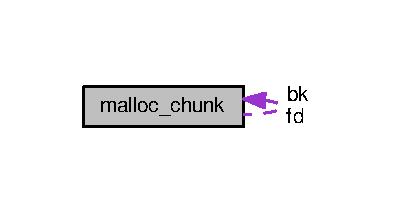
\includegraphics[width=189pt]{structmalloc__chunk__coll__graph}
\end{center}
\end{figure}
\subsection*{Data Fields}
\begin{DoxyCompactItemize}
\item 
size\+\_\+t {\bfseries prev\+\_\+foot}\hypertarget{structmalloc__chunk_a2cbb92874183d7a4b42e150b7d7ec1f9}{}\label{structmalloc__chunk_a2cbb92874183d7a4b42e150b7d7ec1f9}

\item 
size\+\_\+t {\bfseries head}\hypertarget{structmalloc__chunk_a7383bb525d34ca811283c927086205bc}{}\label{structmalloc__chunk_a7383bb525d34ca811283c927086205bc}

\item 
struct \hyperlink{structmalloc__chunk}{malloc\+\_\+chunk} $\ast$ {\bfseries fd}\hypertarget{structmalloc__chunk_a9972ab720231dd0c0d3c202176ce13c5}{}\label{structmalloc__chunk_a9972ab720231dd0c0d3c202176ce13c5}

\item 
struct \hyperlink{structmalloc__chunk}{malloc\+\_\+chunk} $\ast$ {\bfseries bk}\hypertarget{structmalloc__chunk_a268940e08c9c09fc3b2e23cd804bce3c}{}\label{structmalloc__chunk_a268940e08c9c09fc3b2e23cd804bce3c}

\end{DoxyCompactItemize}


The documentation for this struct was generated from the following file\+:\begin{DoxyCompactItemize}
\item 
gprolog-\/utf8-\/tree/src/\+Engine\+Pl/dl\+\_\+malloc.\+c\end{DoxyCompactItemize}

\hypertarget{structmalloc__params}{}\section{malloc\+\_\+params Struct Reference}
\label{structmalloc__params}\index{malloc\+\_\+params@{malloc\+\_\+params}}
\subsection*{Data Fields}
\begin{DoxyCompactItemize}
\item 
size\+\_\+t \hyperlink{structmalloc__params_a7034fc9c71af2cc5ba9cd079effdf5a8}{magic}
\item 
size\+\_\+t \hyperlink{structmalloc__params_a3b7a605d7ebe148a8fb3051465dc3979}{page\+\_\+size}
\item 
size\+\_\+t \hyperlink{structmalloc__params_aa0609453d9ec826c8ffc632cbfb8cf68}{granularity}
\item 
size\+\_\+t \hyperlink{structmalloc__params_a5b2af958efc37d52cfa905bc98b41e1b}{mmap\+\_\+threshold}
\item 
size\+\_\+t \hyperlink{structmalloc__params_accae9b2bcb4df63efcdc0b18826cc578}{trim\+\_\+threshold}
\item 
\hyperlink{dl__malloc_8c_a98d45780d5103f1a6b54a549a3d12de2}{flag\+\_\+t} \hyperlink{structmalloc__params_a0bd6b4819a5d7c629c5ab56262f6296d}{default\+\_\+mflags}
\end{DoxyCompactItemize}


\subsection{Field Documentation}
\index{malloc\+\_\+params@{malloc\+\_\+params}!default\+\_\+mflags@{default\+\_\+mflags}}
\index{default\+\_\+mflags@{default\+\_\+mflags}!malloc\+\_\+params@{malloc\+\_\+params}}
\subsubsection[{\texorpdfstring{default\+\_\+mflags}{default_mflags}}]{\setlength{\rightskip}{0pt plus 5cm}{\bf flag\+\_\+t} malloc\+\_\+params\+::default\+\_\+mflags}\hypertarget{structmalloc__params_a0bd6b4819a5d7c629c5ab56262f6296d}{}\label{structmalloc__params_a0bd6b4819a5d7c629c5ab56262f6296d}
\index{malloc\+\_\+params@{malloc\+\_\+params}!granularity@{granularity}}
\index{granularity@{granularity}!malloc\+\_\+params@{malloc\+\_\+params}}
\subsubsection[{\texorpdfstring{granularity}{granularity}}]{\setlength{\rightskip}{0pt plus 5cm}size\+\_\+t malloc\+\_\+params\+::granularity}\hypertarget{structmalloc__params_aa0609453d9ec826c8ffc632cbfb8cf68}{}\label{structmalloc__params_aa0609453d9ec826c8ffc632cbfb8cf68}
\index{malloc\+\_\+params@{malloc\+\_\+params}!magic@{magic}}
\index{magic@{magic}!malloc\+\_\+params@{malloc\+\_\+params}}
\subsubsection[{\texorpdfstring{magic}{magic}}]{\setlength{\rightskip}{0pt plus 5cm}size\+\_\+t malloc\+\_\+params\+::magic}\hypertarget{structmalloc__params_a7034fc9c71af2cc5ba9cd079effdf5a8}{}\label{structmalloc__params_a7034fc9c71af2cc5ba9cd079effdf5a8}
\index{malloc\+\_\+params@{malloc\+\_\+params}!mmap\+\_\+threshold@{mmap\+\_\+threshold}}
\index{mmap\+\_\+threshold@{mmap\+\_\+threshold}!malloc\+\_\+params@{malloc\+\_\+params}}
\subsubsection[{\texorpdfstring{mmap\+\_\+threshold}{mmap_threshold}}]{\setlength{\rightskip}{0pt plus 5cm}size\+\_\+t malloc\+\_\+params\+::mmap\+\_\+threshold}\hypertarget{structmalloc__params_a5b2af958efc37d52cfa905bc98b41e1b}{}\label{structmalloc__params_a5b2af958efc37d52cfa905bc98b41e1b}
\index{malloc\+\_\+params@{malloc\+\_\+params}!page\+\_\+size@{page\+\_\+size}}
\index{page\+\_\+size@{page\+\_\+size}!malloc\+\_\+params@{malloc\+\_\+params}}
\subsubsection[{\texorpdfstring{page\+\_\+size}{page_size}}]{\setlength{\rightskip}{0pt plus 5cm}size\+\_\+t malloc\+\_\+params\+::page\+\_\+size}\hypertarget{structmalloc__params_a3b7a605d7ebe148a8fb3051465dc3979}{}\label{structmalloc__params_a3b7a605d7ebe148a8fb3051465dc3979}
\index{malloc\+\_\+params@{malloc\+\_\+params}!trim\+\_\+threshold@{trim\+\_\+threshold}}
\index{trim\+\_\+threshold@{trim\+\_\+threshold}!malloc\+\_\+params@{malloc\+\_\+params}}
\subsubsection[{\texorpdfstring{trim\+\_\+threshold}{trim_threshold}}]{\setlength{\rightskip}{0pt plus 5cm}size\+\_\+t malloc\+\_\+params\+::trim\+\_\+threshold}\hypertarget{structmalloc__params_accae9b2bcb4df63efcdc0b18826cc578}{}\label{structmalloc__params_accae9b2bcb4df63efcdc0b18826cc578}


The documentation for this struct was generated from the following file\+:\begin{DoxyCompactItemize}
\item 
gprolog-\/utf8-\/tree/src/\+Engine\+Pl/\hyperlink{dl__malloc_8c}{dl\+\_\+malloc.\+c}\end{DoxyCompactItemize}

\hypertarget{structmalloc__segment}{}\section{malloc\+\_\+segment Struct Reference}
\label{structmalloc__segment}\index{malloc\+\_\+segment@{malloc\+\_\+segment}}


Collaboration diagram for malloc\+\_\+segment\+:\nopagebreak
\begin{figure}[H]
\begin{center}
\leavevmode
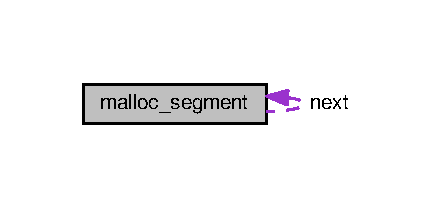
\includegraphics[width=208pt]{structmalloc__segment__coll__graph}
\end{center}
\end{figure}
\subsection*{Data Fields}
\begin{DoxyCompactItemize}
\item 
char $\ast$ {\bfseries base}\hypertarget{structmalloc__segment_ad4c68a4113c3a4f9b167aadaa7c31b89}{}\label{structmalloc__segment_ad4c68a4113c3a4f9b167aadaa7c31b89}

\item 
size\+\_\+t {\bfseries size}\hypertarget{structmalloc__segment_a392a23ee3bd7a167e5f6382793a8eba1}{}\label{structmalloc__segment_a392a23ee3bd7a167e5f6382793a8eba1}

\item 
struct \hyperlink{structmalloc__segment}{malloc\+\_\+segment} $\ast$ {\bfseries next}\hypertarget{structmalloc__segment_a92c4c9f618dba33fd8628d743cc02f5a}{}\label{structmalloc__segment_a92c4c9f618dba33fd8628d743cc02f5a}

\item 
flag\+\_\+t {\bfseries sflags}\hypertarget{structmalloc__segment_ac48f17d9495d732749db6544cabbec2c}{}\label{structmalloc__segment_ac48f17d9495d732749db6544cabbec2c}

\end{DoxyCompactItemize}


The documentation for this struct was generated from the following file\+:\begin{DoxyCompactItemize}
\item 
gprolog-\/utf8-\/tree/src/\+Engine\+Pl/dl\+\_\+malloc.\+c\end{DoxyCompactItemize}

\hypertarget{structmalloc__state}{}\section{malloc\+\_\+state Struct Reference}
\label{structmalloc__state}\index{malloc\+\_\+state@{malloc\+\_\+state}}


Collaboration diagram for malloc\+\_\+state\+:\nopagebreak
\begin{figure}[H]
\begin{center}
\leavevmode
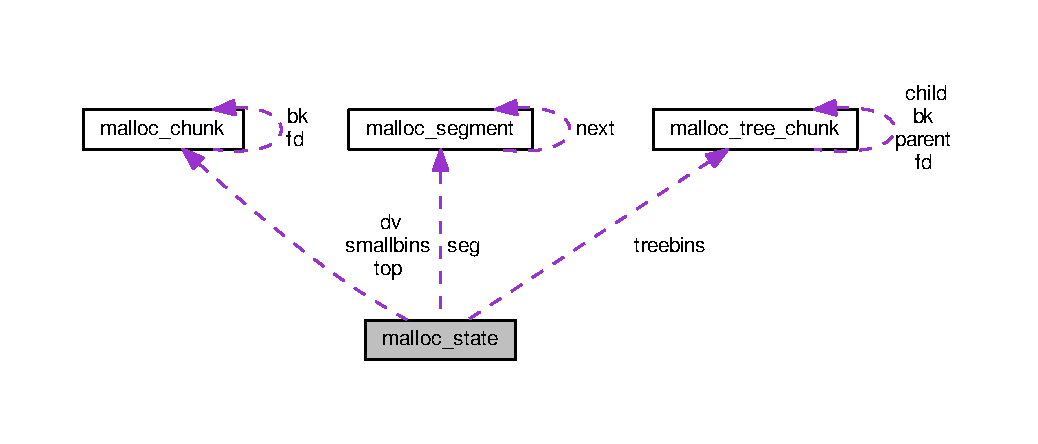
\includegraphics[width=350pt]{structmalloc__state__coll__graph}
\end{center}
\end{figure}
\subsection*{Data Fields}
\begin{DoxyCompactItemize}
\item 
binmap\+\_\+t {\bfseries smallmap}\hypertarget{structmalloc__state_a9e597125e4a96b39d3859c59fee38c49}{}\label{structmalloc__state_a9e597125e4a96b39d3859c59fee38c49}

\item 
binmap\+\_\+t {\bfseries treemap}\hypertarget{structmalloc__state_ae20bf1bcda1838e5bc07d2395ba72283}{}\label{structmalloc__state_ae20bf1bcda1838e5bc07d2395ba72283}

\item 
size\+\_\+t {\bfseries dvsize}\hypertarget{structmalloc__state_ae2e6a3ed8e8abaf03e47917057f1012d}{}\label{structmalloc__state_ae2e6a3ed8e8abaf03e47917057f1012d}

\item 
size\+\_\+t {\bfseries topsize}\hypertarget{structmalloc__state_aa93901fa8e414a7d7881ee968b097eea}{}\label{structmalloc__state_aa93901fa8e414a7d7881ee968b097eea}

\item 
char $\ast$ {\bfseries least\+\_\+addr}\hypertarget{structmalloc__state_af9a424730d25d685373ab736a29560b5}{}\label{structmalloc__state_af9a424730d25d685373ab736a29560b5}

\item 
\hyperlink{structmalloc__chunk}{mchunkptr} {\bfseries dv}\hypertarget{structmalloc__state_a840943ad4baaddbaaa5defe954ec06b9}{}\label{structmalloc__state_a840943ad4baaddbaaa5defe954ec06b9}

\item 
\hyperlink{structmalloc__chunk}{mchunkptr} {\bfseries top}\hypertarget{structmalloc__state_a594c4d03c189612e0ce91f7aba8dae77}{}\label{structmalloc__state_a594c4d03c189612e0ce91f7aba8dae77}

\item 
size\+\_\+t {\bfseries trim\+\_\+check}\hypertarget{structmalloc__state_a30209a5277132d0f207c7a850d225324}{}\label{structmalloc__state_a30209a5277132d0f207c7a850d225324}

\item 
size\+\_\+t {\bfseries release\+\_\+checks}\hypertarget{structmalloc__state_af2afbe4faf64185994d9c10cef2e0a3a}{}\label{structmalloc__state_af2afbe4faf64185994d9c10cef2e0a3a}

\item 
size\+\_\+t {\bfseries magic}\hypertarget{structmalloc__state_ac19e13bf018dc22419c38d8cbe839b62}{}\label{structmalloc__state_ac19e13bf018dc22419c38d8cbe839b62}

\item 
\hyperlink{structmalloc__chunk}{mchunkptr} {\bfseries smallbins} \mbox{[}(N\+S\+M\+A\+L\+L\+B\+I\+NS+1)$\ast$2\mbox{]}\hypertarget{structmalloc__state_ade50b83b94e4f09d372a18ae51c13f70}{}\label{structmalloc__state_ade50b83b94e4f09d372a18ae51c13f70}

\item 
\hyperlink{structmalloc__tree__chunk}{tbinptr} {\bfseries treebins} \mbox{[}N\+T\+R\+E\+E\+B\+I\+NS\mbox{]}\hypertarget{structmalloc__state_a7ccf88dffa5e3287b7c9dd290ea1a0cb}{}\label{structmalloc__state_a7ccf88dffa5e3287b7c9dd290ea1a0cb}

\item 
size\+\_\+t {\bfseries footprint}\hypertarget{structmalloc__state_a77ec93dc40bb85bd7a3c4e9b26547d11}{}\label{structmalloc__state_a77ec93dc40bb85bd7a3c4e9b26547d11}

\item 
size\+\_\+t {\bfseries max\+\_\+footprint}\hypertarget{structmalloc__state_ac5c720358079598dfb5d699124e761c8}{}\label{structmalloc__state_ac5c720358079598dfb5d699124e761c8}

\item 
size\+\_\+t {\bfseries footprint\+\_\+limit}\hypertarget{structmalloc__state_ab589c6129376d79aab99babfe55fe048}{}\label{structmalloc__state_ab589c6129376d79aab99babfe55fe048}

\item 
flag\+\_\+t {\bfseries mflags}\hypertarget{structmalloc__state_a44ff83ca07796cad96f2289471c88d2d}{}\label{structmalloc__state_a44ff83ca07796cad96f2289471c88d2d}

\item 
M\+L\+O\+C\+K\+\_\+T {\bfseries mutex}\hypertarget{structmalloc__state_aafbde3a2fbb7df9480eb14521e5624da}{}\label{structmalloc__state_aafbde3a2fbb7df9480eb14521e5624da}

\item 
\hyperlink{structmalloc__segment}{msegment} {\bfseries seg}\hypertarget{structmalloc__state_a899c69eca79f165b03913063a93d973a}{}\label{structmalloc__state_a899c69eca79f165b03913063a93d973a}

\item 
void $\ast$ {\bfseries extp}\hypertarget{structmalloc__state_aa605a719561fc44ce2ce7165e6dcb897}{}\label{structmalloc__state_aa605a719561fc44ce2ce7165e6dcb897}

\item 
size\+\_\+t {\bfseries exts}\hypertarget{structmalloc__state_af3c1e272f4107a5006ee10429cb2232a}{}\label{structmalloc__state_af3c1e272f4107a5006ee10429cb2232a}

\end{DoxyCompactItemize}


The documentation for this struct was generated from the following file\+:\begin{DoxyCompactItemize}
\item 
gprolog-\/utf8-\/tree/src/\+Engine\+Pl/dl\+\_\+malloc.\+c\end{DoxyCompactItemize}

\hypertarget{structmalloc__tree__chunk}{}\section{malloc\+\_\+tree\+\_\+chunk Struct Reference}
\label{structmalloc__tree__chunk}\index{malloc\+\_\+tree\+\_\+chunk@{malloc\+\_\+tree\+\_\+chunk}}


Collaboration diagram for malloc\+\_\+tree\+\_\+chunk\+:\nopagebreak
\begin{figure}[H]
\begin{center}
\leavevmode
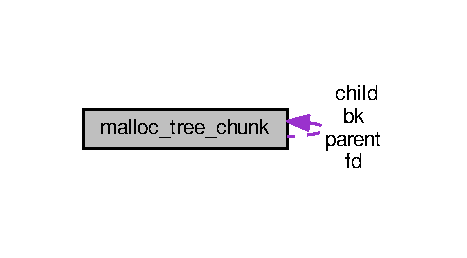
\includegraphics[width=224pt]{structmalloc__tree__chunk__coll__graph}
\end{center}
\end{figure}
\subsection*{Data Fields}
\begin{DoxyCompactItemize}
\item 
size\+\_\+t {\bfseries prev\+\_\+foot}\hypertarget{structmalloc__tree__chunk_a0b7e321702857b18f5013a3182b99262}{}\label{structmalloc__tree__chunk_a0b7e321702857b18f5013a3182b99262}

\item 
size\+\_\+t {\bfseries head}\hypertarget{structmalloc__tree__chunk_a1737b1a78f4bfbf0047210e3f3fd014d}{}\label{structmalloc__tree__chunk_a1737b1a78f4bfbf0047210e3f3fd014d}

\item 
struct \hyperlink{structmalloc__tree__chunk}{malloc\+\_\+tree\+\_\+chunk} $\ast$ {\bfseries fd}\hypertarget{structmalloc__tree__chunk_a5584ad2f70ef7ad1a5eb5f55820e3fe9}{}\label{structmalloc__tree__chunk_a5584ad2f70ef7ad1a5eb5f55820e3fe9}

\item 
struct \hyperlink{structmalloc__tree__chunk}{malloc\+\_\+tree\+\_\+chunk} $\ast$ {\bfseries bk}\hypertarget{structmalloc__tree__chunk_a862e6cafa961c1f63d4b10d67480cba0}{}\label{structmalloc__tree__chunk_a862e6cafa961c1f63d4b10d67480cba0}

\item 
struct \hyperlink{structmalloc__tree__chunk}{malloc\+\_\+tree\+\_\+chunk} $\ast$ {\bfseries child} \mbox{[}2\mbox{]}\hypertarget{structmalloc__tree__chunk_a560fa0afc644c1e05f4fab62818ab6cd}{}\label{structmalloc__tree__chunk_a560fa0afc644c1e05f4fab62818ab6cd}

\item 
struct \hyperlink{structmalloc__tree__chunk}{malloc\+\_\+tree\+\_\+chunk} $\ast$ {\bfseries parent}\hypertarget{structmalloc__tree__chunk_ae15ae9af5d9c57488718f0649868b7fe}{}\label{structmalloc__tree__chunk_ae15ae9af5d9c57488718f0649868b7fe}

\item 
bindex\+\_\+t {\bfseries index}\hypertarget{structmalloc__tree__chunk_a3015f2a8d6cc5cdb7abaf34e902c46a4}{}\label{structmalloc__tree__chunk_a3015f2a8d6cc5cdb7abaf34e902c46a4}

\end{DoxyCompactItemize}


The documentation for this struct was generated from the following file\+:\begin{DoxyCompactItemize}
\item 
gprolog-\/utf8-\/tree/src/\+Engine\+Pl/dl\+\_\+malloc.\+c\end{DoxyCompactItemize}

\hypertarget{structMem}{}\section{Mem Struct Reference}
\label{structMem}\index{Mem@{Mem}}


{\ttfamily \#include $<$ma\+\_\+parser.\+h$>$}

\subsection*{Data Fields}
\begin{DoxyCompactItemize}
\item 
char $\ast$ \hyperlink{structMem_a97d3d596dc096d506a21a183f733ef5d}{name}
\item 
int \hyperlink{structMem_a496c7609b4591655a4acf6113a892c2d}{index}
\end{DoxyCompactItemize}


\subsection{Field Documentation}
\index{Mem@{Mem}!index@{index}}
\index{index@{index}!Mem@{Mem}}
\subsubsection[{\texorpdfstring{index}{index}}]{\setlength{\rightskip}{0pt plus 5cm}int Mem\+::index}\hypertarget{structMem_a496c7609b4591655a4acf6113a892c2d}{}\label{structMem_a496c7609b4591655a4acf6113a892c2d}
\index{Mem@{Mem}!name@{name}}
\index{name@{name}!Mem@{Mem}}
\subsubsection[{\texorpdfstring{name}{name}}]{\setlength{\rightskip}{0pt plus 5cm}char$\ast$ Mem\+::name}\hypertarget{structMem_a97d3d596dc096d506a21a183f733ef5d}{}\label{structMem_a97d3d596dc096d506a21a183f733ef5d}


The documentation for this struct was generated from the following file\+:\begin{DoxyCompactItemize}
\item 
gprolog-\/utf8-\/tree/src/\+Ma2\+Asm/\hyperlink{ma__parser_8h}{ma\+\_\+parser.\+h}\end{DoxyCompactItemize}

\hypertarget{structMonom}{}\section{Monom Struct Reference}
\label{structMonom}\index{Monom@{Monom}}
\subsection*{Data Fields}
\begin{DoxyCompactItemize}
\item 
Pl\+Long {\bfseries a}\hypertarget{structMonom_a65b12a1274c4471fce35332ef4bb84f6}{}\label{structMonom_a65b12a1274c4471fce35332ef4bb84f6}

\item 
Wam\+Word {\bfseries x\+\_\+word}\hypertarget{structMonom_a72cc88b43a8727f47d9e50db2cda700f}{}\label{structMonom_a72cc88b43a8727f47d9e50db2cda700f}

\end{DoxyCompactItemize}


The documentation for this struct was generated from the following file\+:\begin{DoxyCompactItemize}
\item 
gprolog-\/utf8-\/tree/src/\+Bips\+F\+D/math\+\_\+supp.\+c\end{DoxyCompactItemize}

\hypertarget{structNonLin}{}\section{Non\+Lin Struct Reference}
\label{structNonLin}\index{Non\+Lin@{Non\+Lin}}
\subsection*{Data Fields}
\begin{DoxyCompactItemize}
\item 
int {\bfseries cstr}\hypertarget{structNonLin_ace702860218e3fed62bb3235547358aa}{}\label{structNonLin_ace702860218e3fed62bb3235547358aa}

\item 
Wam\+Word {\bfseries a1}\hypertarget{structNonLin_a143b9a64bce8684b7cc00bea2c48639b}{}\label{structNonLin_a143b9a64bce8684b7cc00bea2c48639b}

\item 
Wam\+Word {\bfseries a2}\hypertarget{structNonLin_a94219bccdea182e374720870a013da88}{}\label{structNonLin_a94219bccdea182e374720870a013da88}

\item 
Wam\+Word {\bfseries a3}\hypertarget{structNonLin_a3e4eeac9f54cd48366e50824833a9271}{}\label{structNonLin_a3e4eeac9f54cd48366e50824833a9271}

\item 
Wam\+Word {\bfseries res}\hypertarget{structNonLin_af8f4e398e6c9371309ae73d04456f4f0}{}\label{structNonLin_af8f4e398e6c9371309ae73d04456f4f0}

\end{DoxyCompactItemize}


The documentation for this struct was generated from the following file\+:\begin{DoxyCompactItemize}
\item 
gprolog-\/utf8-\/tree/src/\+Bips\+F\+D/math\+\_\+supp.\+c\end{DoxyCompactItemize}

\hypertarget{structObjInf}{}\section{Obj\+Inf Struct Reference}
\label{structObjInf}\index{Obj\+Inf@{Obj\+Inf}}
\subsection*{Data Fields}
\begin{DoxyCompactItemize}
\item 
void($\ast$ {\bfseries fct\+\_\+obj\+\_\+init} )()\hypertarget{structObjInf_a87ba4456d48d1ca4b94a0d0e7f44650c}{}\label{structObjInf_a87ba4456d48d1ca4b94a0d0e7f44650c}

\item 
void($\ast$ {\bfseries fct\+\_\+exec\+\_\+system} )()\hypertarget{structObjInf_a5b3f237a232e4cfae91c10bfe78f163f}{}\label{structObjInf_a5b3f237a232e4cfae91c10bfe78f163f}

\item 
void($\ast$ {\bfseries fct\+\_\+exec\+\_\+user} )()\hypertarget{structObjInf_a394489a76d14d4711797e459a15ebfb4}{}\label{structObjInf_a394489a76d14d4711797e459a15ebfb4}

\end{DoxyCompactItemize}


The documentation for this struct was generated from the following file\+:\begin{DoxyCompactItemize}
\item 
gprolog-\/utf8-\/tree/src/\+Engine\+Pl/obj\+\_\+chain.\+c\end{DoxyCompactItemize}

\hypertarget{structonesol}{}\section{onesol Struct Reference}
\label{structonesol}\index{onesol@{onesol}}


Collaboration diagram for onesol\+:\nopagebreak
\begin{figure}[H]
\begin{center}
\leavevmode
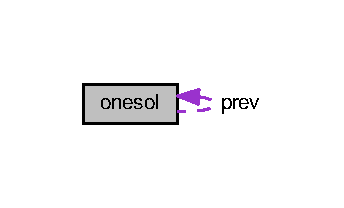
\includegraphics[width=165pt]{structonesol__coll__graph}
\end{center}
\end{figure}
\subsection*{Data Fields}
\begin{DoxyCompactItemize}
\item 
\hyperlink{structonesol}{One\+SolP} {\bfseries prev}\hypertarget{structonesol_a67474d69d62f74ecb1da52cf3a6fd255}{}\label{structonesol_a67474d69d62f74ecb1da52cf3a6fd255}

\item 
int {\bfseries sol\+\_\+no}\hypertarget{structonesol_adf8141bfb4d67ec7ef0cdb66abc2e03d}{}\label{structonesol_adf8141bfb4d67ec7ef0cdb66abc2e03d}

\item 
int {\bfseries term\+\_\+size}\hypertarget{structonesol_a7d00bc5747882c6030eff6839217f1d5}{}\label{structonesol_a7d00bc5747882c6030eff6839217f1d5}

\item 
Wam\+Word {\bfseries term\+\_\+word}\hypertarget{structonesol_ad2da50a130c4212644b22689ded445bf}{}\label{structonesol_ad2da50a130c4212644b22689ded445bf}

\end{DoxyCompactItemize}


The documentation for this struct was generated from the following file\+:\begin{DoxyCompactItemize}
\item 
gprolog-\/utf8-\/tree/src/\+Bips\+Pl/all\+\_\+solut\+\_\+c.\+c\end{DoxyCompactItemize}

\hypertarget{structOperInf}{}\section{Oper\+Inf Struct Reference}
\label{structOperInf}\index{Oper\+Inf@{Oper\+Inf}}


{\ttfamily \#include $<$oper.\+h$>$}

\subsection*{Data Fields}
\begin{DoxyCompactItemize}
\item 
\hyperlink{gprolog_8h_a4d005b136d7fb28537eb1815f7868b63}{Pl\+Long} \hyperlink{structOperInf_a5ab08736fa238d100509038e938fe187}{a\+\_\+t}
\item 
int \hyperlink{structOperInf_a50a4ec676df2b3555058f59753d48698}{prec}
\item 
int \hyperlink{structOperInf_afbf02377f941f53f5cd63f151c2da1f0}{left}
\item 
int \hyperlink{structOperInf_a558dc457885d6b96f6d8f833f1ce6c66}{right}
\end{DoxyCompactItemize}


\subsection{Field Documentation}
\index{Oper\+Inf@{Oper\+Inf}!a\+\_\+t@{a\+\_\+t}}
\index{a\+\_\+t@{a\+\_\+t}!Oper\+Inf@{Oper\+Inf}}
\subsubsection[{\texorpdfstring{a\+\_\+t}{a_t}}]{\setlength{\rightskip}{0pt plus 5cm}{\bf Pl\+Long} Oper\+Inf\+::a\+\_\+t}\hypertarget{structOperInf_a5ab08736fa238d100509038e938fe187}{}\label{structOperInf_a5ab08736fa238d100509038e938fe187}
\index{Oper\+Inf@{Oper\+Inf}!left@{left}}
\index{left@{left}!Oper\+Inf@{Oper\+Inf}}
\subsubsection[{\texorpdfstring{left}{left}}]{\setlength{\rightskip}{0pt plus 5cm}int Oper\+Inf\+::left}\hypertarget{structOperInf_afbf02377f941f53f5cd63f151c2da1f0}{}\label{structOperInf_afbf02377f941f53f5cd63f151c2da1f0}
\index{Oper\+Inf@{Oper\+Inf}!prec@{prec}}
\index{prec@{prec}!Oper\+Inf@{Oper\+Inf}}
\subsubsection[{\texorpdfstring{prec}{prec}}]{\setlength{\rightskip}{0pt plus 5cm}int Oper\+Inf\+::prec}\hypertarget{structOperInf_a50a4ec676df2b3555058f59753d48698}{}\label{structOperInf_a50a4ec676df2b3555058f59753d48698}
\index{Oper\+Inf@{Oper\+Inf}!right@{right}}
\index{right@{right}!Oper\+Inf@{Oper\+Inf}}
\subsubsection[{\texorpdfstring{right}{right}}]{\setlength{\rightskip}{0pt plus 5cm}int Oper\+Inf\+::right}\hypertarget{structOperInf_a558dc457885d6b96f6d8f833f1ce6c66}{}\label{structOperInf_a558dc457885d6b96f6d8f833f1ce6c66}


The documentation for this struct was generated from the following file\+:\begin{DoxyCompactItemize}
\item 
gprolog-\/utf8-\/tree/src/\+Engine\+Pl/\hyperlink{oper_8h}{oper.\+h}\end{DoxyCompactItemize}

\hypertarget{structParseInf}{}\section{Parse\+Inf Struct Reference}
\label{structParseInf}\index{Parse\+Inf@{Parse\+Inf}}
\subsection*{Data Fields}
\begin{DoxyCompactItemize}
\item 
char $\ast$ {\bfseries keyword}\hypertarget{structParseInf_affadb424830268d2231588e867b1fb40}{}\label{structParseInf_affadb424830268d2231588e867b1fb40}

\item 
void($\ast$ {\bfseries fct} )()\hypertarget{structParseInf_a17e09c905211b8d0ac00827aeeea9237}{}\label{structParseInf_a17e09c905211b8d0ac00827aeeea9237}

\item 
int {\bfseries nb\+\_\+args}\hypertarget{structParseInf_abb84b55b8b29fe0bccf151d7400f0d9d}{}\label{structParseInf_abb84b55b8b29fe0bccf151d7400f0d9d}

\item 
Arg\+Typ {\bfseries arg\+\_\+type} \mbox{[}M\+A\+X\+\_\+\+F\+C\+T\+\_\+\+A\+R\+I\+TY\mbox{]}\hypertarget{structParseInf_a4bc1d3c3237113de20adb4050419bca6}{}\label{structParseInf_a4bc1d3c3237113de20adb4050419bca6}

\end{DoxyCompactItemize}


The documentation for this struct was generated from the following file\+:\begin{DoxyCompactItemize}
\item 
gprolog-\/utf8-\/tree/src/\+Wam2\+Ma/wam\+\_\+parser.\+c\end{DoxyCompactItemize}

\hypertarget{structPbStk}{}\section{Pb\+Stk Struct Reference}
\label{structPbStk}\index{Pb\+Stk@{Pb\+Stk}}


{\ttfamily \#include $<$stream\+\_\+supp.\+h$>$}

\subsection*{Data Fields}
\begin{DoxyCompactItemize}
\item 
int \hyperlink{structPbStk_a753c451400807eac788034c15a4e9810}{buff} \mbox{[}\hyperlink{stream__supp_8h_a7c01809509d811cfc0c70e47443a9613}{S\+T\+R\+E\+A\+M\+\_\+\+P\+B\+\_\+\+S\+I\+ZE}\mbox{]}
\item 
int $\ast$ \hyperlink{structPbStk_a739af7eef937b961dc73fec61672bee2}{ptr}
\item 
int \hyperlink{structPbStk_a222a0c77b4b0feef1323dc7cf1f0e74b}{nb\+\_\+elems}
\end{DoxyCompactItemize}


\subsection{Field Documentation}
\index{Pb\+Stk@{Pb\+Stk}!buff@{buff}}
\index{buff@{buff}!Pb\+Stk@{Pb\+Stk}}
\subsubsection[{\texorpdfstring{buff}{buff}}]{\setlength{\rightskip}{0pt plus 5cm}int Pb\+Stk\+::buff\mbox{[}{\bf S\+T\+R\+E\+A\+M\+\_\+\+P\+B\+\_\+\+S\+I\+ZE}\mbox{]}}\hypertarget{structPbStk_a753c451400807eac788034c15a4e9810}{}\label{structPbStk_a753c451400807eac788034c15a4e9810}
\index{Pb\+Stk@{Pb\+Stk}!nb\+\_\+elems@{nb\+\_\+elems}}
\index{nb\+\_\+elems@{nb\+\_\+elems}!Pb\+Stk@{Pb\+Stk}}
\subsubsection[{\texorpdfstring{nb\+\_\+elems}{nb_elems}}]{\setlength{\rightskip}{0pt plus 5cm}int Pb\+Stk\+::nb\+\_\+elems}\hypertarget{structPbStk_a222a0c77b4b0feef1323dc7cf1f0e74b}{}\label{structPbStk_a222a0c77b4b0feef1323dc7cf1f0e74b}
\index{Pb\+Stk@{Pb\+Stk}!ptr@{ptr}}
\index{ptr@{ptr}!Pb\+Stk@{Pb\+Stk}}
\subsubsection[{\texorpdfstring{ptr}{ptr}}]{\setlength{\rightskip}{0pt plus 5cm}int$\ast$ Pb\+Stk\+::ptr}\hypertarget{structPbStk_a739af7eef937b961dc73fec61672bee2}{}\label{structPbStk_a739af7eef937b961dc73fec61672bee2}


The documentation for this struct was generated from the following file\+:\begin{DoxyCompactItemize}
\item 
gprolog-\/utf8-\/tree/src/\+Bips\+Pl/\hyperlink{stream__supp_8h}{stream\+\_\+supp.\+h}\end{DoxyCompactItemize}

\hypertarget{structPlFIOArg}{}\section{Pl\+F\+I\+O\+Arg Struct Reference}
\label{structPlFIOArg}\index{Pl\+F\+I\+O\+Arg@{Pl\+F\+I\+O\+Arg}}
\subsection*{Data Fields}
\begin{DoxyCompactItemize}
\item 
Bool {\bfseries is\+\_\+var}\hypertarget{structPlFIOArg_ad700005317887006bd276a4d1a177881}{}\label{structPlFIOArg_ad700005317887006bd276a4d1a177881}

\item 
Bool {\bfseries unify}\hypertarget{structPlFIOArg_a6394f30ef4d8a74b9a1e731a9f725a35}{}\label{structPlFIOArg_a6394f30ef4d8a74b9a1e731a9f725a35}

\item 
\begin{tabbing}
xx\=xx\=xx\=xx\=xx\=xx\=xx\=xx\=xx\=\kill
union \{\\
\>PlLong {\bfseries l}\\
\>char $\ast$ {\bfseries s}\\
\>double {\bfseries d}\\
\} {\bfseries value}\hypertarget{structPlFIOArg_a69180a58f761dcda790af38c4c0ca5a2}{}\label{structPlFIOArg_a69180a58f761dcda790af38c4c0ca5a2}
\\

\end{tabbing}\item 
Pl\+Bool {\bfseries is\+\_\+var}\hypertarget{structPlFIOArg_ab4d9b51a4575a50e1d9b8a3ec36a3f6e}{}\label{structPlFIOArg_ab4d9b51a4575a50e1d9b8a3ec36a3f6e}

\item 
Pl\+Bool {\bfseries unify}\hypertarget{structPlFIOArg_a3d5c4af7de4d733aa3806b29081336b8}{}\label{structPlFIOArg_a3d5c4af7de4d733aa3806b29081336b8}

\item 
\begin{tabbing}
xx\=xx\=xx\=xx\=xx\=xx\=xx\=xx\=xx\=\kill
union \{\\
\>PlLong {\bfseries l}\\
\>char $\ast$ {\bfseries s}\\
\>double {\bfseries d}\\
\} {\bfseries value}\hypertarget{structPlFIOArg_a1588d26dbc95302b6b7a0b79715ead8e}{}\label{structPlFIOArg_a1588d26dbc95302b6b7a0b79715ead8e}
\\

\end{tabbing}\end{DoxyCompactItemize}


The documentation for this struct was generated from the following files\+:\begin{DoxyCompactItemize}
\item 
gprolog-\/utf8-\/tree/src/\+Bips\+Pl/foreign\+\_\+supp.\+h\item 
gprolog-\/utf8-\/tree/src/\+Engine\+Pl/gprolog.\+h\end{DoxyCompactItemize}

\hypertarget{structPoly}{}\section{Poly Struct Reference}
\label{structPoly}\index{Poly@{Poly}}


Collaboration diagram for Poly\+:\nopagebreak
\begin{figure}[H]
\begin{center}
\leavevmode
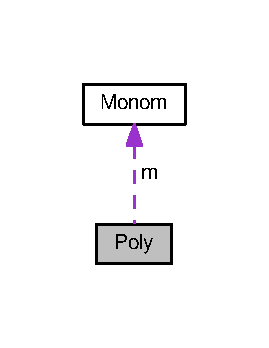
\includegraphics[width=129pt]{structPoly__coll__graph}
\end{center}
\end{figure}
\subsection*{Data Fields}
\begin{DoxyCompactItemize}
\item 
Pl\+Long {\bfseries c}\hypertarget{structPoly_ac87064f885d4389f545b4194de01f60e}{}\label{structPoly_ac87064f885d4389f545b4194de01f60e}

\item 
int {\bfseries nb\+\_\+monom}\hypertarget{structPoly_a23949f807fc70dcf7c1b7b18bb48be0c}{}\label{structPoly_a23949f807fc70dcf7c1b7b18bb48be0c}

\item 
\hyperlink{structMonom}{Monom} {\bfseries m} \mbox{[}M\+A\+X\+\_\+\+M\+O\+N\+O\+MS\mbox{]}\hypertarget{structPoly_a1bae103a920d8182006ef10891c87906}{}\label{structPoly_a1bae103a920d8182006ef10891c87906}

\end{DoxyCompactItemize}


The documentation for this struct was generated from the following file\+:\begin{DoxyCompactItemize}
\item 
gprolog-\/utf8-\/tree/src/\+Bips\+F\+D/math\+\_\+supp.\+c\end{DoxyCompactItemize}

\hypertarget{structpredinf}{}\section{predinf Struct Reference}
\label{structpredinf}\index{predinf@{predinf}}


Collaboration diagram for predinf\+:\nopagebreak
\begin{figure}[H]
\begin{center}
\leavevmode
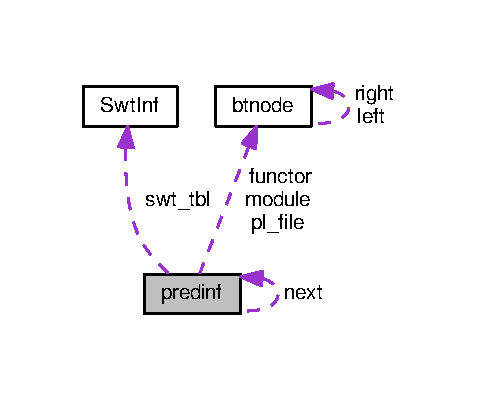
\includegraphics[width=230pt]{structpredinf__coll__graph}
\end{center}
\end{figure}
\subsection*{Data Fields}
\begin{DoxyCompactItemize}
\item 
\hyperlink{structbtnode}{B\+T\+Node} $\ast$ {\bfseries module}\hypertarget{structpredinf_a5f44f90f1226e1463e76665aaf490a9d}{}\label{structpredinf_a5f44f90f1226e1463e76665aaf490a9d}

\item 
\hyperlink{structbtnode}{B\+T\+Node} $\ast$ {\bfseries functor}\hypertarget{structpredinf_a6ae4c5cbb30b0db0b0dde51084453eee}{}\label{structpredinf_a6ae4c5cbb30b0db0b0dde51084453eee}

\item 
int {\bfseries arity}\hypertarget{structpredinf_a16871c2b0c2e29058abe513301f0b7b0}{}\label{structpredinf_a16871c2b0c2e29058abe513301f0b7b0}

\item 
char $\ast$ {\bfseries hexa}\hypertarget{structpredinf_ab6fc21ba8f80aea382dfd11b9a50e7ac}{}\label{structpredinf_ab6fc21ba8f80aea382dfd11b9a50e7ac}

\item 
int {\bfseries line\+\_\+no}\hypertarget{structpredinf_ae858dcfb66886799f41d0042ccf8667e}{}\label{structpredinf_ae858dcfb66886799f41d0042ccf8667e}

\item 
int {\bfseries prop}\hypertarget{structpredinf_a39785936db83e7bcf5036b5365423c5e}{}\label{structpredinf_a39785936db83e7bcf5036b5365423c5e}

\item 
\hyperlink{structbtnode}{B\+T\+Node} $\ast$ {\bfseries pl\+\_\+file}\hypertarget{structpredinf_a85bb945f5415fd2177b55ce91562c36c}{}\label{structpredinf_a85bb945f5415fd2177b55ce91562c36c}

\item 
int {\bfseries pl\+\_\+line}\hypertarget{structpredinf_a0bb58f984add8b6a8e040181a8181cbd}{}\label{structpredinf_a0bb58f984add8b6a8e040181a8181cbd}

\item 
\hyperlink{structSwtInf}{Swt\+Tbl} $\ast$ {\bfseries swt\+\_\+tbl} \mbox{[}3\mbox{]}\hypertarget{structpredinf_a9e448a6b5c08b225ac0a07043f3a37c9}{}\label{structpredinf_a9e448a6b5c08b225ac0a07043f3a37c9}

\item 
\hyperlink{structpredinf}{PredP} {\bfseries next}\hypertarget{structpredinf_a5640b4a5b40d6208119e14349a52d8db}{}\label{structpredinf_a5640b4a5b40d6208119e14349a52d8db}

\end{DoxyCompactItemize}


The documentation for this struct was generated from the following file\+:\begin{DoxyCompactItemize}
\item 
gprolog-\/utf8-\/tree/src/\+Wam2\+Ma/wam2ma.\+c\end{DoxyCompactItemize}

\hypertarget{structPredInf}{}\section{Pred\+Inf Struct Reference}
\label{structPredInf}\index{Pred\+Inf@{Pred\+Inf}}
\subsection*{Data Fields}
\begin{DoxyCompactItemize}
\item 
Pl\+Long {\bfseries f\+\_\+n}\hypertarget{structPredInf_ac0b2b557f702cda0d5111bc65630d5a3}{}\label{structPredInf_ac0b2b557f702cda0d5111bc65630d5a3}

\item 
int {\bfseries pl\+\_\+file}\hypertarget{structPredInf_a0d5ac69f7fce6062b3327fc2badc1658}{}\label{structPredInf_a0d5ac69f7fce6062b3327fc2badc1658}

\item 
int {\bfseries pl\+\_\+line}\hypertarget{structPredInf_a206ac901da36832f6111a542a2b8b11b}{}\label{structPredInf_a206ac901da36832f6111a542a2b8b11b}

\item 
int {\bfseries prop}\hypertarget{structPredInf_a2f0d287390fe634467a62f42f816d855}{}\label{structPredInf_a2f0d287390fe634467a62f42f816d855}

\item 
Pl\+Long $\ast$ {\bfseries codep}\hypertarget{structPredInf_a670788fe731440a8d7224e2729836dac}{}\label{structPredInf_a670788fe731440a8d7224e2729836dac}

\item 
Pl\+Long $\ast$ {\bfseries dyn}\hypertarget{structPredInf_aad15bc35f98eabb92f4ac4b9a35f65c0}{}\label{structPredInf_aad15bc35f98eabb92f4ac4b9a35f65c0}

\end{DoxyCompactItemize}


The documentation for this struct was generated from the following file\+:\begin{DoxyCompactItemize}
\item 
gprolog-\/utf8-\/tree/src/\+Engine\+Pl/pred.\+h\end{DoxyCompactItemize}

\hypertarget{structRange}{}\section{Range Struct Reference}
\label{structRange}\index{Range@{Range}}


{\ttfamily \#include $<$fd\+\_\+range.\+h$>$}

\subsection*{Data Fields}
\begin{DoxyCompactItemize}
\item 
\hyperlink{bool_8h_afdcfe6db5bea87bd493a3fe2c513d5ef}{Bool} \hyperlink{structRange_a875104bdfb7f25377692ee3511b6cda7}{extra\+\_\+cstr}
\item 
int \hyperlink{structRange_ac3ccecdd1d8e143102bb4c2b5c0837d7}{min}
\item 
int \hyperlink{structRange_a7f490d5301f027e9defc4abf3970bf00}{max}
\item 
\hyperlink{fd__range_8h_a3cb8772380a4656f7d8c5d5c6346985e}{Vector} \hyperlink{structRange_aa1fc33857cb97860b7c55a8f90ad6e3f}{vec}
\end{DoxyCompactItemize}


\subsection{Field Documentation}
\index{Range@{Range}!extra\+\_\+cstr@{extra\+\_\+cstr}}
\index{extra\+\_\+cstr@{extra\+\_\+cstr}!Range@{Range}}
\subsubsection[{\texorpdfstring{extra\+\_\+cstr}{extra_cstr}}]{\setlength{\rightskip}{0pt plus 5cm}{\bf Bool} Range\+::extra\+\_\+cstr}\hypertarget{structRange_a875104bdfb7f25377692ee3511b6cda7}{}\label{structRange_a875104bdfb7f25377692ee3511b6cda7}
\index{Range@{Range}!max@{max}}
\index{max@{max}!Range@{Range}}
\subsubsection[{\texorpdfstring{max}{max}}]{\setlength{\rightskip}{0pt plus 5cm}int Range\+::max}\hypertarget{structRange_a7f490d5301f027e9defc4abf3970bf00}{}\label{structRange_a7f490d5301f027e9defc4abf3970bf00}
\index{Range@{Range}!min@{min}}
\index{min@{min}!Range@{Range}}
\subsubsection[{\texorpdfstring{min}{min}}]{\setlength{\rightskip}{0pt plus 5cm}int Range\+::min}\hypertarget{structRange_ac3ccecdd1d8e143102bb4c2b5c0837d7}{}\label{structRange_ac3ccecdd1d8e143102bb4c2b5c0837d7}
\index{Range@{Range}!vec@{vec}}
\index{vec@{vec}!Range@{Range}}
\subsubsection[{\texorpdfstring{vec}{vec}}]{\setlength{\rightskip}{0pt plus 5cm}{\bf Vector} Range\+::vec}\hypertarget{structRange_aa1fc33857cb97860b7c55a8f90ad6e3f}{}\label{structRange_aa1fc33857cb97860b7c55a8f90ad6e3f}


The documentation for this struct was generated from the following file\+:\begin{DoxyCompactItemize}
\item 
gprolog-\/utf8-\/tree/src/\+Engine\+F\+D/\hyperlink{fd__range_8h}{fd\+\_\+range.\+h}\end{DoxyCompactItemize}

\hypertarget{structRegInf}{}\section{Reg\+Inf Struct Reference}
\label{structRegInf}\index{Reg\+Inf@{Reg\+Inf}}
\subsection*{Data Fields}
\begin{DoxyCompactItemize}
\item 
char {\bfseries type} \mbox{[}32\mbox{]}\hypertarget{structRegInf_ac0222d4bcdce57bdcd74c2d45b9dfeb5}{}\label{structRegInf_ac0222d4bcdce57bdcd74c2d45b9dfeb5}

\item 
char {\bfseries name} \mbox{[}32\mbox{]}\hypertarget{structRegInf_af767d5a12d9d8e248f6c3eae99802e73}{}\label{structRegInf_af767d5a12d9d8e248f6c3eae99802e73}

\end{DoxyCompactItemize}


The documentation for this struct was generated from the following file\+:\begin{DoxyCompactItemize}
\item 
gprolog-\/utf8-\/tree/src/\+Engine\+Pl/pl\+\_\+config.\+c\end{DoxyCompactItemize}

\hypertarget{structSFOp}{}\section{S\+F\+Op Struct Reference}
\label{structSFOp}\index{S\+F\+Op@{S\+F\+Op}}
\subsection*{Data Fields}
\begin{DoxyCompactItemize}
\item 
int {\bfseries type}\hypertarget{structSFOp_a2edfc96ff91474523b5bda2185158ffa}{}\label{structSFOp_a2edfc96ff91474523b5bda2185158ffa}

\item 
int {\bfseries prec}\hypertarget{structSFOp_ae4c13ff3ed16b56c55f822e84b9db21a}{}\label{structSFOp_ae4c13ff3ed16b56c55f822e84b9db21a}

\item 
int {\bfseries left}\hypertarget{structSFOp_adc97e181b0efdcff6b921b82979ab80f}{}\label{structSFOp_adc97e181b0efdcff6b921b82979ab80f}

\item 
int {\bfseries right}\hypertarget{structSFOp_a53d1624dfd48f82123f055f8578646e7}{}\label{structSFOp_a53d1624dfd48f82123f055f8578646e7}

\item 
int {\bfseries length}\hypertarget{structSFOp_a3b91d02ed1a1a1c664a3cfb062e60ed1}{}\label{structSFOp_a3b91d02ed1a1a1c664a3cfb062e60ed1}

\end{DoxyCompactItemize}


The documentation for this struct was generated from the following file\+:\begin{DoxyCompactItemize}
\item 
gprolog-\/utf8-\/tree/src/\+Bips\+Pl/flag\+\_\+c.\+c\end{DoxyCompactItemize}

\hypertarget{structsr__file}{}\section{sr\+\_\+file Struct Reference}
\label{structsr__file}\index{sr\+\_\+file@{sr\+\_\+file}}


Collaboration diagram for sr\+\_\+file\+:\nopagebreak
\begin{figure}[H]
\begin{center}
\leavevmode
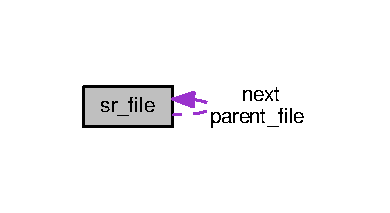
\includegraphics[width=187pt]{structsr__file__coll__graph}
\end{center}
\end{figure}
\subsection*{Data Fields}
\begin{DoxyCompactItemize}
\item 
int {\bfseries atom\+\_\+file\+\_\+name}\hypertarget{structsr__file_ae27edb1456ddb3b0453eca14e614c66b}{}\label{structsr__file_ae27edb1456ddb3b0453eca14e614c66b}

\item 
int {\bfseries stm}\hypertarget{structsr__file_a586a54828b5daba157cc712806a6f2b3}{}\label{structsr__file_a586a54828b5daba157cc712806a6f2b3}

\item 
Bool {\bfseries reposition}\hypertarget{structsr__file_a090b36b9b75dfbccd963f6787fd3f18e}{}\label{structsr__file_a090b36b9b75dfbccd963f6787fd3f18e}

\item 
char $\ast$ {\bfseries tmp\+\_\+path}\hypertarget{structsr__file_adc9ad8d65ba5f5b3bfc7a6c6ca329d88}{}\label{structsr__file_adc9ad8d65ba5f5b3bfc7a6c6ca329d88}

\item 
int {\bfseries tmp\+\_\+stm}\hypertarget{structsr__file_a200078e5cefb8ff2bd556997ff08b429}{}\label{structsr__file_a200078e5cefb8ff2bd556997ff08b429}

\item 
\hyperlink{structsr__file}{P\+S\+R\+File} {\bfseries next}\hypertarget{structsr__file_aa8623a318506eaad8a03faca16a7e72e}{}\label{structsr__file_aa8623a318506eaad8a03faca16a7e72e}

\item 
Bool {\bfseries eof\+\_\+reached}\hypertarget{structsr__file_ae76a89a158199f98536900d0fccdd0c4}{}\label{structsr__file_ae76a89a158199f98536900d0fccdd0c4}

\item 
int {\bfseries include\+\_\+line}\hypertarget{structsr__file_ae50c7011dac81b055f3cfbf64ae03598}{}\label{structsr__file_ae50c7011dac81b055f3cfbf64ae03598}

\item 
\hyperlink{structsr__file}{P\+S\+R\+File} {\bfseries parent\+\_\+file}\hypertarget{structsr__file_a57283a9f804b73dcd5bca6982ba8ac95}{}\label{structsr__file_a57283a9f804b73dcd5bca6982ba8ac95}

\end{DoxyCompactItemize}


The documentation for this struct was generated from the following file\+:\begin{DoxyCompactItemize}
\item 
gprolog-\/utf8-\/tree/src/\+Bips\+Pl/src\+\_\+rdr\+\_\+c.\+c\end{DoxyCompactItemize}

\hypertarget{structsr__module}{}\section{sr\+\_\+module Struct Reference}
\label{structsr__module}\index{sr\+\_\+module@{sr\+\_\+module}}


Collaboration diagram for sr\+\_\+module\+:\nopagebreak
\begin{figure}[H]
\begin{center}
\leavevmode
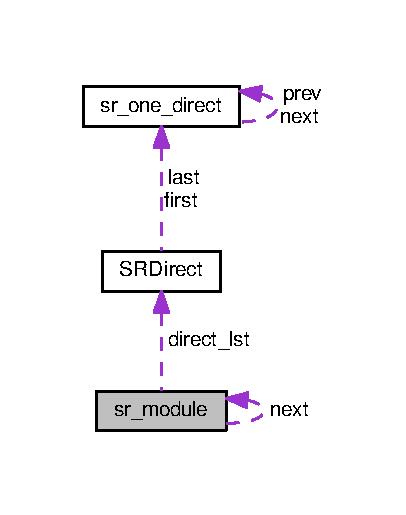
\includegraphics[width=195pt]{structsr__module__coll__graph}
\end{center}
\end{figure}
\subsection*{Data Fields}
\begin{DoxyCompactItemize}
\item 
int {\bfseries atom\+\_\+module\+\_\+name}\hypertarget{structsr__module_a5a1f181c93f13928623ca1426439eac8}{}\label{structsr__module_a5a1f181c93f13928623ca1426439eac8}

\item 
int {\bfseries i\+\_\+atom\+\_\+file\+\_\+def}\hypertarget{structsr__module_a2c69e68be4245afea2ed7d5a69650166}{}\label{structsr__module_a2c69e68be4245afea2ed7d5a69650166}

\item 
int {\bfseries i\+\_\+line\+\_\+def}\hypertarget{structsr__module_a931a2655c0576f16e2776c5c7ac2cf0a}{}\label{structsr__module_a931a2655c0576f16e2776c5c7ac2cf0a}

\item 
int {\bfseries b\+\_\+atom\+\_\+file\+\_\+def}\hypertarget{structsr__module_acc4948aadab6f3f5ae47ee8ea8c083ee}{}\label{structsr__module_acc4948aadab6f3f5ae47ee8ea8c083ee}

\item 
int {\bfseries b\+\_\+line\+\_\+def}\hypertarget{structsr__module_a0c96bc2505a798a709775e61787a1a24}{}\label{structsr__module_a0c96bc2505a798a709775e61787a1a24}

\item 
\hyperlink{structSRDirect}{S\+R\+Direct} {\bfseries direct\+\_\+lst}\hypertarget{structsr__module_a45a2eaca81407f38373afb940bb6dc57}{}\label{structsr__module_a45a2eaca81407f38373afb940bb6dc57}

\item 
\hyperlink{structsr__module}{P\+S\+R\+Module} {\bfseries next}\hypertarget{structsr__module_af8c9ce6870c7f7558096b050d6df683b}{}\label{structsr__module_af8c9ce6870c7f7558096b050d6df683b}

\end{DoxyCompactItemize}


The documentation for this struct was generated from the following file\+:\begin{DoxyCompactItemize}
\item 
gprolog-\/utf8-\/tree/src/\+Bips\+Pl/src\+\_\+rdr\+\_\+c.\+c\end{DoxyCompactItemize}

\hypertarget{structsr__one__direct}{}\section{sr\+\_\+one\+\_\+direct Struct Reference}
\label{structsr__one__direct}\index{sr\+\_\+one\+\_\+direct@{sr\+\_\+one\+\_\+direct}}


Collaboration diagram for sr\+\_\+one\+\_\+direct\+:\nopagebreak
\begin{figure}[H]
\begin{center}
\leavevmode
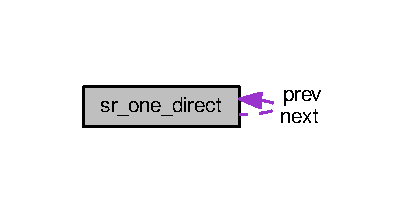
\includegraphics[width=195pt]{structsr__one__direct__coll__graph}
\end{center}
\end{figure}
\subsection*{Data Fields}
\begin{DoxyCompactItemize}
\item 
\hyperlink{src__rdr__c_8c_a03d2b46a29dc63fb6b0a6ec9378f36af}{S\+R\+Dir\+Type} \hyperlink{structsr__one__direct_ac59da886bfa2db8f18de3506965397f7}{type}
\item 
\hyperlink{LINUX__SIGSEGV_8c_a10ea8be8823feb38875b8a9326cbb424}{Wam\+Word} \hyperlink{structsr__one__direct_abe60646d574e029facc37a9b2491a74b}{a} \mbox{[}2\mbox{]}\mbox{[}3\mbox{]}
\item 
\hyperlink{src__rdr__c_8c_ad9901c46d3661cb327d1a08a1131e06a}{P\+S\+R\+One\+Direct} \hyperlink{structsr__one__direct_a601890e68d977d3467e52ab3a7ce9703}{next}
\item 
\hyperlink{src__rdr__c_8c_ad9901c46d3661cb327d1a08a1131e06a}{P\+S\+R\+One\+Direct} \hyperlink{structsr__one__direct_a25fd2e3df4af8e0f8cb89af0a1ea77f9}{prev}
\end{DoxyCompactItemize}


\subsection{Field Documentation}
\index{sr\+\_\+one\+\_\+direct@{sr\+\_\+one\+\_\+direct}!a@{a}}
\index{a@{a}!sr\+\_\+one\+\_\+direct@{sr\+\_\+one\+\_\+direct}}
\subsubsection[{\texorpdfstring{a}{a}}]{\setlength{\rightskip}{0pt plus 5cm}{\bf Wam\+Word} sr\+\_\+one\+\_\+direct\+::a\mbox{[}2\mbox{]}\mbox{[}3\mbox{]}}\hypertarget{structsr__one__direct_abe60646d574e029facc37a9b2491a74b}{}\label{structsr__one__direct_abe60646d574e029facc37a9b2491a74b}
\index{sr\+\_\+one\+\_\+direct@{sr\+\_\+one\+\_\+direct}!next@{next}}
\index{next@{next}!sr\+\_\+one\+\_\+direct@{sr\+\_\+one\+\_\+direct}}
\subsubsection[{\texorpdfstring{next}{next}}]{\setlength{\rightskip}{0pt plus 5cm}{\bf P\+S\+R\+One\+Direct} sr\+\_\+one\+\_\+direct\+::next}\hypertarget{structsr__one__direct_a601890e68d977d3467e52ab3a7ce9703}{}\label{structsr__one__direct_a601890e68d977d3467e52ab3a7ce9703}
\index{sr\+\_\+one\+\_\+direct@{sr\+\_\+one\+\_\+direct}!prev@{prev}}
\index{prev@{prev}!sr\+\_\+one\+\_\+direct@{sr\+\_\+one\+\_\+direct}}
\subsubsection[{\texorpdfstring{prev}{prev}}]{\setlength{\rightskip}{0pt plus 5cm}{\bf P\+S\+R\+One\+Direct} sr\+\_\+one\+\_\+direct\+::prev}\hypertarget{structsr__one__direct_a25fd2e3df4af8e0f8cb89af0a1ea77f9}{}\label{structsr__one__direct_a25fd2e3df4af8e0f8cb89af0a1ea77f9}
\index{sr\+\_\+one\+\_\+direct@{sr\+\_\+one\+\_\+direct}!type@{type}}
\index{type@{type}!sr\+\_\+one\+\_\+direct@{sr\+\_\+one\+\_\+direct}}
\subsubsection[{\texorpdfstring{type}{type}}]{\setlength{\rightskip}{0pt plus 5cm}{\bf S\+R\+Dir\+Type} sr\+\_\+one\+\_\+direct\+::type}\hypertarget{structsr__one__direct_ac59da886bfa2db8f18de3506965397f7}{}\label{structsr__one__direct_ac59da886bfa2db8f18de3506965397f7}


The documentation for this struct was generated from the following file\+:\begin{DoxyCompactItemize}
\item 
gprolog-\/utf8-\/tree/src/\+Bips\+Pl/\hyperlink{src__rdr__c_8c}{src\+\_\+rdr\+\_\+c.\+c}\end{DoxyCompactItemize}

\hypertarget{structSRDirect}{}\section{S\+R\+Direct Struct Reference}
\label{structSRDirect}\index{S\+R\+Direct@{S\+R\+Direct}}


Collaboration diagram for S\+R\+Direct\+:\nopagebreak
\begin{figure}[H]
\begin{center}
\leavevmode
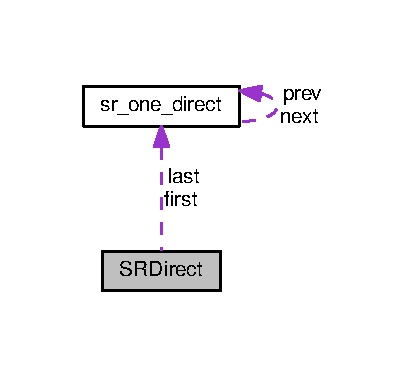
\includegraphics[width=195pt]{structSRDirect__coll__graph}
\end{center}
\end{figure}
\subsection*{Data Fields}
\begin{DoxyCompactItemize}
\item 
\hyperlink{src__rdr__c_8c_a901df9436a40f2eb43741da55a6dfd69}{S\+R\+One\+Direct} $\ast$ \hyperlink{structSRDirect_a418d898d49d9bfd256935f4e28bbf11b}{first}
\item 
\hyperlink{src__rdr__c_8c_a901df9436a40f2eb43741da55a6dfd69}{S\+R\+One\+Direct} $\ast$ \hyperlink{structSRDirect_aadd740950d79ebfff5baee79c33ced18}{last}
\end{DoxyCompactItemize}


\subsection{Field Documentation}
\index{S\+R\+Direct@{S\+R\+Direct}!first@{first}}
\index{first@{first}!S\+R\+Direct@{S\+R\+Direct}}
\subsubsection[{\texorpdfstring{first}{first}}]{\setlength{\rightskip}{0pt plus 5cm}{\bf S\+R\+One\+Direct}$\ast$ S\+R\+Direct\+::first}\hypertarget{structSRDirect_a418d898d49d9bfd256935f4e28bbf11b}{}\label{structSRDirect_a418d898d49d9bfd256935f4e28bbf11b}
\index{S\+R\+Direct@{S\+R\+Direct}!last@{last}}
\index{last@{last}!S\+R\+Direct@{S\+R\+Direct}}
\subsubsection[{\texorpdfstring{last}{last}}]{\setlength{\rightskip}{0pt plus 5cm}{\bf S\+R\+One\+Direct}$\ast$ S\+R\+Direct\+::last}\hypertarget{structSRDirect_aadd740950d79ebfff5baee79c33ced18}{}\label{structSRDirect_aadd740950d79ebfff5baee79c33ced18}


The documentation for this struct was generated from the following file\+:\begin{DoxyCompactItemize}
\item 
gprolog-\/utf8-\/tree/src/\+Bips\+Pl/\hyperlink{src__rdr__c_8c}{src\+\_\+rdr\+\_\+c.\+c}\end{DoxyCompactItemize}

\hypertarget{structSRInf}{}\section{S\+R\+Inf Struct Reference}
\label{structSRInf}\index{S\+R\+Inf@{S\+R\+Inf}}


Collaboration diagram for S\+R\+Inf\+:\nopagebreak
\begin{figure}[H]
\begin{center}
\leavevmode
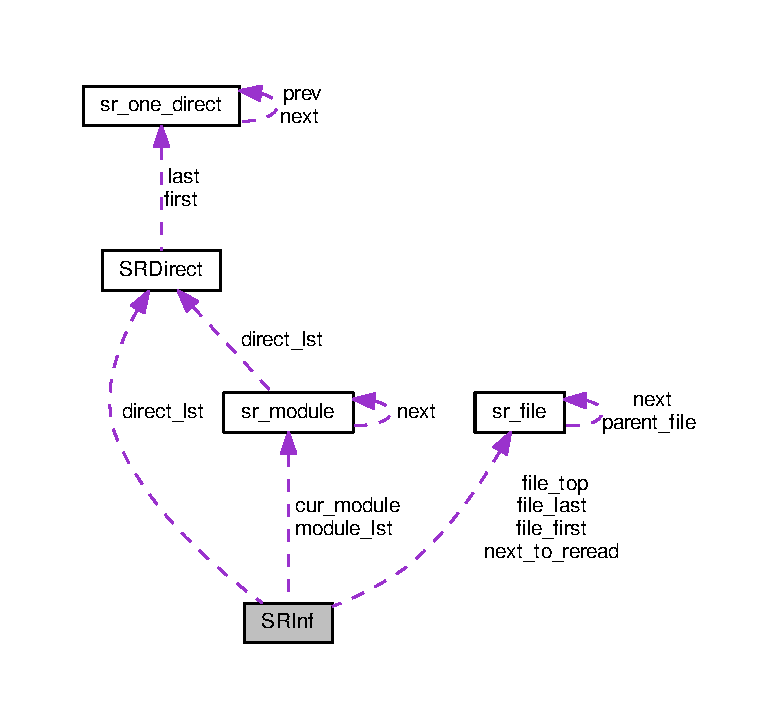
\includegraphics[width=350pt]{structSRInf__coll__graph}
\end{center}
\end{figure}
\subsection*{Data Fields}
\begin{DoxyCompactItemize}
\item 
\hyperlink{bool_8h_afdcfe6db5bea87bd493a3fe2c513d5ef}{Bool} \hyperlink{structSRInf_aa39907250f5d85ed33c6dcb588884cf4}{in\+\_\+use}
\item 
\hyperlink{bool_8h_afdcfe6db5bea87bd493a3fe2c513d5ef}{Bool} \hyperlink{structSRInf_ad7cc53b67596fdc3ac6b6598bfecfff9}{close\+\_\+master\+\_\+at\+\_\+end}
\item 
int \hyperlink{structSRInf_a33cee5de53e9f02597de121734102fa6}{mask}
\item 
\hyperlink{src__rdr__c_8c_a0823532f1e34f34125b37981ad9220ad}{S\+R\+File} $\ast$ \hyperlink{structSRInf_ad34362a8fd8521ebea63e79cd6696ecb}{file\+\_\+first}
\item 
\hyperlink{src__rdr__c_8c_a0823532f1e34f34125b37981ad9220ad}{S\+R\+File} $\ast$ \hyperlink{structSRInf_acb431dfff6fa3e8cbbd8dbfb25c798e8}{file\+\_\+last}
\item 
\hyperlink{src__rdr__c_8c_a0823532f1e34f34125b37981ad9220ad}{S\+R\+File} $\ast$ \hyperlink{structSRInf_a9a0f8d054d9dc2307211b7ef398b8290}{file\+\_\+top}
\item 
\hyperlink{src__rdr__c_8c_a0823532f1e34f34125b37981ad9220ad}{S\+R\+File} $\ast$ \hyperlink{structSRInf_afa0401eba053150cf9e719858d47f22b}{next\+\_\+to\+\_\+reread}
\item 
int \hyperlink{structSRInf_ad3d8ebbeb44105deeb678ceff8b2cb6b}{cur\+\_\+l1}
\item 
int \hyperlink{structSRInf_a9d3a07534c6e60d8b5ffb55a19b17533}{cur\+\_\+l2}
\item 
int \hyperlink{structSRInf_a1ed1a5e79f3f409ca8e28f59830e9ece}{char\+\_\+count}
\item 
int \hyperlink{structSRInf_aa63231d051d7fba34831d0be05e1f8cd}{line\+\_\+count}
\item 
int \hyperlink{structSRInf_af2257adc69f0b5ee25c89a2b33b6c074}{error\+\_\+count}
\item 
int \hyperlink{structSRInf_a432e213e2296877a22dd6e174cb65586}{warning\+\_\+count}
\item 
int \hyperlink{structSRInf_af83f16042ade6e52ac4859f203ef0db4}{out\+\_\+sora\+\_\+word}
\item 
\hyperlink{structSRDirect}{S\+R\+Direct} \hyperlink{structSRInf_a54874ef3dc4c403e8913a9fa4e85158e}{direct\+\_\+lst}
\item 
\hyperlink{src__rdr__c_8c_ad36cf18d86a9a8ac83341b0ea1ce8308}{S\+R\+Module} $\ast$ \hyperlink{structSRInf_a3562e122c09ab0c9eabb4b1d21a86408}{module\+\_\+lst}
\item 
\hyperlink{src__rdr__c_8c_ad36cf18d86a9a8ac83341b0ea1ce8308}{S\+R\+Module} $\ast$ \hyperlink{structSRInf_a791b120048e8a53ac8e6b172c3b33ea2}{cur\+\_\+module}
\item 
\hyperlink{bool_8h_afdcfe6db5bea87bd493a3fe2c513d5ef}{Bool} \hyperlink{structSRInf_af83fb089c4c9359b0d80cbe96bd01adc}{interface}
\end{DoxyCompactItemize}


\subsection{Field Documentation}
\index{S\+R\+Inf@{S\+R\+Inf}!char\+\_\+count@{char\+\_\+count}}
\index{char\+\_\+count@{char\+\_\+count}!S\+R\+Inf@{S\+R\+Inf}}
\subsubsection[{\texorpdfstring{char\+\_\+count}{char_count}}]{\setlength{\rightskip}{0pt plus 5cm}int S\+R\+Inf\+::char\+\_\+count}\hypertarget{structSRInf_a1ed1a5e79f3f409ca8e28f59830e9ece}{}\label{structSRInf_a1ed1a5e79f3f409ca8e28f59830e9ece}
\index{S\+R\+Inf@{S\+R\+Inf}!close\+\_\+master\+\_\+at\+\_\+end@{close\+\_\+master\+\_\+at\+\_\+end}}
\index{close\+\_\+master\+\_\+at\+\_\+end@{close\+\_\+master\+\_\+at\+\_\+end}!S\+R\+Inf@{S\+R\+Inf}}
\subsubsection[{\texorpdfstring{close\+\_\+master\+\_\+at\+\_\+end}{close_master_at_end}}]{\setlength{\rightskip}{0pt plus 5cm}{\bf Bool} S\+R\+Inf\+::close\+\_\+master\+\_\+at\+\_\+end}\hypertarget{structSRInf_ad7cc53b67596fdc3ac6b6598bfecfff9}{}\label{structSRInf_ad7cc53b67596fdc3ac6b6598bfecfff9}
\index{S\+R\+Inf@{S\+R\+Inf}!cur\+\_\+l1@{cur\+\_\+l1}}
\index{cur\+\_\+l1@{cur\+\_\+l1}!S\+R\+Inf@{S\+R\+Inf}}
\subsubsection[{\texorpdfstring{cur\+\_\+l1}{cur_l1}}]{\setlength{\rightskip}{0pt plus 5cm}int S\+R\+Inf\+::cur\+\_\+l1}\hypertarget{structSRInf_ad3d8ebbeb44105deeb678ceff8b2cb6b}{}\label{structSRInf_ad3d8ebbeb44105deeb678ceff8b2cb6b}
\index{S\+R\+Inf@{S\+R\+Inf}!cur\+\_\+l2@{cur\+\_\+l2}}
\index{cur\+\_\+l2@{cur\+\_\+l2}!S\+R\+Inf@{S\+R\+Inf}}
\subsubsection[{\texorpdfstring{cur\+\_\+l2}{cur_l2}}]{\setlength{\rightskip}{0pt plus 5cm}int S\+R\+Inf\+::cur\+\_\+l2}\hypertarget{structSRInf_a9d3a07534c6e60d8b5ffb55a19b17533}{}\label{structSRInf_a9d3a07534c6e60d8b5ffb55a19b17533}
\index{S\+R\+Inf@{S\+R\+Inf}!cur\+\_\+module@{cur\+\_\+module}}
\index{cur\+\_\+module@{cur\+\_\+module}!S\+R\+Inf@{S\+R\+Inf}}
\subsubsection[{\texorpdfstring{cur\+\_\+module}{cur_module}}]{\setlength{\rightskip}{0pt plus 5cm}{\bf S\+R\+Module}$\ast$ S\+R\+Inf\+::cur\+\_\+module}\hypertarget{structSRInf_a791b120048e8a53ac8e6b172c3b33ea2}{}\label{structSRInf_a791b120048e8a53ac8e6b172c3b33ea2}
\index{S\+R\+Inf@{S\+R\+Inf}!direct\+\_\+lst@{direct\+\_\+lst}}
\index{direct\+\_\+lst@{direct\+\_\+lst}!S\+R\+Inf@{S\+R\+Inf}}
\subsubsection[{\texorpdfstring{direct\+\_\+lst}{direct_lst}}]{\setlength{\rightskip}{0pt plus 5cm}{\bf S\+R\+Direct} S\+R\+Inf\+::direct\+\_\+lst}\hypertarget{structSRInf_a54874ef3dc4c403e8913a9fa4e85158e}{}\label{structSRInf_a54874ef3dc4c403e8913a9fa4e85158e}
\index{S\+R\+Inf@{S\+R\+Inf}!error\+\_\+count@{error\+\_\+count}}
\index{error\+\_\+count@{error\+\_\+count}!S\+R\+Inf@{S\+R\+Inf}}
\subsubsection[{\texorpdfstring{error\+\_\+count}{error_count}}]{\setlength{\rightskip}{0pt plus 5cm}int S\+R\+Inf\+::error\+\_\+count}\hypertarget{structSRInf_af2257adc69f0b5ee25c89a2b33b6c074}{}\label{structSRInf_af2257adc69f0b5ee25c89a2b33b6c074}
\index{S\+R\+Inf@{S\+R\+Inf}!file\+\_\+first@{file\+\_\+first}}
\index{file\+\_\+first@{file\+\_\+first}!S\+R\+Inf@{S\+R\+Inf}}
\subsubsection[{\texorpdfstring{file\+\_\+first}{file_first}}]{\setlength{\rightskip}{0pt plus 5cm}{\bf S\+R\+File}$\ast$ S\+R\+Inf\+::file\+\_\+first}\hypertarget{structSRInf_ad34362a8fd8521ebea63e79cd6696ecb}{}\label{structSRInf_ad34362a8fd8521ebea63e79cd6696ecb}
\index{S\+R\+Inf@{S\+R\+Inf}!file\+\_\+last@{file\+\_\+last}}
\index{file\+\_\+last@{file\+\_\+last}!S\+R\+Inf@{S\+R\+Inf}}
\subsubsection[{\texorpdfstring{file\+\_\+last}{file_last}}]{\setlength{\rightskip}{0pt plus 5cm}{\bf S\+R\+File}$\ast$ S\+R\+Inf\+::file\+\_\+last}\hypertarget{structSRInf_acb431dfff6fa3e8cbbd8dbfb25c798e8}{}\label{structSRInf_acb431dfff6fa3e8cbbd8dbfb25c798e8}
\index{S\+R\+Inf@{S\+R\+Inf}!file\+\_\+top@{file\+\_\+top}}
\index{file\+\_\+top@{file\+\_\+top}!S\+R\+Inf@{S\+R\+Inf}}
\subsubsection[{\texorpdfstring{file\+\_\+top}{file_top}}]{\setlength{\rightskip}{0pt plus 5cm}{\bf S\+R\+File}$\ast$ S\+R\+Inf\+::file\+\_\+top}\hypertarget{structSRInf_a9a0f8d054d9dc2307211b7ef398b8290}{}\label{structSRInf_a9a0f8d054d9dc2307211b7ef398b8290}
\index{S\+R\+Inf@{S\+R\+Inf}!in\+\_\+use@{in\+\_\+use}}
\index{in\+\_\+use@{in\+\_\+use}!S\+R\+Inf@{S\+R\+Inf}}
\subsubsection[{\texorpdfstring{in\+\_\+use}{in_use}}]{\setlength{\rightskip}{0pt plus 5cm}{\bf Bool} S\+R\+Inf\+::in\+\_\+use}\hypertarget{structSRInf_aa39907250f5d85ed33c6dcb588884cf4}{}\label{structSRInf_aa39907250f5d85ed33c6dcb588884cf4}
\index{S\+R\+Inf@{S\+R\+Inf}!interface@{interface}}
\index{interface@{interface}!S\+R\+Inf@{S\+R\+Inf}}
\subsubsection[{\texorpdfstring{interface}{interface}}]{\setlength{\rightskip}{0pt plus 5cm}{\bf Bool} S\+R\+Inf\+::interface}\hypertarget{structSRInf_af83fb089c4c9359b0d80cbe96bd01adc}{}\label{structSRInf_af83fb089c4c9359b0d80cbe96bd01adc}
\index{S\+R\+Inf@{S\+R\+Inf}!line\+\_\+count@{line\+\_\+count}}
\index{line\+\_\+count@{line\+\_\+count}!S\+R\+Inf@{S\+R\+Inf}}
\subsubsection[{\texorpdfstring{line\+\_\+count}{line_count}}]{\setlength{\rightskip}{0pt plus 5cm}int S\+R\+Inf\+::line\+\_\+count}\hypertarget{structSRInf_aa63231d051d7fba34831d0be05e1f8cd}{}\label{structSRInf_aa63231d051d7fba34831d0be05e1f8cd}
\index{S\+R\+Inf@{S\+R\+Inf}!mask@{mask}}
\index{mask@{mask}!S\+R\+Inf@{S\+R\+Inf}}
\subsubsection[{\texorpdfstring{mask}{mask}}]{\setlength{\rightskip}{0pt plus 5cm}int S\+R\+Inf\+::mask}\hypertarget{structSRInf_a33cee5de53e9f02597de121734102fa6}{}\label{structSRInf_a33cee5de53e9f02597de121734102fa6}
\index{S\+R\+Inf@{S\+R\+Inf}!module\+\_\+lst@{module\+\_\+lst}}
\index{module\+\_\+lst@{module\+\_\+lst}!S\+R\+Inf@{S\+R\+Inf}}
\subsubsection[{\texorpdfstring{module\+\_\+lst}{module_lst}}]{\setlength{\rightskip}{0pt plus 5cm}{\bf S\+R\+Module}$\ast$ S\+R\+Inf\+::module\+\_\+lst}\hypertarget{structSRInf_a3562e122c09ab0c9eabb4b1d21a86408}{}\label{structSRInf_a3562e122c09ab0c9eabb4b1d21a86408}
\index{S\+R\+Inf@{S\+R\+Inf}!next\+\_\+to\+\_\+reread@{next\+\_\+to\+\_\+reread}}
\index{next\+\_\+to\+\_\+reread@{next\+\_\+to\+\_\+reread}!S\+R\+Inf@{S\+R\+Inf}}
\subsubsection[{\texorpdfstring{next\+\_\+to\+\_\+reread}{next_to_reread}}]{\setlength{\rightskip}{0pt plus 5cm}{\bf S\+R\+File}$\ast$ S\+R\+Inf\+::next\+\_\+to\+\_\+reread}\hypertarget{structSRInf_afa0401eba053150cf9e719858d47f22b}{}\label{structSRInf_afa0401eba053150cf9e719858d47f22b}
\index{S\+R\+Inf@{S\+R\+Inf}!out\+\_\+sora\+\_\+word@{out\+\_\+sora\+\_\+word}}
\index{out\+\_\+sora\+\_\+word@{out\+\_\+sora\+\_\+word}!S\+R\+Inf@{S\+R\+Inf}}
\subsubsection[{\texorpdfstring{out\+\_\+sora\+\_\+word}{out_sora_word}}]{\setlength{\rightskip}{0pt plus 5cm}int S\+R\+Inf\+::out\+\_\+sora\+\_\+word}\hypertarget{structSRInf_af83f16042ade6e52ac4859f203ef0db4}{}\label{structSRInf_af83f16042ade6e52ac4859f203ef0db4}
\index{S\+R\+Inf@{S\+R\+Inf}!warning\+\_\+count@{warning\+\_\+count}}
\index{warning\+\_\+count@{warning\+\_\+count}!S\+R\+Inf@{S\+R\+Inf}}
\subsubsection[{\texorpdfstring{warning\+\_\+count}{warning_count}}]{\setlength{\rightskip}{0pt plus 5cm}int S\+R\+Inf\+::warning\+\_\+count}\hypertarget{structSRInf_a432e213e2296877a22dd6e174cb65586}{}\label{structSRInf_a432e213e2296877a22dd6e174cb65586}


The documentation for this struct was generated from the following file\+:\begin{DoxyCompactItemize}
\item 
gprolog-\/utf8-\/tree/src/\+Bips\+Pl/\hyperlink{src__rdr__c_8c}{src\+\_\+rdr\+\_\+c.\+c}\end{DoxyCompactItemize}

\hypertarget{structStackInf}{}\section{Stack\+Inf Struct Reference}
\label{structStackInf}\index{Stack\+Inf@{Stack\+Inf}}
\subsection*{Data Fields}
\begin{DoxyCompactItemize}
\item 
char {\bfseries name} \mbox{[}32\mbox{]}\hypertarget{structStackInf_a9f47cfd7dc989579d8e449ac821130ce}{}\label{structStackInf_a9f47cfd7dc989579d8e449ac821130ce}

\item 
char {\bfseries desc} \mbox{[}64\mbox{]}\hypertarget{structStackInf_a6719b7ffffaa34f3a5c973e06369e9b3}{}\label{structStackInf_a6719b7ffffaa34f3a5c973e06369e9b3}

\item 
int {\bfseries def\+\_\+size}\hypertarget{structStackInf_a58879eae3bfda4bb51d864f58ba32b8f}{}\label{structStackInf_a58879eae3bfda4bb51d864f58ba32b8f}

\item 
char {\bfseries top\+\_\+macro} \mbox{[}128\mbox{]}\hypertarget{structStackInf_aecd772924d9909d2875259c5aedc5bc9}{}\label{structStackInf_aecd772924d9909d2875259c5aedc5bc9}

\end{DoxyCompactItemize}


The documentation for this struct was generated from the following file\+:\begin{DoxyCompactItemize}
\item 
gprolog-\/utf8-\/tree/src/\+Engine\+Pl/pl\+\_\+config.\+c\end{DoxyCompactItemize}

\hypertarget{structstm__inf}{}\section{stm\+\_\+inf Struct Reference}
\label{structstm__inf}\index{stm\+\_\+inf@{stm\+\_\+inf}}


Collaboration diagram for stm\+\_\+inf\+:\nopagebreak
\begin{figure}[H]
\begin{center}
\leavevmode
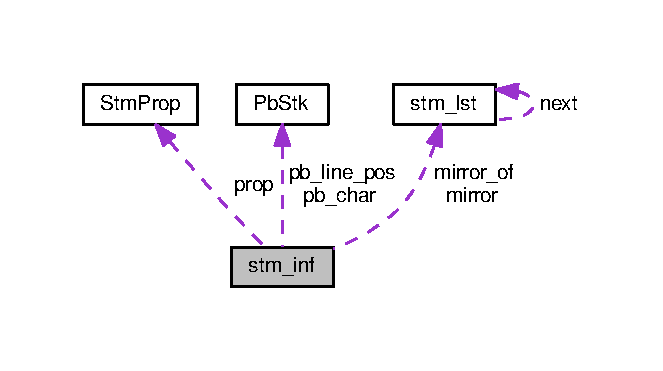
\includegraphics[width=318pt]{structstm__inf__coll__graph}
\end{center}
\end{figure}
\subsection*{Data Fields}
\begin{DoxyCompactItemize}
\item 
int {\bfseries atom\+\_\+file\+\_\+name}\hypertarget{structstm__inf_a9dc8280c20f516cfce88bdacfc1c70e9}{}\label{structstm__inf_a9dc8280c20f516cfce88bdacfc1c70e9}

\item 
Pl\+Long {\bfseries file}\hypertarget{structstm__inf_a85bc801ede0cd63b9a7a9cacb839bc98}{}\label{structstm__inf_a85bc801ede0cd63b9a7a9cacb839bc98}

\item 
\hyperlink{structStmProp}{Stm\+Prop} {\bfseries prop}\hypertarget{structstm__inf_a5b984f4df0d32f07741b75dced7453aa}{}\label{structstm__inf_a5b984f4df0d32f07741b75dced7453aa}

\item 
\hyperlink{structstm__lst}{Stm\+Lst} $\ast$ {\bfseries mirror}\hypertarget{structstm__inf_a2e13c8b109418f635fabba678006c6cd}{}\label{structstm__inf_a2e13c8b109418f635fabba678006c6cd}

\item 
\hyperlink{structstm__lst}{Stm\+Lst} $\ast$ {\bfseries mirror\+\_\+of}\hypertarget{structstm__inf_ada3cbffaa477959332fc96000cc4b73e}{}\label{structstm__inf_ada3cbffaa477959332fc96000cc4b73e}

\item 
Stm\+Fct {\bfseries fct\+\_\+getc}\hypertarget{structstm__inf_a1ff7dd59a7e0a7b8eaf540cc5ad8145e}{}\label{structstm__inf_a1ff7dd59a7e0a7b8eaf540cc5ad8145e}

\item 
Stm\+Fct {\bfseries fct\+\_\+putc}\hypertarget{structstm__inf_aeba256b0be0d697ad8563fd3475e26d2}{}\label{structstm__inf_aeba256b0be0d697ad8563fd3475e26d2}

\item 
Stm\+Fct {\bfseries fct\+\_\+flush}\hypertarget{structstm__inf_a32fe5f685abc6990b6da6020eb004b60}{}\label{structstm__inf_a32fe5f685abc6990b6da6020eb004b60}

\item 
Stm\+Fct {\bfseries fct\+\_\+close}\hypertarget{structstm__inf_a5f6fd03e09577d0f7ba5c600d35d3ad8}{}\label{structstm__inf_a5f6fd03e09577d0f7ba5c600d35d3ad8}

\item 
Stm\+Fct {\bfseries fct\+\_\+tell}\hypertarget{structstm__inf_a1f829218b8f5b09925cb45caec5af199}{}\label{structstm__inf_a1f829218b8f5b09925cb45caec5af199}

\item 
Stm\+Fct {\bfseries fct\+\_\+seek}\hypertarget{structstm__inf_a5f9d4068bafcdf0a8ced688439af8aa2}{}\label{structstm__inf_a5f9d4068bafcdf0a8ced688439af8aa2}

\item 
Stm\+Fct {\bfseries fct\+\_\+clearerr}\hypertarget{structstm__inf_afaf9188c97510a5f1d612e1444f6e801}{}\label{structstm__inf_afaf9188c97510a5f1d612e1444f6e801}

\item 
Bool {\bfseries eof\+\_\+reached}\hypertarget{structstm__inf_ac3960253b7e5f826635a196b096fd499}{}\label{structstm__inf_ac3960253b7e5f826635a196b096fd499}

\item 
\hyperlink{structPbStk}{Pb\+Stk} {\bfseries pb\+\_\+char}\hypertarget{structstm__inf_af66229bdb1421dc62daaee808af84bba}{}\label{structstm__inf_af66229bdb1421dc62daaee808af84bba}

\item 
Pl\+Long {\bfseries char\+\_\+count}\hypertarget{structstm__inf_a0c6895ef7d7a03c6f0ad2aa05be2c0af}{}\label{structstm__inf_a0c6895ef7d7a03c6f0ad2aa05be2c0af}

\item 
Pl\+Long {\bfseries line\+\_\+count}\hypertarget{structstm__inf_a0394c04b8f2bd5990d30dd6ad14a8246}{}\label{structstm__inf_a0394c04b8f2bd5990d30dd6ad14a8246}

\item 
Pl\+Long {\bfseries line\+\_\+pos}\hypertarget{structstm__inf_a89769bf2d0ca17434b431c380379e674}{}\label{structstm__inf_a89769bf2d0ca17434b431c380379e674}

\item 
\hyperlink{structPbStk}{Pb\+Stk} {\bfseries pb\+\_\+line\+\_\+pos}\hypertarget{structstm__inf_acd4b4b0e220c45642fb4a6903d6ec4d5}{}\label{structstm__inf_acd4b4b0e220c45642fb4a6903d6ec4d5}

\end{DoxyCompactItemize}


The documentation for this struct was generated from the following file\+:\begin{DoxyCompactItemize}
\item 
gprolog-\/utf8-\/tree/src/\+Bips\+Pl/stream\+\_\+supp.\+h\end{DoxyCompactItemize}

\hypertarget{structstm__lst}{}\section{stm\+\_\+lst Struct Reference}
\label{structstm__lst}\index{stm\+\_\+lst@{stm\+\_\+lst}}


{\ttfamily \#include $<$stream\+\_\+supp.\+h$>$}



Collaboration diagram for stm\+\_\+lst\+:\nopagebreak
\begin{figure}[H]
\begin{center}
\leavevmode
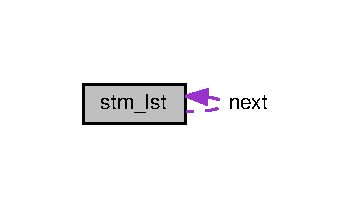
\includegraphics[width=169pt]{structstm__lst__coll__graph}
\end{center}
\end{figure}
\subsection*{Data Fields}
\begin{DoxyCompactItemize}
\item 
int \hyperlink{structstm__lst_a69932b67f84be652c1d4fab80820a4cc}{stm}
\item 
\hyperlink{stream__supp_8h_a6b553ae1ecc32ad49304cd836fb357c3}{P\+Stm\+Lst} \hyperlink{structstm__lst_aaecf8566184bb06365a7de2d3ba8312b}{next}
\end{DoxyCompactItemize}


\subsection{Field Documentation}
\index{stm\+\_\+lst@{stm\+\_\+lst}!next@{next}}
\index{next@{next}!stm\+\_\+lst@{stm\+\_\+lst}}
\subsubsection[{\texorpdfstring{next}{next}}]{\setlength{\rightskip}{0pt plus 5cm}{\bf P\+Stm\+Lst} stm\+\_\+lst\+::next}\hypertarget{structstm__lst_aaecf8566184bb06365a7de2d3ba8312b}{}\label{structstm__lst_aaecf8566184bb06365a7de2d3ba8312b}
\index{stm\+\_\+lst@{stm\+\_\+lst}!stm@{stm}}
\index{stm@{stm}!stm\+\_\+lst@{stm\+\_\+lst}}
\subsubsection[{\texorpdfstring{stm}{stm}}]{\setlength{\rightskip}{0pt plus 5cm}int stm\+\_\+lst\+::stm}\hypertarget{structstm__lst_a69932b67f84be652c1d4fab80820a4cc}{}\label{structstm__lst_a69932b67f84be652c1d4fab80820a4cc}


The documentation for this struct was generated from the following file\+:\begin{DoxyCompactItemize}
\item 
gprolog-\/utf8-\/tree/src/\+Bips\+Pl/\hyperlink{stream__supp_8h}{stream\+\_\+supp.\+h}\end{DoxyCompactItemize}

\hypertarget{structStmProp}{}\section{Stm\+Prop Struct Reference}
\label{structStmProp}\index{Stm\+Prop@{Stm\+Prop}}
\subsection*{Data Fields}
\begin{DoxyCompactItemize}
\item 
unsigned {\bfseries mode}\+:2\hypertarget{structStmProp_a8a2ef413513d1963d66e2f490b6b83b4}{}\label{structStmProp_a8a2ef413513d1963d66e2f490b6b83b4}

\item 
unsigned {\bfseries input}\+:1\hypertarget{structStmProp_a600c8a2fc85ea28e18dd45a1bfdbb039}{}\label{structStmProp_a600c8a2fc85ea28e18dd45a1bfdbb039}

\item 
unsigned {\bfseries output}\+:1\hypertarget{structStmProp_ac00a5a24dbbfeece3814be64cc7014d6}{}\label{structStmProp_ac00a5a24dbbfeece3814be64cc7014d6}

\item 
unsigned {\bfseries text}\+:1\hypertarget{structStmProp_ac19d8844240a9c3059104f8afd135834}{}\label{structStmProp_ac19d8844240a9c3059104f8afd135834}

\item 
unsigned {\bfseries reposition}\+:1\hypertarget{structStmProp_a812b9e484fea9756ace87645f847f6f4}{}\label{structStmProp_a812b9e484fea9756ace87645f847f6f4}

\item 
unsigned {\bfseries eof\+\_\+action}\+:2\hypertarget{structStmProp_a04e464b0b01bd6e61e4752dc40264126}{}\label{structStmProp_a04e464b0b01bd6e61e4752dc40264126}

\item 
unsigned {\bfseries buffering}\+:2\hypertarget{structStmProp_ad4122d8a077810116d89eb216c24e642}{}\label{structStmProp_ad4122d8a077810116d89eb216c24e642}

\item 
unsigned {\bfseries special\+\_\+close}\+:1\hypertarget{structStmProp_a77078202569393e5ac5b40c0e3b4e8af}{}\label{structStmProp_a77078202569393e5ac5b40c0e3b4e8af}

\item 
unsigned {\bfseries other}\+:8\hypertarget{structStmProp_a53b858c5848ca920087838eb02faf75f}{}\label{structStmProp_a53b858c5848ca920087838eb02faf75f}

\end{DoxyCompactItemize}


The documentation for this struct was generated from the following file\+:\begin{DoxyCompactItemize}
\item 
gprolog-\/utf8-\/tree/src/\+Bips\+Pl/stream\+\_\+supp.\+h\end{DoxyCompactItemize}

\hypertarget{structStrSInf}{}\section{Str\+S\+Inf Struct Reference}
\label{structStrSInf}\index{Str\+S\+Inf@{Str\+S\+Inf}}


{\ttfamily \#include $<$stream\+\_\+supp.\+h$>$}

\subsection*{Data Fields}
\begin{DoxyCompactItemize}
\item 
char $\ast$ \hyperlink{structStrSInf_aeb057f9f00adf6340a825b3a5f5d2f85}{buff}
\item 
char $\ast$ \hyperlink{structStrSInf_a68da0c71b6666b73881d68d364de63f2}{ptr}
\item 
\hyperlink{bool_8h_afdcfe6db5bea87bd493a3fe2c513d5ef}{Bool} \hyperlink{structStrSInf_af4eb3705492f95c32af035b64b070958}{buff\+\_\+alloc\+\_\+size}
\end{DoxyCompactItemize}


\subsection{Field Documentation}
\index{Str\+S\+Inf@{Str\+S\+Inf}!buff@{buff}}
\index{buff@{buff}!Str\+S\+Inf@{Str\+S\+Inf}}
\subsubsection[{\texorpdfstring{buff}{buff}}]{\setlength{\rightskip}{0pt plus 5cm}char$\ast$ Str\+S\+Inf\+::buff}\hypertarget{structStrSInf_aeb057f9f00adf6340a825b3a5f5d2f85}{}\label{structStrSInf_aeb057f9f00adf6340a825b3a5f5d2f85}
\index{Str\+S\+Inf@{Str\+S\+Inf}!buff\+\_\+alloc\+\_\+size@{buff\+\_\+alloc\+\_\+size}}
\index{buff\+\_\+alloc\+\_\+size@{buff\+\_\+alloc\+\_\+size}!Str\+S\+Inf@{Str\+S\+Inf}}
\subsubsection[{\texorpdfstring{buff\+\_\+alloc\+\_\+size}{buff_alloc_size}}]{\setlength{\rightskip}{0pt plus 5cm}{\bf Bool} Str\+S\+Inf\+::buff\+\_\+alloc\+\_\+size}\hypertarget{structStrSInf_af4eb3705492f95c32af035b64b070958}{}\label{structStrSInf_af4eb3705492f95c32af035b64b070958}
\index{Str\+S\+Inf@{Str\+S\+Inf}!ptr@{ptr}}
\index{ptr@{ptr}!Str\+S\+Inf@{Str\+S\+Inf}}
\subsubsection[{\texorpdfstring{ptr}{ptr}}]{\setlength{\rightskip}{0pt plus 5cm}char$\ast$ Str\+S\+Inf\+::ptr}\hypertarget{structStrSInf_a68da0c71b6666b73881d68d364de63f2}{}\label{structStrSInf_a68da0c71b6666b73881d68d364de63f2}


The documentation for this struct was generated from the following file\+:\begin{DoxyCompactItemize}
\item 
gprolog-\/utf8-\/tree/src/\+Bips\+Pl/\hyperlink{stream__supp_8h}{stream\+\_\+supp.\+h}\end{DoxyCompactItemize}

\hypertarget{structswt__elt}{}\section{swt\+\_\+elt Struct Reference}
\label{structswt__elt}\index{swt\+\_\+elt@{swt\+\_\+elt}}


Collaboration diagram for swt\+\_\+elt\+:\nopagebreak
\begin{figure}[H]
\begin{center}
\leavevmode
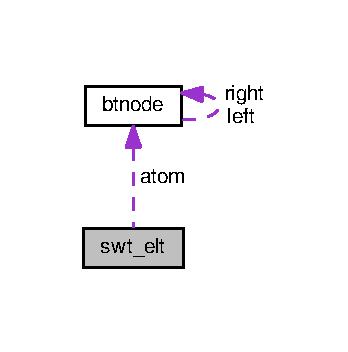
\includegraphics[width=167pt]{structswt__elt__coll__graph}
\end{center}
\end{figure}
\subsection*{Data Fields}
\begin{DoxyCompactItemize}
\item 
\hyperlink{bt__string_8h_a94e2311ccccb66fae2c4ce55649526fc}{B\+T\+Node} $\ast$ \hyperlink{structswt__elt_a04d09a38ab072084ef44f3b17a75b25d}{atom}
\item 
\hyperlink{gprolog_8h_a4d005b136d7fb28537eb1815f7868b63}{Pl\+Long} \hyperlink{structswt__elt_aa3fb3cf68a09b57a7abad92d1888d297}{n}
\item 
\hyperlink{gprolog_8h_a4d005b136d7fb28537eb1815f7868b63}{Pl\+Long} \hyperlink{structswt__elt_a979d2691c64643e5d59f471a3e5e40f6}{label}
\end{DoxyCompactItemize}


\subsection{Field Documentation}
\index{swt\+\_\+elt@{swt\+\_\+elt}!atom@{atom}}
\index{atom@{atom}!swt\+\_\+elt@{swt\+\_\+elt}}
\subsubsection[{\texorpdfstring{atom}{atom}}]{\setlength{\rightskip}{0pt plus 5cm}{\bf B\+T\+Node}$\ast$ swt\+\_\+elt\+::atom}\hypertarget{structswt__elt_a04d09a38ab072084ef44f3b17a75b25d}{}\label{structswt__elt_a04d09a38ab072084ef44f3b17a75b25d}
\index{swt\+\_\+elt@{swt\+\_\+elt}!label@{label}}
\index{label@{label}!swt\+\_\+elt@{swt\+\_\+elt}}
\subsubsection[{\texorpdfstring{label}{label}}]{\setlength{\rightskip}{0pt plus 5cm}{\bf Pl\+Long} swt\+\_\+elt\+::label}\hypertarget{structswt__elt_a979d2691c64643e5d59f471a3e5e40f6}{}\label{structswt__elt_a979d2691c64643e5d59f471a3e5e40f6}
\index{swt\+\_\+elt@{swt\+\_\+elt}!n@{n}}
\index{n@{n}!swt\+\_\+elt@{swt\+\_\+elt}}
\subsubsection[{\texorpdfstring{n}{n}}]{\setlength{\rightskip}{0pt plus 5cm}{\bf Pl\+Long} swt\+\_\+elt\+::n}\hypertarget{structswt__elt_aa3fb3cf68a09b57a7abad92d1888d297}{}\label{structswt__elt_aa3fb3cf68a09b57a7abad92d1888d297}


The documentation for this struct was generated from the following file\+:\begin{DoxyCompactItemize}
\item 
gprolog-\/utf8-\/tree/src/\+Wam2\+Ma/\hyperlink{wam2ma_8c}{wam2ma.\+c}\end{DoxyCompactItemize}

\hypertarget{structswt__tbl}{}\section{swt\+\_\+tbl Struct Reference}
\label{structswt__tbl}\index{swt\+\_\+tbl@{swt\+\_\+tbl}}


Collaboration diagram for swt\+\_\+tbl\+:\nopagebreak
\begin{figure}[H]
\begin{center}
\leavevmode
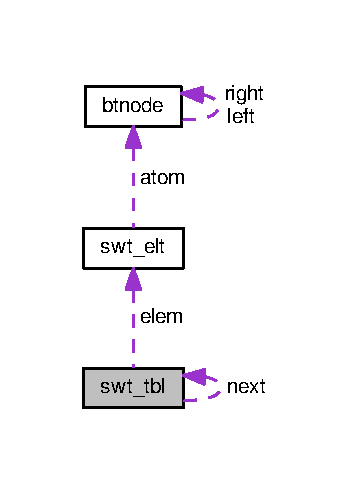
\includegraphics[width=168pt]{structswt__tbl__coll__graph}
\end{center}
\end{figure}
\subsection*{Public Types}
\begin{DoxyCompactItemize}
\item 
enum \{ {\bfseries T\+B\+L\+\_\+\+A\+TM}, 
{\bfseries T\+B\+L\+\_\+\+I\+NT}, 
{\bfseries T\+B\+L\+\_\+\+S\+TC}
 \}\hypertarget{structswt__tbl_a6e6eca39872e41e6d834af855ee073b9}{}\label{structswt__tbl_a6e6eca39872e41e6d834af855ee073b9}

\end{DoxyCompactItemize}
\subsection*{Data Fields}
\begin{DoxyCompactItemize}
\item 
enum swt\+\_\+tbl\+:: \{ ... \}  {\bfseries type}\hypertarget{structswt__tbl_a6b1e4dc1e07f951ebe6ea23a9567e0ca}{}\label{structswt__tbl_a6b1e4dc1e07f951ebe6ea23a9567e0ca}

\item 
int {\bfseries tbl\+\_\+no}\hypertarget{structswt__tbl_a83f05356288e3c0f11cf0539a4a64eaa}{}\label{structswt__tbl_a83f05356288e3c0f11cf0539a4a64eaa}

\item 
\hyperlink{structswt__tbl}{P\+Swt\+Tbl} {\bfseries next}\hypertarget{structswt__tbl_aed3e3921525480876c83cfab6c82ae3b}{}\label{structswt__tbl_aed3e3921525480876c83cfab6c82ae3b}

\item 
int {\bfseries nb\+\_\+elem}\hypertarget{structswt__tbl_a1f108cb255f34e0e43fd548bdeaa2a3e}{}\label{structswt__tbl_a1f108cb255f34e0e43fd548bdeaa2a3e}

\item 
\hyperlink{structswt__elt}{Swt\+Elt} {\bfseries elem} \mbox{[}A\+N\+Y\+\_\+\+S\+I\+ZE\mbox{]}\hypertarget{structswt__tbl_aef5072704a328212e05d40837fe665d0}{}\label{structswt__tbl_aef5072704a328212e05d40837fe665d0}

\end{DoxyCompactItemize}


The documentation for this struct was generated from the following file\+:\begin{DoxyCompactItemize}
\item 
gprolog-\/utf8-\/tree/src/\+Wam2\+Ma/wam2ma.\+c\end{DoxyCompactItemize}

\hypertarget{structSwtInf}{}\section{Swt\+Inf Struct Reference}
\label{structSwtInf}\index{Swt\+Inf@{Swt\+Inf}}


{\ttfamily \#include $<$wam\+\_\+inst.\+h$>$}

\subsection*{Data Fields}
\begin{DoxyCompactItemize}
\item 
\hyperlink{gprolog_8h_a4d005b136d7fb28537eb1815f7868b63}{Pl\+Long} \hyperlink{structSwtInf_ad115955219677407a1cf8cdadc8ab19f}{key}
\item 
Code\+Ptr \hyperlink{structSwtInf_a6d3bad3eb0abb1b73b7776d5153c34fd}{codep}
\item 
\hyperlink{gprolog_8h_a4d005b136d7fb28537eb1815f7868b63}{Pl\+Long} \hyperlink{structSwtInf_a31e087797a5ae675b9c0a80344891bbc}{int\+\_\+val}
\item 
char $\ast$ \hyperlink{structSwtInf_aca3187b48d4bc13a963b097f9e228266}{label}
\end{DoxyCompactItemize}


\subsection{Field Documentation}
\index{Swt\+Inf@{Swt\+Inf}!codep@{codep}}
\index{codep@{codep}!Swt\+Inf@{Swt\+Inf}}
\subsubsection[{\texorpdfstring{codep}{codep}}]{\setlength{\rightskip}{0pt plus 5cm}Code\+Ptr Swt\+Inf\+::codep}\hypertarget{structSwtInf_a6d3bad3eb0abb1b73b7776d5153c34fd}{}\label{structSwtInf_a6d3bad3eb0abb1b73b7776d5153c34fd}
\index{Swt\+Inf@{Swt\+Inf}!int\+\_\+val@{int\+\_\+val}}
\index{int\+\_\+val@{int\+\_\+val}!Swt\+Inf@{Swt\+Inf}}
\subsubsection[{\texorpdfstring{int\+\_\+val}{int_val}}]{\setlength{\rightskip}{0pt plus 5cm}{\bf Pl\+Long} Swt\+Inf\+::int\+\_\+val}\hypertarget{structSwtInf_a31e087797a5ae675b9c0a80344891bbc}{}\label{structSwtInf_a31e087797a5ae675b9c0a80344891bbc}
\index{Swt\+Inf@{Swt\+Inf}!key@{key}}
\index{key@{key}!Swt\+Inf@{Swt\+Inf}}
\subsubsection[{\texorpdfstring{key}{key}}]{\setlength{\rightskip}{0pt plus 5cm}{\bf Pl\+Long} Swt\+Inf\+::key}\hypertarget{structSwtInf_ad115955219677407a1cf8cdadc8ab19f}{}\label{structSwtInf_ad115955219677407a1cf8cdadc8ab19f}
\index{Swt\+Inf@{Swt\+Inf}!label@{label}}
\index{label@{label}!Swt\+Inf@{Swt\+Inf}}
\subsubsection[{\texorpdfstring{label}{label}}]{\setlength{\rightskip}{0pt plus 5cm}char$\ast$ Swt\+Inf\+::label}\hypertarget{structSwtInf_aca3187b48d4bc13a963b097f9e228266}{}\label{structSwtInf_aca3187b48d4bc13a963b097f9e228266}


The documentation for this struct was generated from the following files\+:\begin{DoxyCompactItemize}
\item 
gprolog-\/utf8-\/tree/src/\+Engine\+Pl/\hyperlink{wam__inst_8h}{wam\+\_\+inst.\+h}\item 
gprolog-\/utf8-\/tree/src/\+Ma2\+Asm/\hyperlink{ma__parser_8h}{ma\+\_\+parser.\+h}\end{DoxyCompactItemize}

\hypertarget{structTagInf}{}\section{Tag\+Inf Struct Reference}
\label{structTagInf}\index{Tag\+Inf@{Tag\+Inf}}
\subsection*{Data Fields}
\begin{DoxyCompactItemize}
\item 
char {\bfseries name} \mbox{[}32\mbox{]}\hypertarget{structTagInf_a6dc0e60ac19532e7c8e1c30f73357c1c}{}\label{structTagInf_a6dc0e60ac19532e7c8e1c30f73357c1c}

\item 
Typ\+Tag {\bfseries type}\hypertarget{structTagInf_a1d109a0184537c9f448e28aa6c492b91}{}\label{structTagInf_a1d109a0184537c9f448e28aa6c492b91}

\item 
int {\bfseries value}\hypertarget{structTagInf_ae5a47ca79c53423fd961942af0647109}{}\label{structTagInf_ae5a47ca79c53423fd961942af0647109}

\end{DoxyCompactItemize}


The documentation for this struct was generated from the following file\+:\begin{DoxyCompactItemize}
\item 
gprolog-\/utf8-\/tree/src/\+Engine\+Pl/pl\+\_\+config.\+c\end{DoxyCompactItemize}

\hypertarget{structTermSInf}{}\section{Term\+S\+Inf Struct Reference}
\label{structTermSInf}\index{Term\+S\+Inf@{Term\+S\+Inf}}
\subsection*{Data Fields}
\begin{DoxyCompactItemize}
\item 
int {\bfseries buff\+\_\+size}\hypertarget{structTermSInf_aa2ac007b499e0cb03e17072299872d08}{}\label{structTermSInf_aa2ac007b499e0cb03e17072299872d08}

\item 
Bool {\bfseries buff\+\_\+is\+\_\+alloc}\hypertarget{structTermSInf_a02d37582809df8e6a18bf4cdcb598693}{}\label{structTermSInf_a02d37582809df8e6a18bf4cdcb598693}

\item 
char $\ast$ {\bfseries buff}\hypertarget{structTermSInf_aea3421d8fe398941f9280da64bcfba35}{}\label{structTermSInf_aea3421d8fe398941f9280da64bcfba35}

\item 
char $\ast$ {\bfseries ptr}\hypertarget{structTermSInf_a46ab1bf8caba7bd0044429601be6b670}{}\label{structTermSInf_a46ab1bf8caba7bd0044429601be6b670}

\end{DoxyCompactItemize}


The documentation for this struct was generated from the following file\+:\begin{DoxyCompactItemize}
\item 
gprolog-\/utf8-\/tree/src/\+Bips\+Pl/stream\+\_\+c.\+c\end{DoxyCompactItemize}

\hypertarget{structTokInf}{}\section{Tok\+Inf Struct Reference}
\label{structTokInf}\index{Tok\+Inf@{Tok\+Inf}}


{\ttfamily \#include $<$scan\+\_\+supp.\+h$>$}

\subsection*{Data Fields}
\begin{DoxyCompactItemize}
\item 
\hyperlink{scan__supp_8h_a92e3dba2da3b5e64ff0567a8aa779891}{Typ\+Tok} \hyperlink{structTokInf_a9ae46e898f23f677836fa19cc119276b}{type}
\item 
char \hyperlink{structTokInf_aa56c61670fa2e571afc6647c76af2103}{name} \mbox{[}\hyperlink{scan__supp_8h_ac61c2e9163da6fb2b5fcd9a86c88af5d}{S\+C\+A\+N\+\_\+\+B\+I\+G\+\_\+\+B\+U\+F\+F\+ER}\mbox{]}
\item 
int \hyperlink{structTokInf_aedaf8feef7d9708e8a946df56d7cdb66}{quoted}
\item 
int \hyperlink{structTokInf_addc6977c79a52835a28c0347c453df5d}{punct}
\item 
\hyperlink{gprolog_8h_a4d005b136d7fb28537eb1815f7868b63}{Pl\+Long} \hyperlink{structTokInf_a9f5266be5fc6a8e446ed3e660032d0ad}{int\+\_\+num}
\item 
double \hyperlink{structTokInf_afddf6ad76bb496c8ddd35a5b773f4360}{float\+\_\+num}
\item 
int \hyperlink{structTokInf_a141b87290988df7a09d0f84593cd02c5}{line}
\item 
int \hyperlink{structTokInf_a3034cb3570c3c0a946e3e1c86b0464a7}{col}
\end{DoxyCompactItemize}


\subsection{Field Documentation}
\index{Tok\+Inf@{Tok\+Inf}!col@{col}}
\index{col@{col}!Tok\+Inf@{Tok\+Inf}}
\subsubsection[{\texorpdfstring{col}{col}}]{\setlength{\rightskip}{0pt plus 5cm}int Tok\+Inf\+::col}\hypertarget{structTokInf_a3034cb3570c3c0a946e3e1c86b0464a7}{}\label{structTokInf_a3034cb3570c3c0a946e3e1c86b0464a7}
\index{Tok\+Inf@{Tok\+Inf}!float\+\_\+num@{float\+\_\+num}}
\index{float\+\_\+num@{float\+\_\+num}!Tok\+Inf@{Tok\+Inf}}
\subsubsection[{\texorpdfstring{float\+\_\+num}{float_num}}]{\setlength{\rightskip}{0pt plus 5cm}double Tok\+Inf\+::float\+\_\+num}\hypertarget{structTokInf_afddf6ad76bb496c8ddd35a5b773f4360}{}\label{structTokInf_afddf6ad76bb496c8ddd35a5b773f4360}
\index{Tok\+Inf@{Tok\+Inf}!int\+\_\+num@{int\+\_\+num}}
\index{int\+\_\+num@{int\+\_\+num}!Tok\+Inf@{Tok\+Inf}}
\subsubsection[{\texorpdfstring{int\+\_\+num}{int_num}}]{\setlength{\rightskip}{0pt plus 5cm}{\bf Pl\+Long} Tok\+Inf\+::int\+\_\+num}\hypertarget{structTokInf_a9f5266be5fc6a8e446ed3e660032d0ad}{}\label{structTokInf_a9f5266be5fc6a8e446ed3e660032d0ad}
\index{Tok\+Inf@{Tok\+Inf}!line@{line}}
\index{line@{line}!Tok\+Inf@{Tok\+Inf}}
\subsubsection[{\texorpdfstring{line}{line}}]{\setlength{\rightskip}{0pt plus 5cm}int Tok\+Inf\+::line}\hypertarget{structTokInf_a141b87290988df7a09d0f84593cd02c5}{}\label{structTokInf_a141b87290988df7a09d0f84593cd02c5}
\index{Tok\+Inf@{Tok\+Inf}!name@{name}}
\index{name@{name}!Tok\+Inf@{Tok\+Inf}}
\subsubsection[{\texorpdfstring{name}{name}}]{\setlength{\rightskip}{0pt plus 5cm}char Tok\+Inf\+::name\mbox{[}{\bf S\+C\+A\+N\+\_\+\+B\+I\+G\+\_\+\+B\+U\+F\+F\+ER}\mbox{]}}\hypertarget{structTokInf_aa56c61670fa2e571afc6647c76af2103}{}\label{structTokInf_aa56c61670fa2e571afc6647c76af2103}
\index{Tok\+Inf@{Tok\+Inf}!punct@{punct}}
\index{punct@{punct}!Tok\+Inf@{Tok\+Inf}}
\subsubsection[{\texorpdfstring{punct}{punct}}]{\setlength{\rightskip}{0pt plus 5cm}int Tok\+Inf\+::punct}\hypertarget{structTokInf_addc6977c79a52835a28c0347c453df5d}{}\label{structTokInf_addc6977c79a52835a28c0347c453df5d}
\index{Tok\+Inf@{Tok\+Inf}!quoted@{quoted}}
\index{quoted@{quoted}!Tok\+Inf@{Tok\+Inf}}
\subsubsection[{\texorpdfstring{quoted}{quoted}}]{\setlength{\rightskip}{0pt plus 5cm}int Tok\+Inf\+::quoted}\hypertarget{structTokInf_aedaf8feef7d9708e8a946df56d7cdb66}{}\label{structTokInf_aedaf8feef7d9708e8a946df56d7cdb66}
\index{Tok\+Inf@{Tok\+Inf}!type@{type}}
\index{type@{type}!Tok\+Inf@{Tok\+Inf}}
\subsubsection[{\texorpdfstring{type}{type}}]{\setlength{\rightskip}{0pt plus 5cm}{\bf Typ\+Tok} Tok\+Inf\+::type}\hypertarget{structTokInf_a9ae46e898f23f677836fa19cc119276b}{}\label{structTokInf_a9ae46e898f23f677836fa19cc119276b}


The documentation for this struct was generated from the following file\+:\begin{DoxyCompactItemize}
\item 
gprolog-\/utf8-\/tree/src/\+Bips\+Pl/\hyperlink{scan__supp_8h}{scan\+\_\+supp.\+h}\end{DoxyCompactItemize}

\hypertarget{structUsedFile}{}\section{Used\+File Struct Reference}
\label{structUsedFile}\index{Used\+File@{Used\+File}}
\subsection*{Data Fields}
\begin{DoxyCompactItemize}
\item 
char $\ast$ {\bfseries name}\hypertarget{structUsedFile_a8d4ed04924e68784f37a3f3f268ff633}{}\label{structUsedFile_a8d4ed04924e68784f37a3f3f268ff633}

\item 
char $\ast$ {\bfseries parent}\hypertarget{structUsedFile_a3bf412b1901e0513545a138bfdb9b254}{}\label{structUsedFile_a3bf412b1901e0513545a138bfdb9b254}

\item 
int {\bfseries line}\hypertarget{structUsedFile_a5a91641c98e7812d3af04c519499dd5c}{}\label{structUsedFile_a5a91641c98e7812d3af04c519499dd5c}

\end{DoxyCompactItemize}


The documentation for this struct was generated from the following file\+:\begin{DoxyCompactItemize}
\item 
gprolog-\/utf8-\/tree/src/\+Engine\+Pl/cpp\+\_\+headers.\+c\end{DoxyCompactItemize}

\hypertarget{structUsedMachRegInf}{}\section{Used\+Mach\+Reg\+Inf Struct Reference}
\label{structUsedMachRegInf}\index{Used\+Mach\+Reg\+Inf@{Used\+Mach\+Reg\+Inf}}
\subsection*{Data Fields}
\begin{DoxyCompactItemize}
\item 
char $\ast$ {\bfseries mach\+\_\+reg\+\_\+name}\hypertarget{structUsedMachRegInf_a469dabfeaa37fca00d87667d4dacc064}{}\label{structUsedMachRegInf_a469dabfeaa37fca00d87667d4dacc064}

\item 
char $\ast$ {\bfseries pl\+\_\+reg\+\_\+name}\hypertarget{structUsedMachRegInf_a9a0e95f20d942e8610a0e905bafc7353}{}\label{structUsedMachRegInf_a9a0e95f20d942e8610a0e905bafc7353}

\item 
char $\ast$ {\bfseries type}\hypertarget{structUsedMachRegInf_a2e0c08014802409c0a340c61fab7dafe}{}\label{structUsedMachRegInf_a2e0c08014802409c0a340c61fab7dafe}

\end{DoxyCompactItemize}


The documentation for this struct was generated from the following file\+:\begin{DoxyCompactItemize}
\item 
gprolog-\/utf8-\/tree/src/\+Engine\+Pl/pl\+\_\+config.\+c\end{DoxyCompactItemize}

%--- End generated contents ---

% Index
\backmatter
\newpage
\phantomsection
\clearemptydoublepage
\addcontentsline{toc}{chapter}{Index}
\printindex

\end{document}
